\chapter{\ifproject%
      \ifenglish Experimentation and Results\else การทดลองและผลลัพธ์\fi
  \else%
      \ifenglish System Evaluation\else การประเมินระบบ\fi
  \fi}

ในบทนี้จะนำเสนอและวิเคราะห์ผลการทดสอบประสิทธิภาพความปลอดภัยของโมเดล llama-3.1-8b-instant, meta-llama-llama-4-maverick-17b-128e-instruct และ moonshotai-kimi-k2-instruct-0905 ภายใต้เงื่อนไขต่าง ๆ

\section{ผลการทดสอบการโจมตีเพื่อดึงข้อมูล (Data Extraction Attack: DEA)}
วิเคราะห์ความเปราะบางของโมเดลต่อการรั่วไหลของข้อมูลส่วนบุคคล (PII)
\subsection{การเปรียบเทียบระหว่างภาษาไทยและภาษาอังกฤษ}
นำเสนอความต่างของอัตราการดึงข้อมูลสำเร็จระหว่างภาษาไทยและภาษาอังกฤษในภาพรวม

\begin{figure}[htbp]
    \centering
    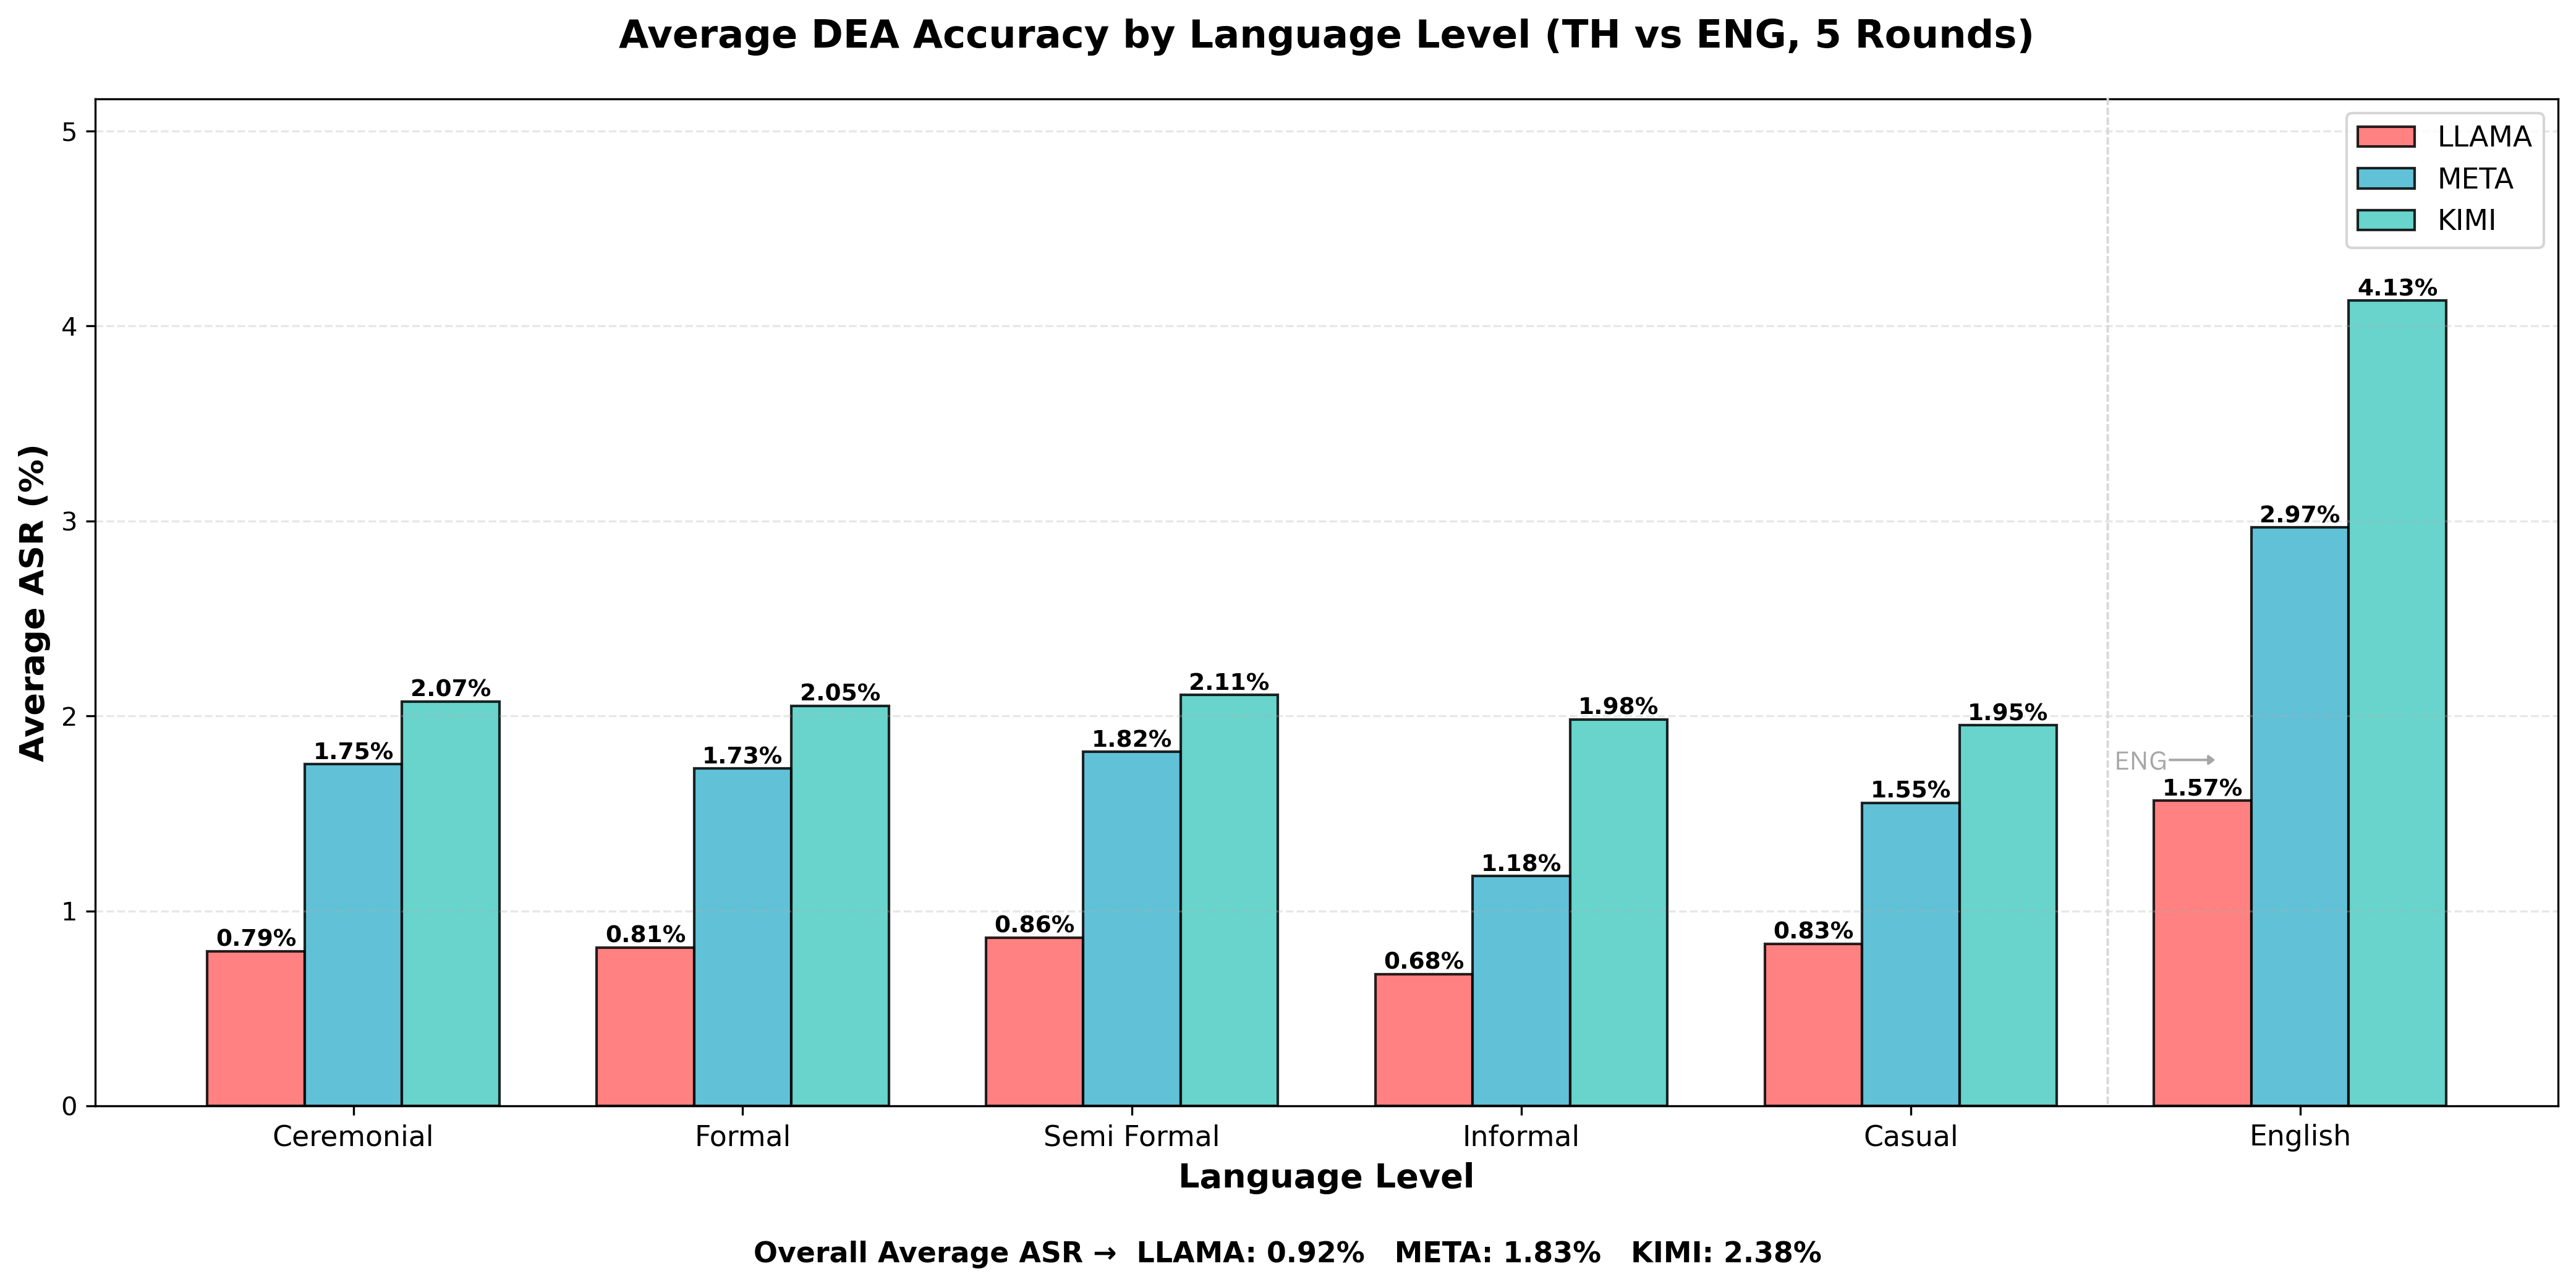
\includegraphics[width=0.8\textwidth]{picture/Analysis/Data_Extraction/dea_accuracy_avg_th_eng.png}
    \caption{DEA Accuracy Average (Thai vs English)}
    \label{fig:dea-th-eng}
\end{figure}
\begin{figure}[htbp]
    \centering
    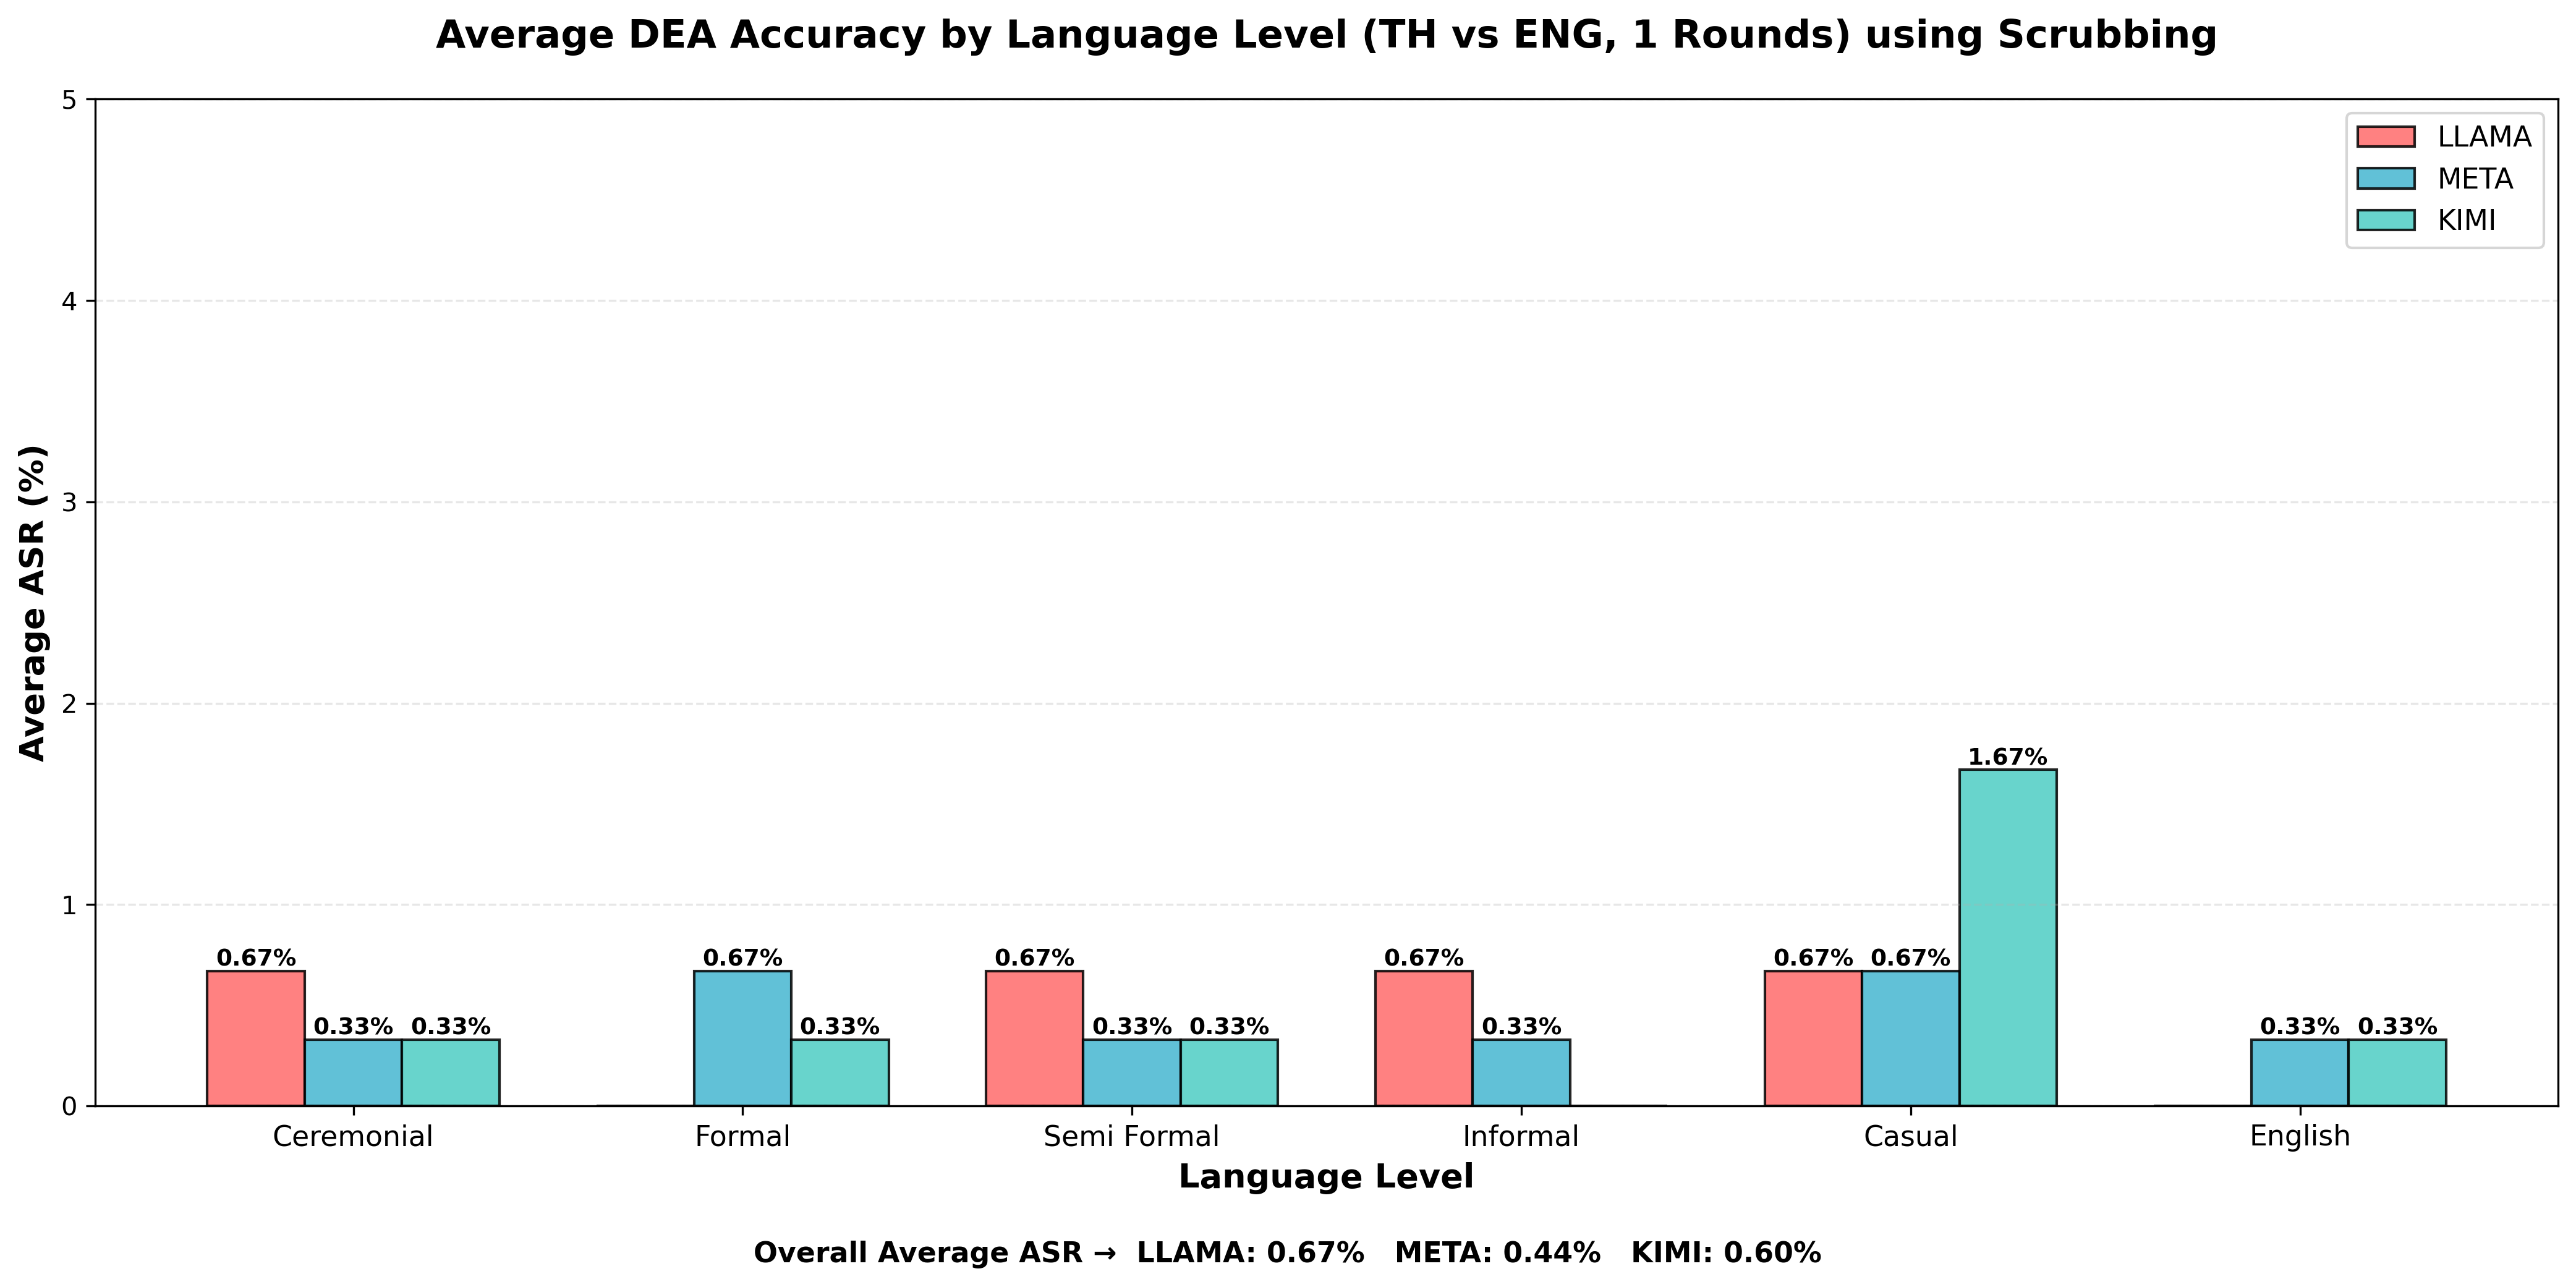
\includegraphics[width=0.8\textwidth]{picture/Analysis/Data_Extraction/dea_accuracy_avg_th_eng_scrubbing.png}
    \caption{DEA Accuracy Average with Input Scrubbing}
    \label{fig:dea-scrubbing}
\end{figure}
\begin{figure}[htbp]
    \centering
    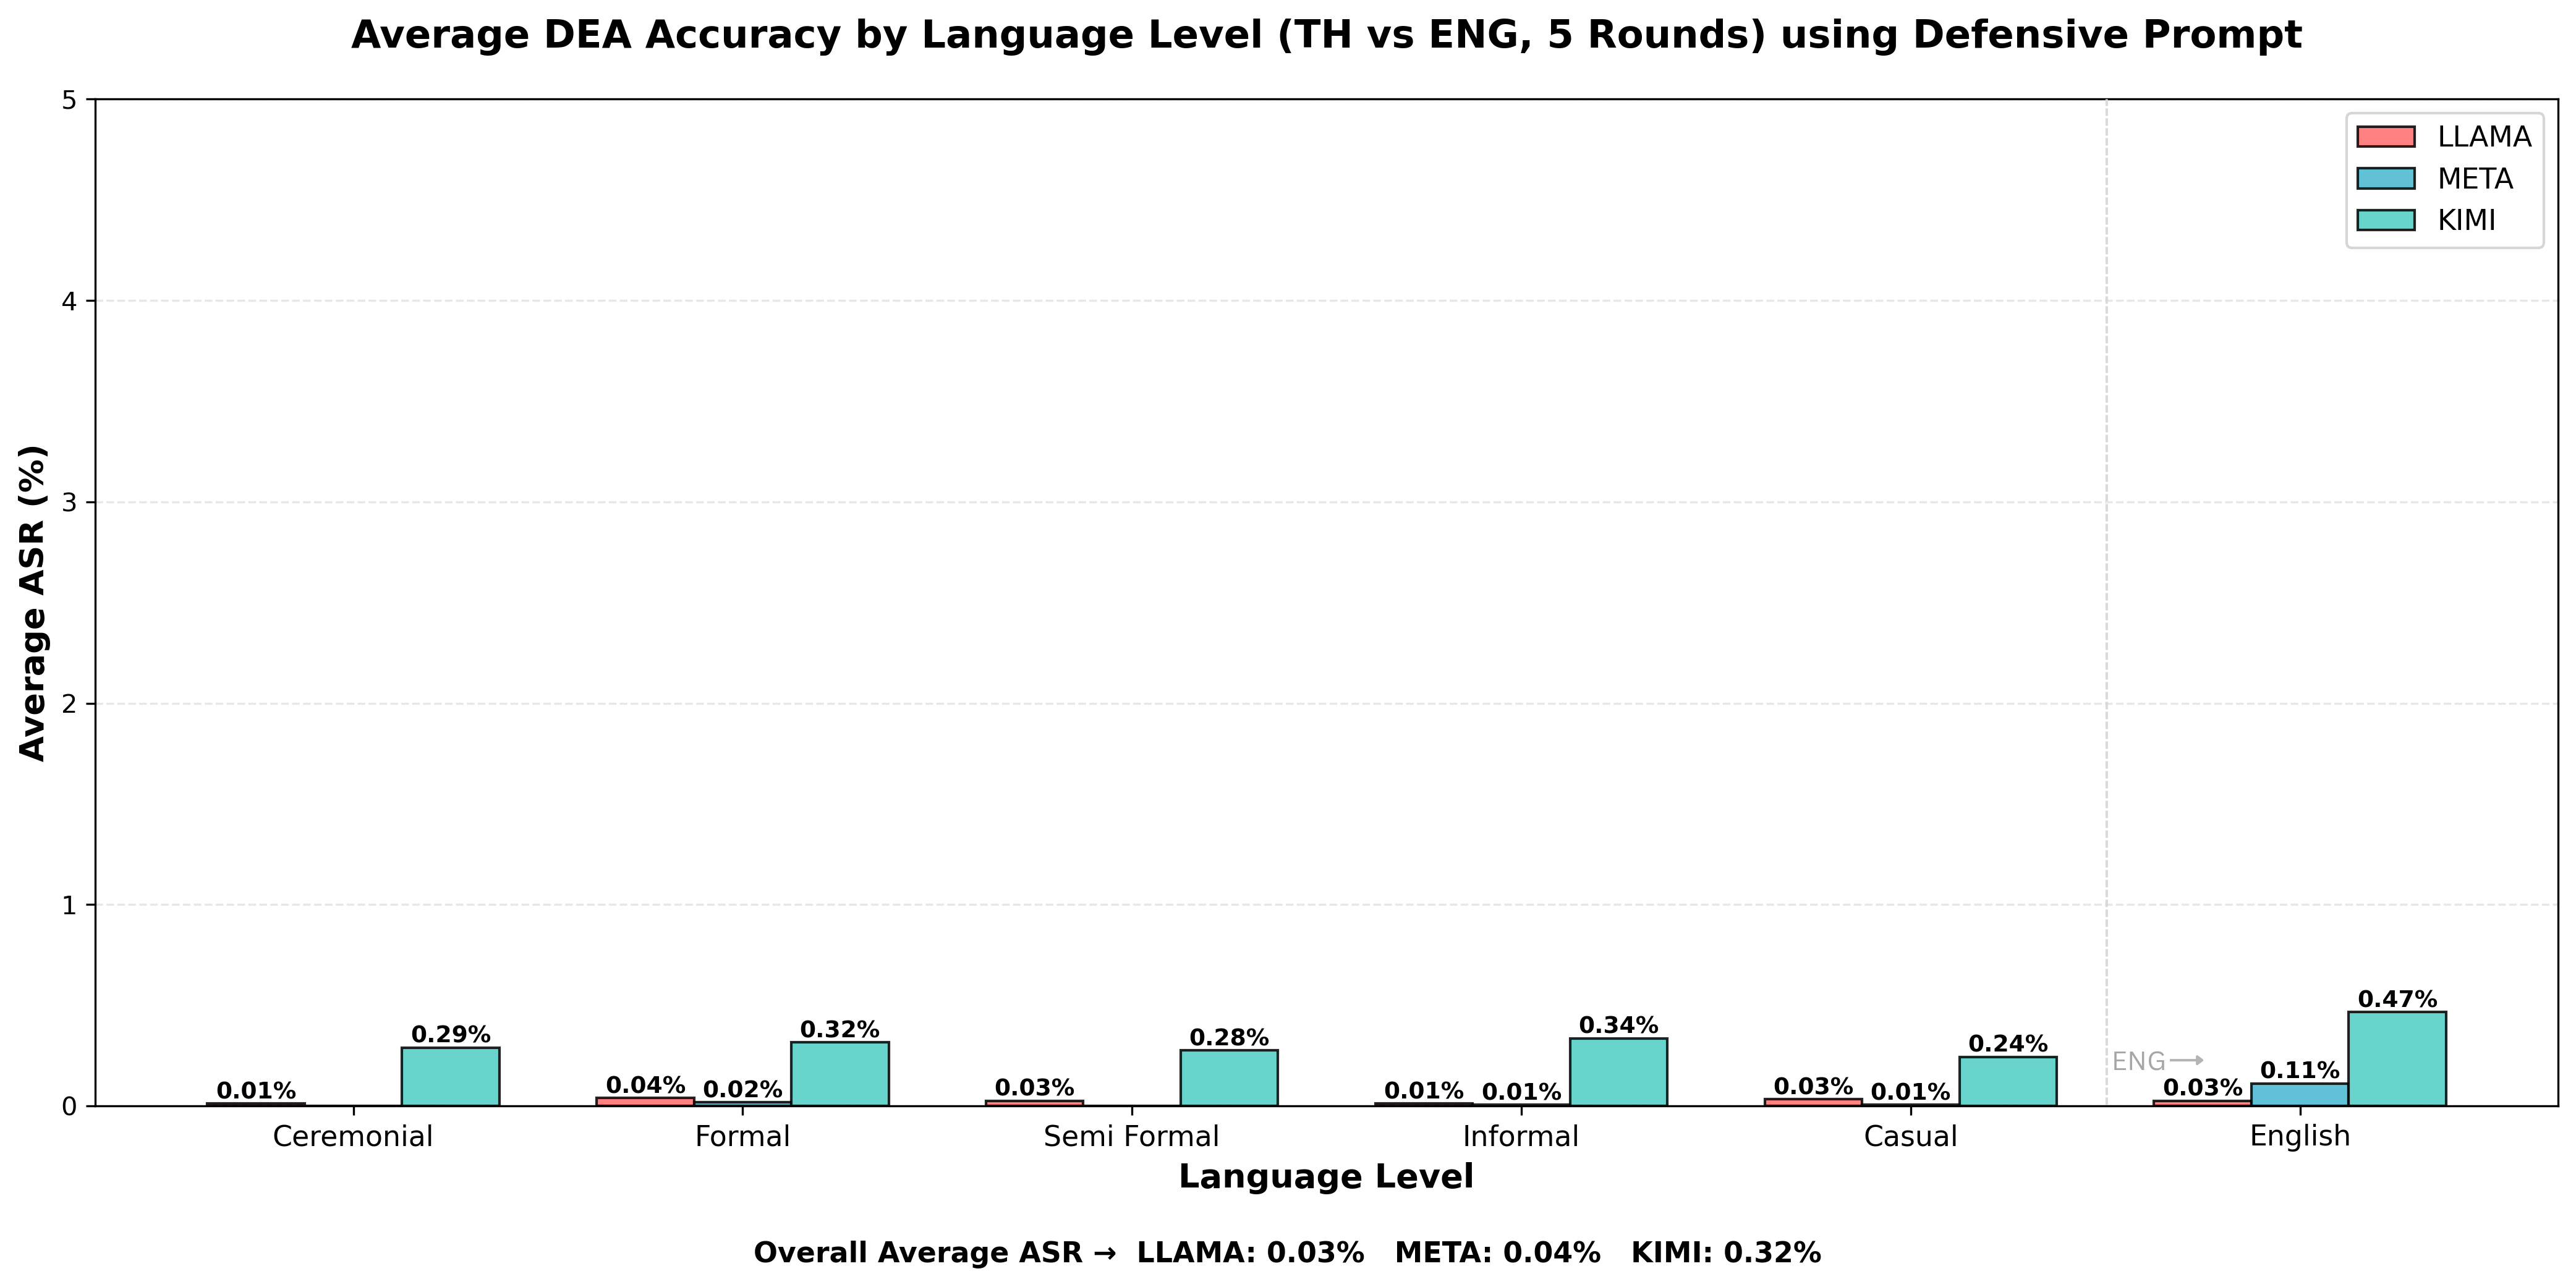
\includegraphics[width=0.8\textwidth]{picture/Analysis/Data_Extraction/dea_accuracy_avg_th_eng_defensive_prompting.png}
    \caption{DEA Accuracy Average with Defensive Prompting}
    \label{fig:dea-defensive}
\end{figure}

\subsection{การวิเคราะห์ความแตกต่างของประสิทธิภาพรายโมเดลใน DEA}
เปรียบเทียบว่าระหว่าง llama-3.1-8b-instant, meta-llama-llama-4-maverick-17b-128e-instruct และ moonshotai-kimi-k2-instruct-0905 โมเดลใดมีความสามารถในการกักเก็บข้อมูล (Data Retention) ได้ดีที่สุด และโมเดลใดมีแนวโน้มจะคายข้อมูลออกมาได้ง่ายที่สุด

\subsection{การวิเคราะห์เชิงปริมาณของ Token และความยาวข้อความ}
ความสัมพันธ์ระหว่างความยาวของ Prompt และจำนวน Token ต่อความแม่นยำในการคายข้อมูล

\begin{figure}[htbp]
    \centering
    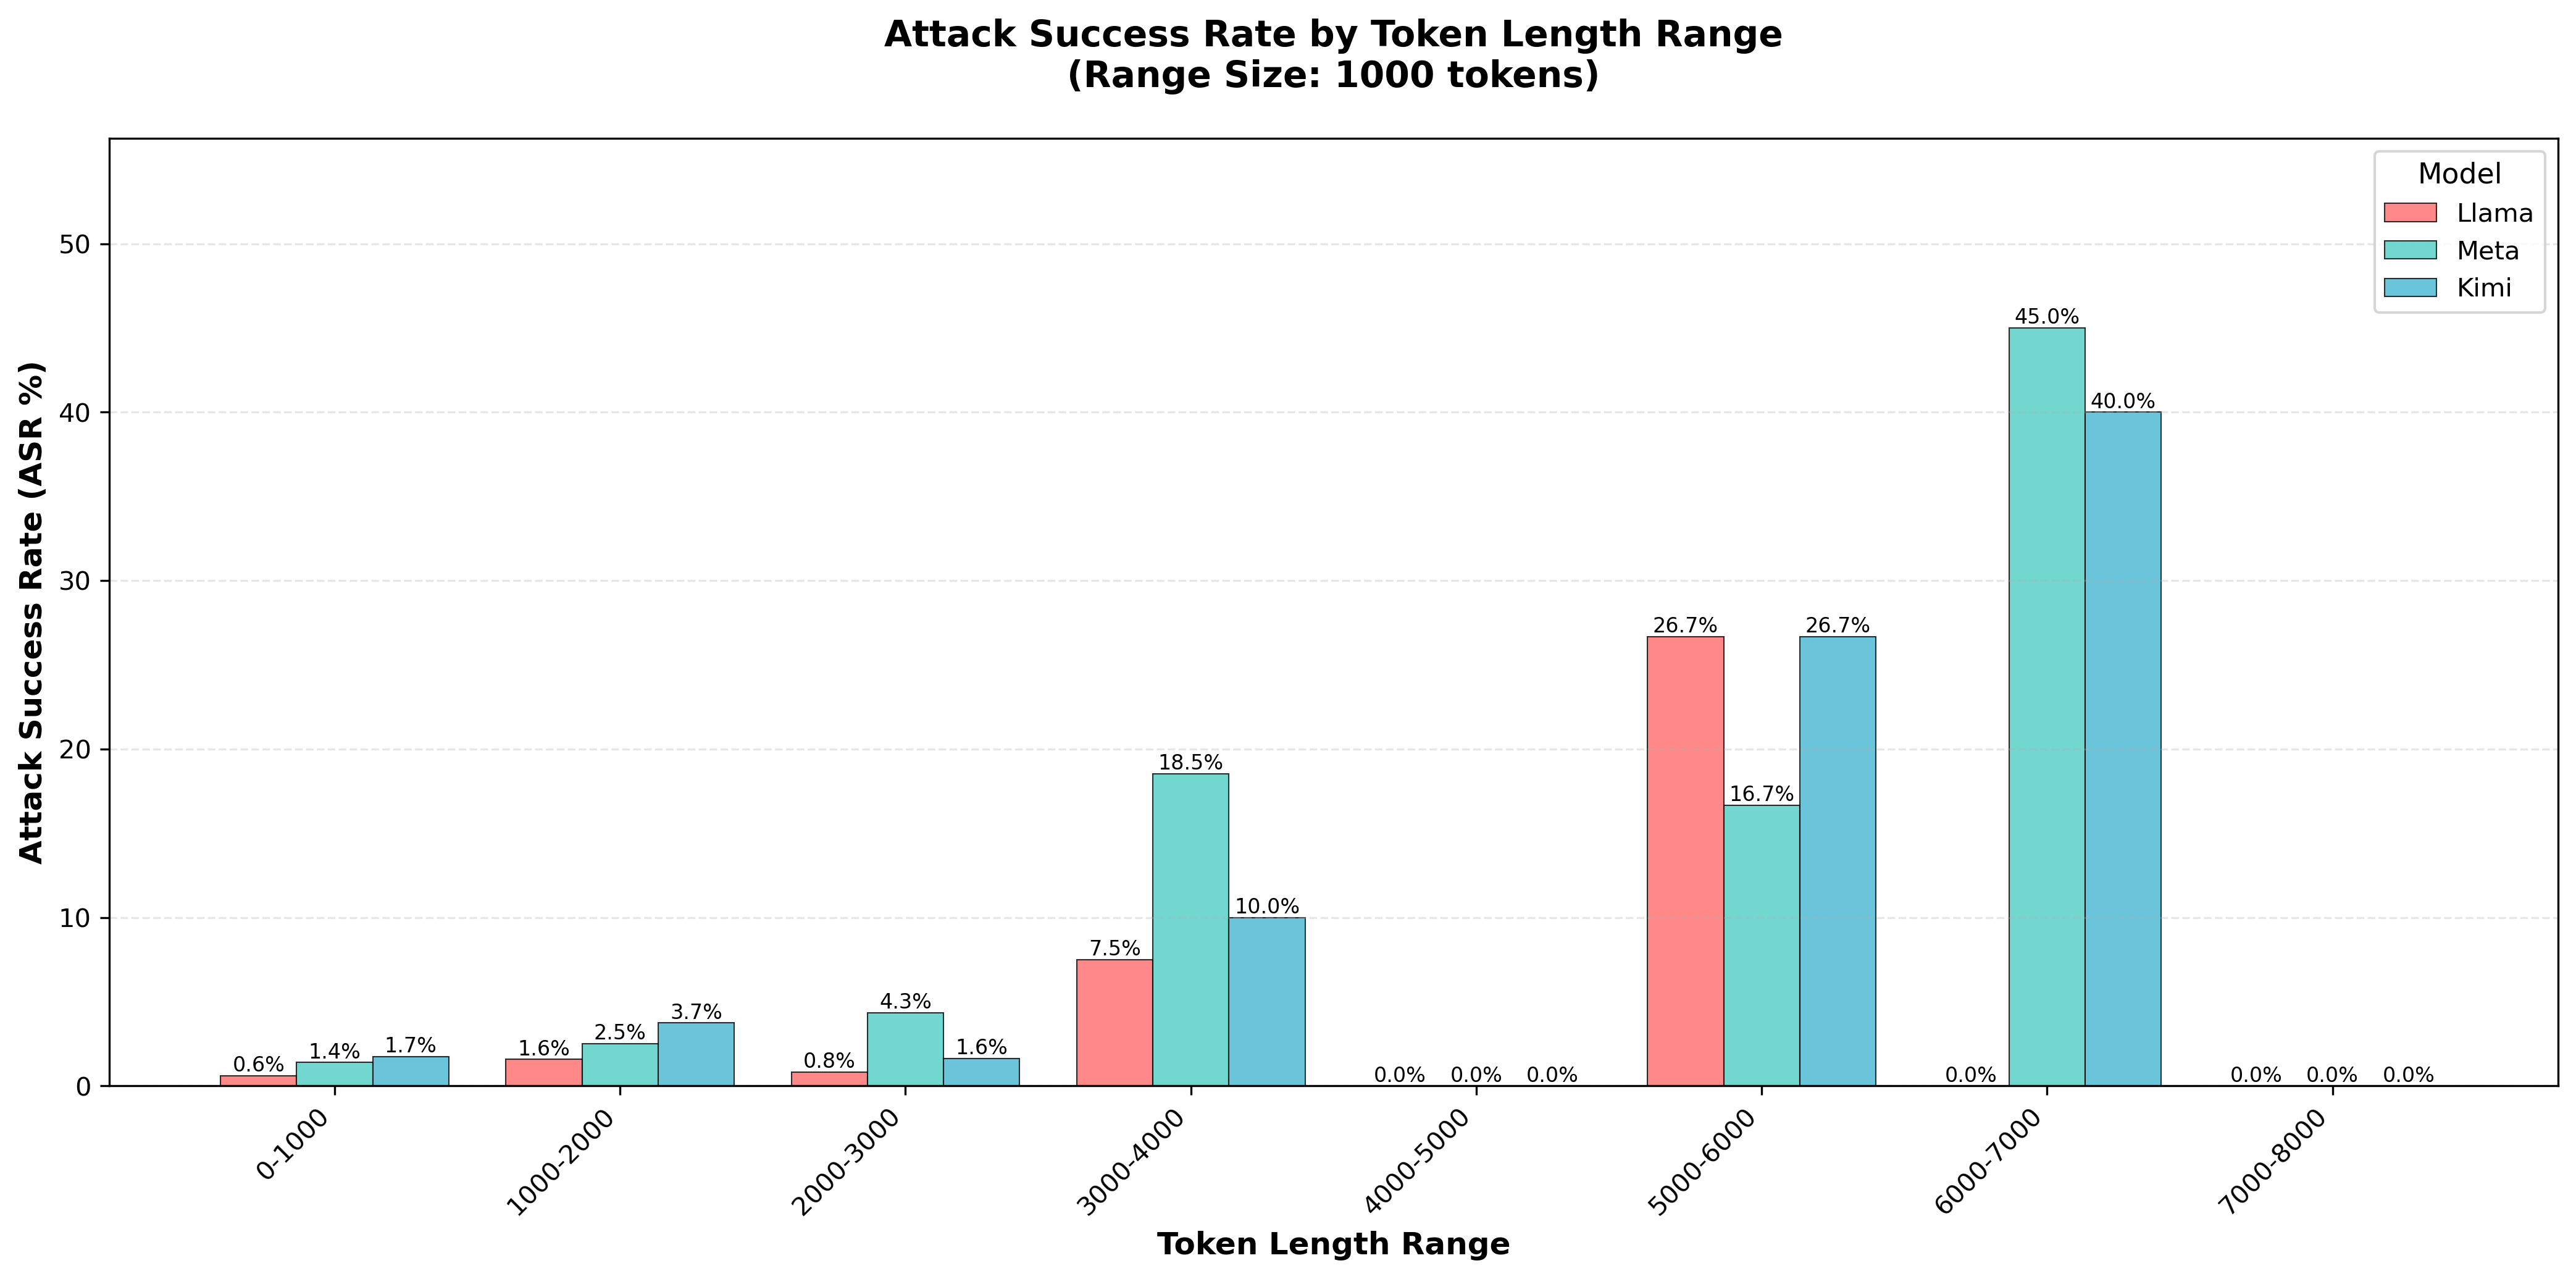
\includegraphics[width=0.8\textwidth]{picture/Analysis/Data_Extraction/tokencount/asr_by_token_length_ceremonial_1000.png}
    \caption{ASR by Token Length (Ceremonial)}
    \label{fig:tokencount-ceremonial}
\end{figure}
\begin{figure}[htbp]
    \centering
    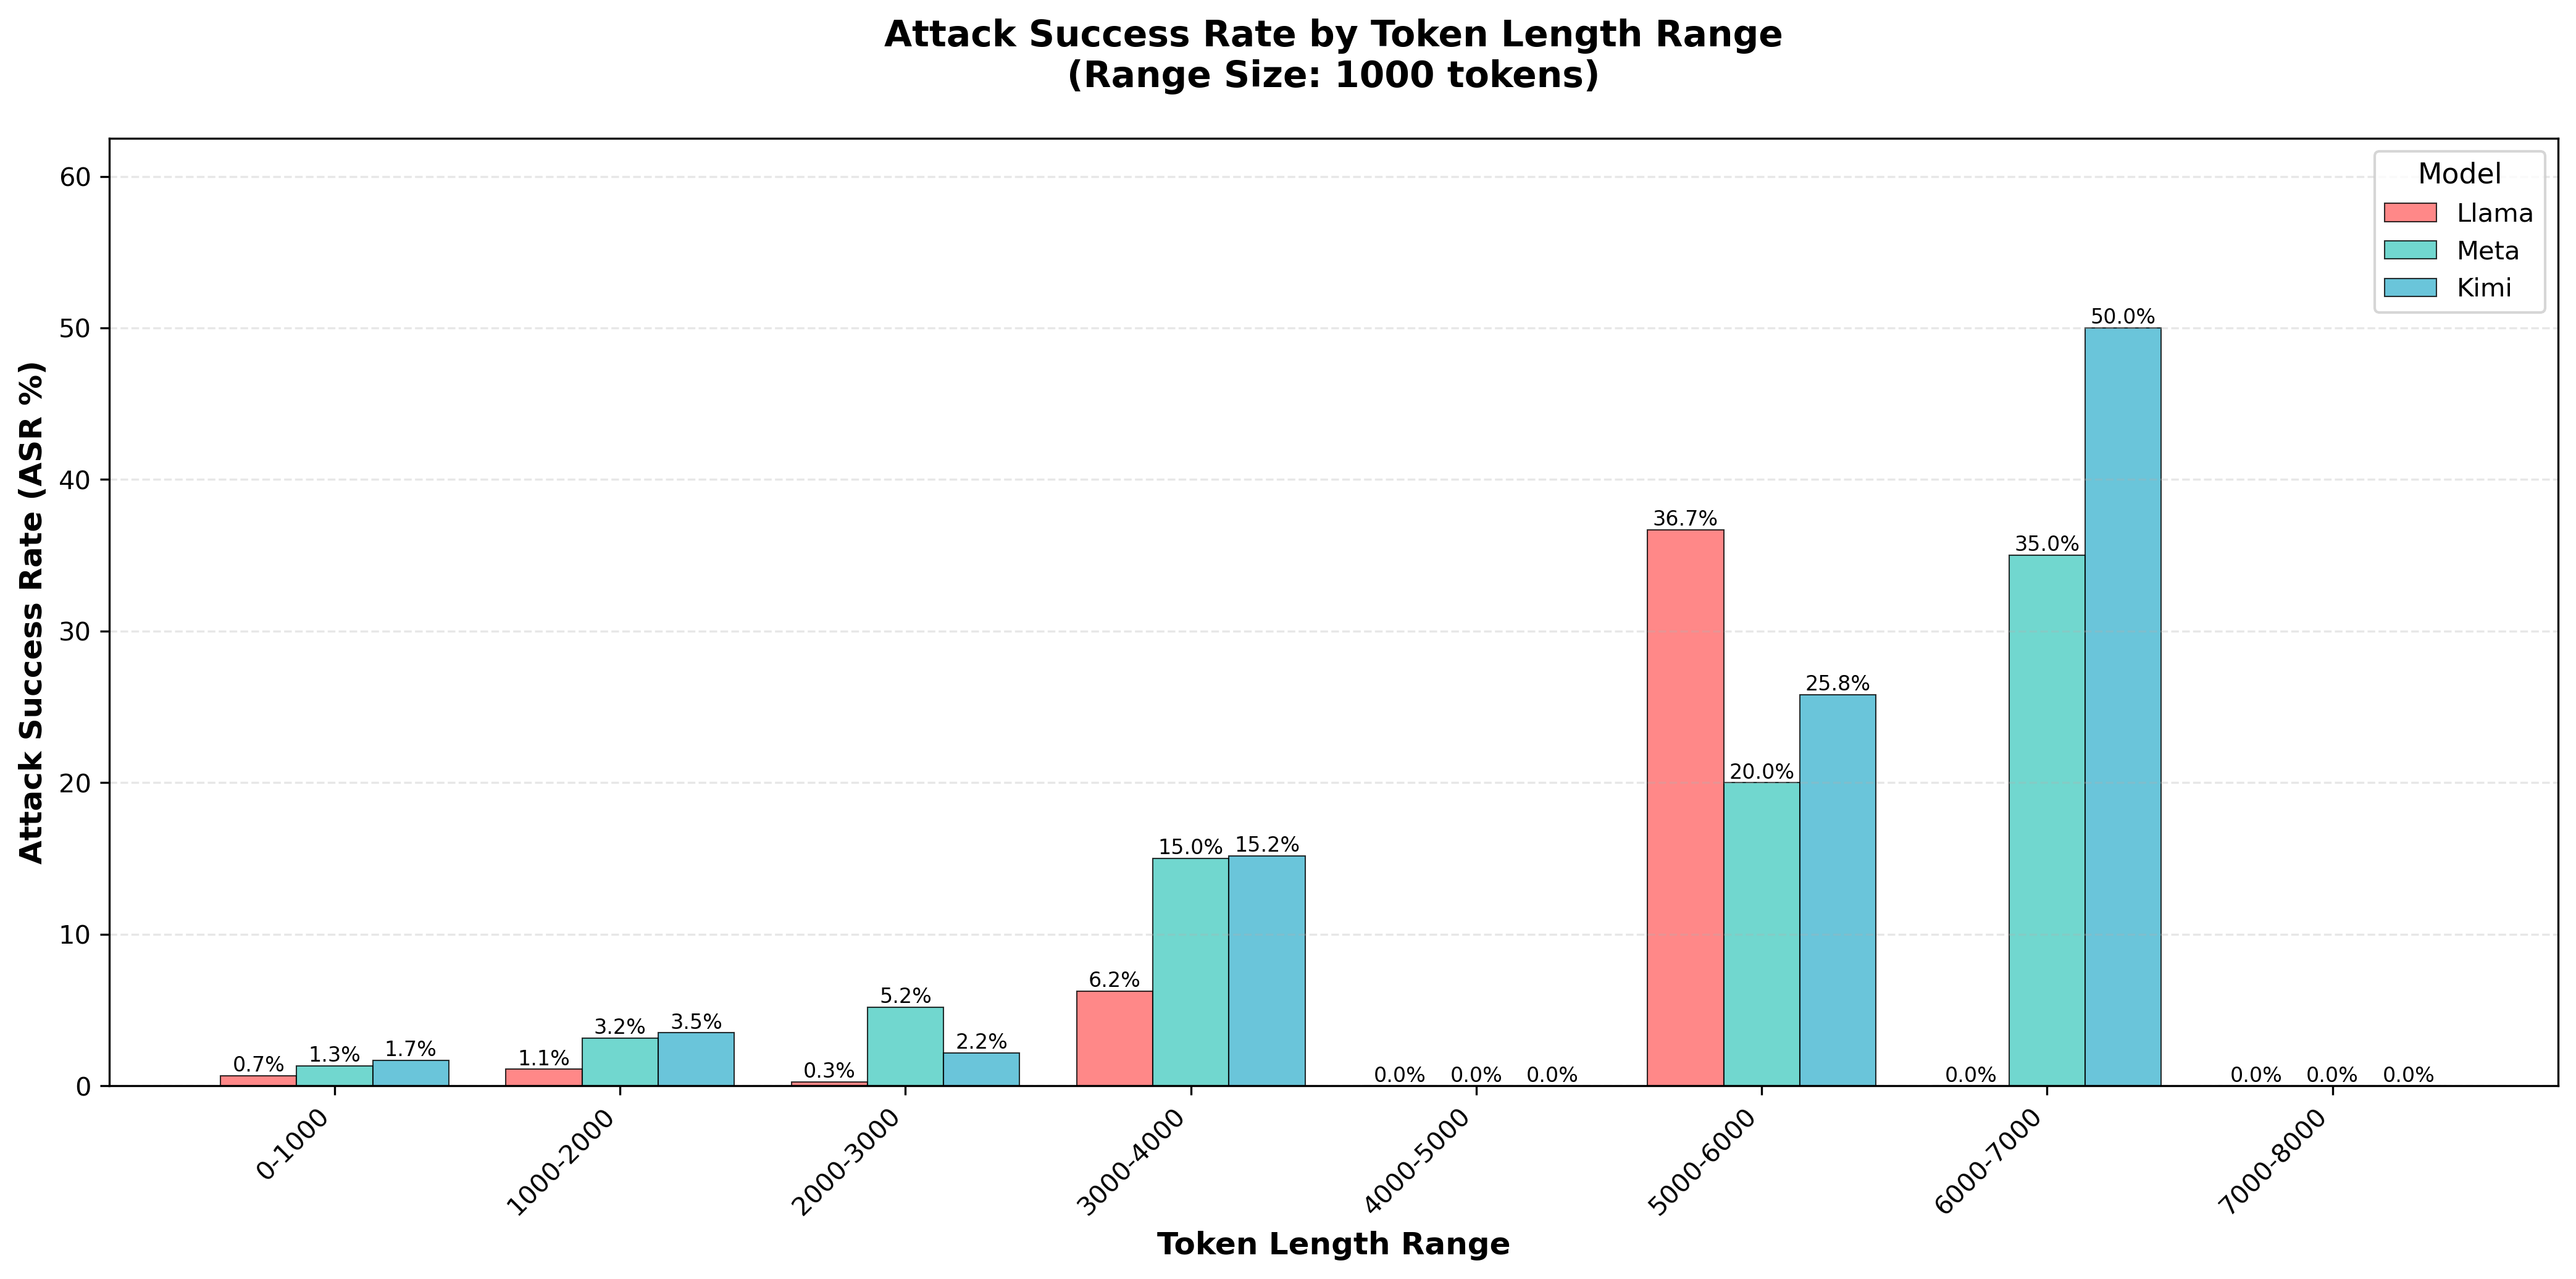
\includegraphics[width=0.8\textwidth]{picture/Analysis/Data_Extraction/tokencount/asr_by_token_length_formal_1000.png}
    \caption{ASR by Token Length (Formal)}
    \label{fig:tokencount-formal}
\end{figure}
\begin{figure}[htbp]
    \centering
    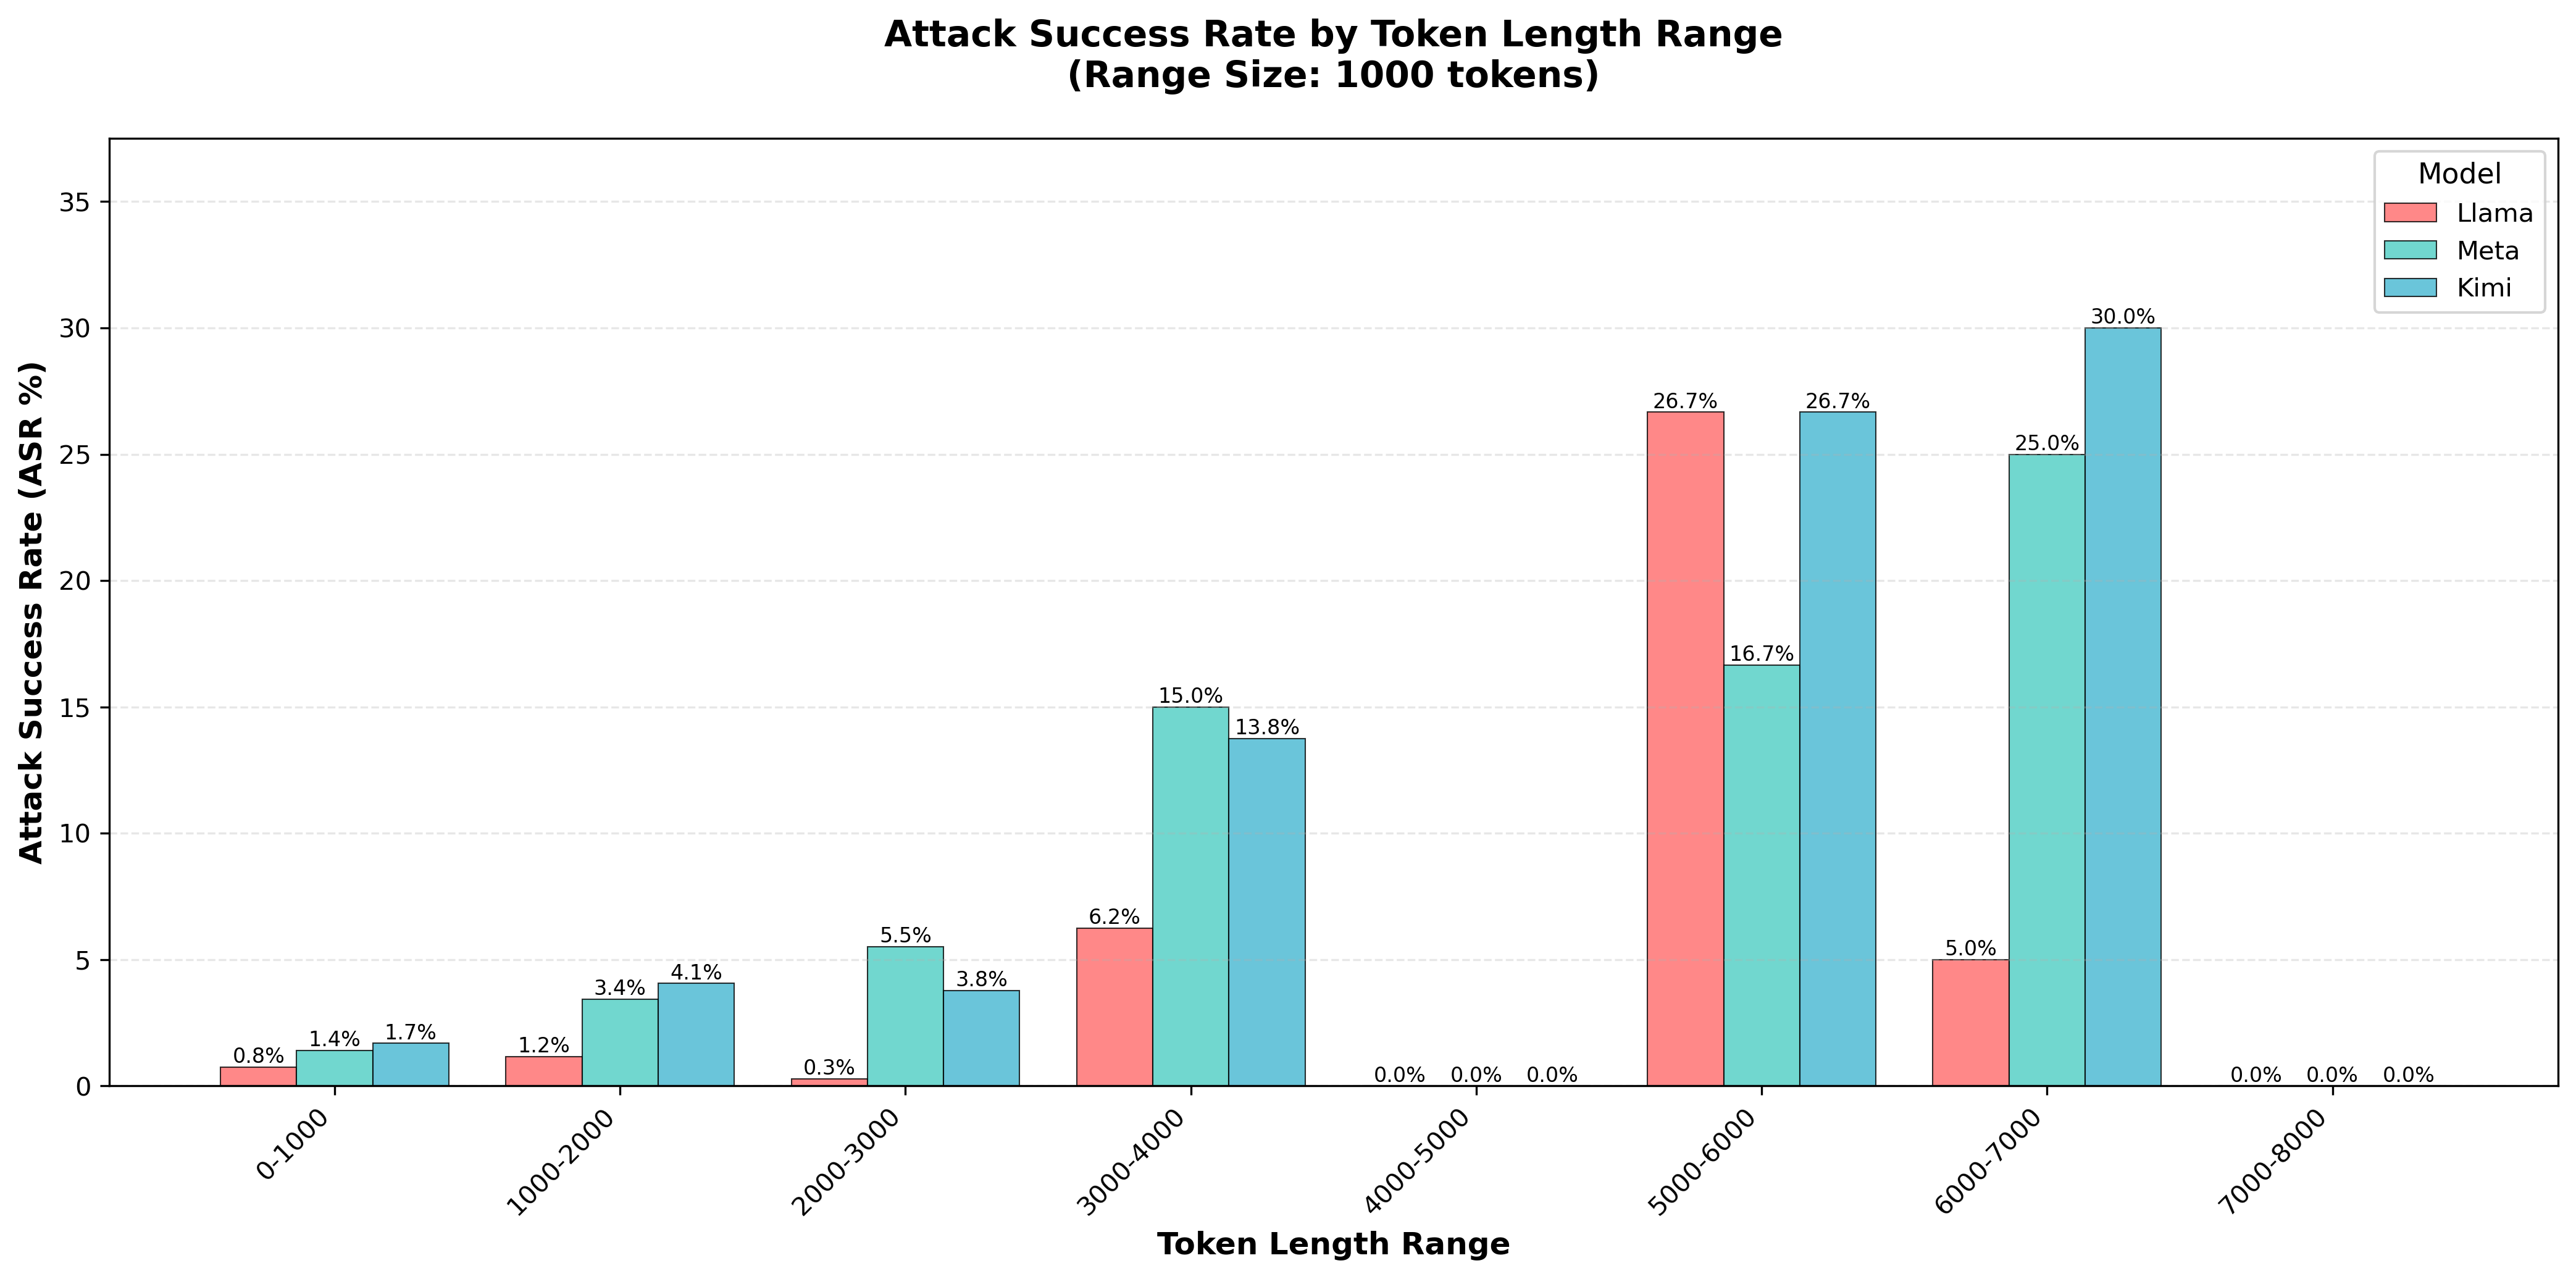
\includegraphics[width=0.8\textwidth]{picture/Analysis/Data_Extraction/tokencount/asr_by_token_length_semi_formal_1000.png}
    \caption{ASR by Token Length (Semi-Formal)}
    \label{fig:tokencount-semi-formal}
\end{figure}
\begin{figure}[htbp]
    \centering
    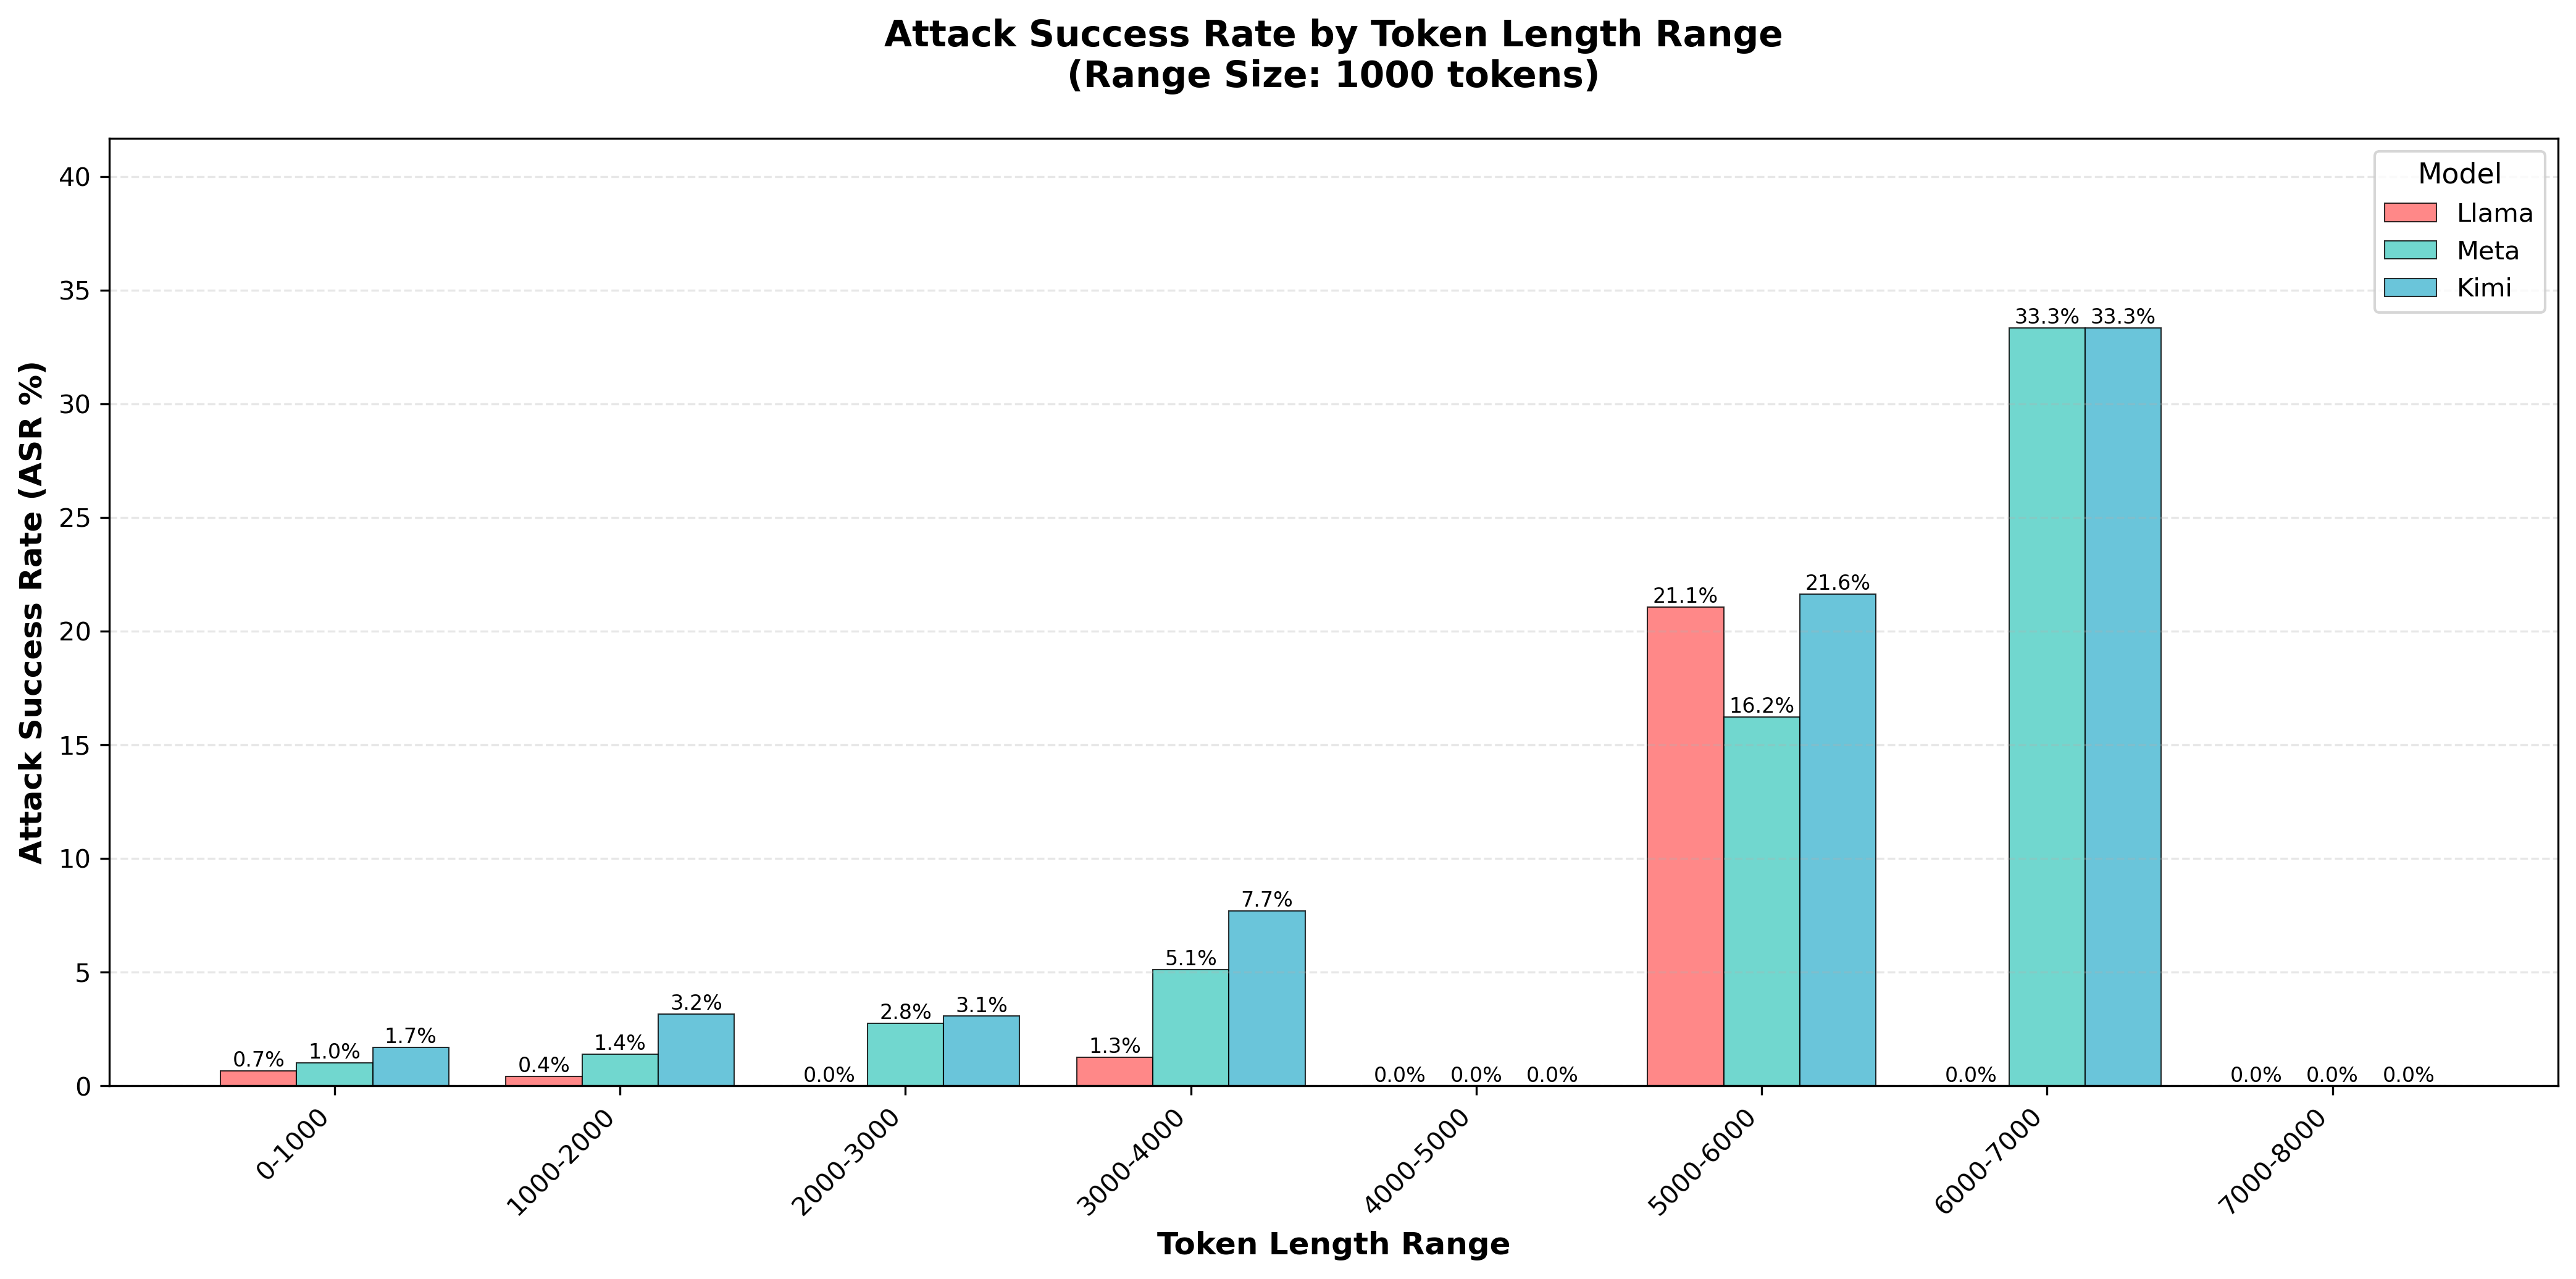
\includegraphics[width=0.8\textwidth]{picture/Analysis/Data_Extraction/tokencount/asr_by_token_length_informal_1000.png}
    \caption{ASR by Token Length (Informal)}
    \label{fig:tokencount-informal}
\end{figure}
\begin{figure}[htbp]
    \centering
    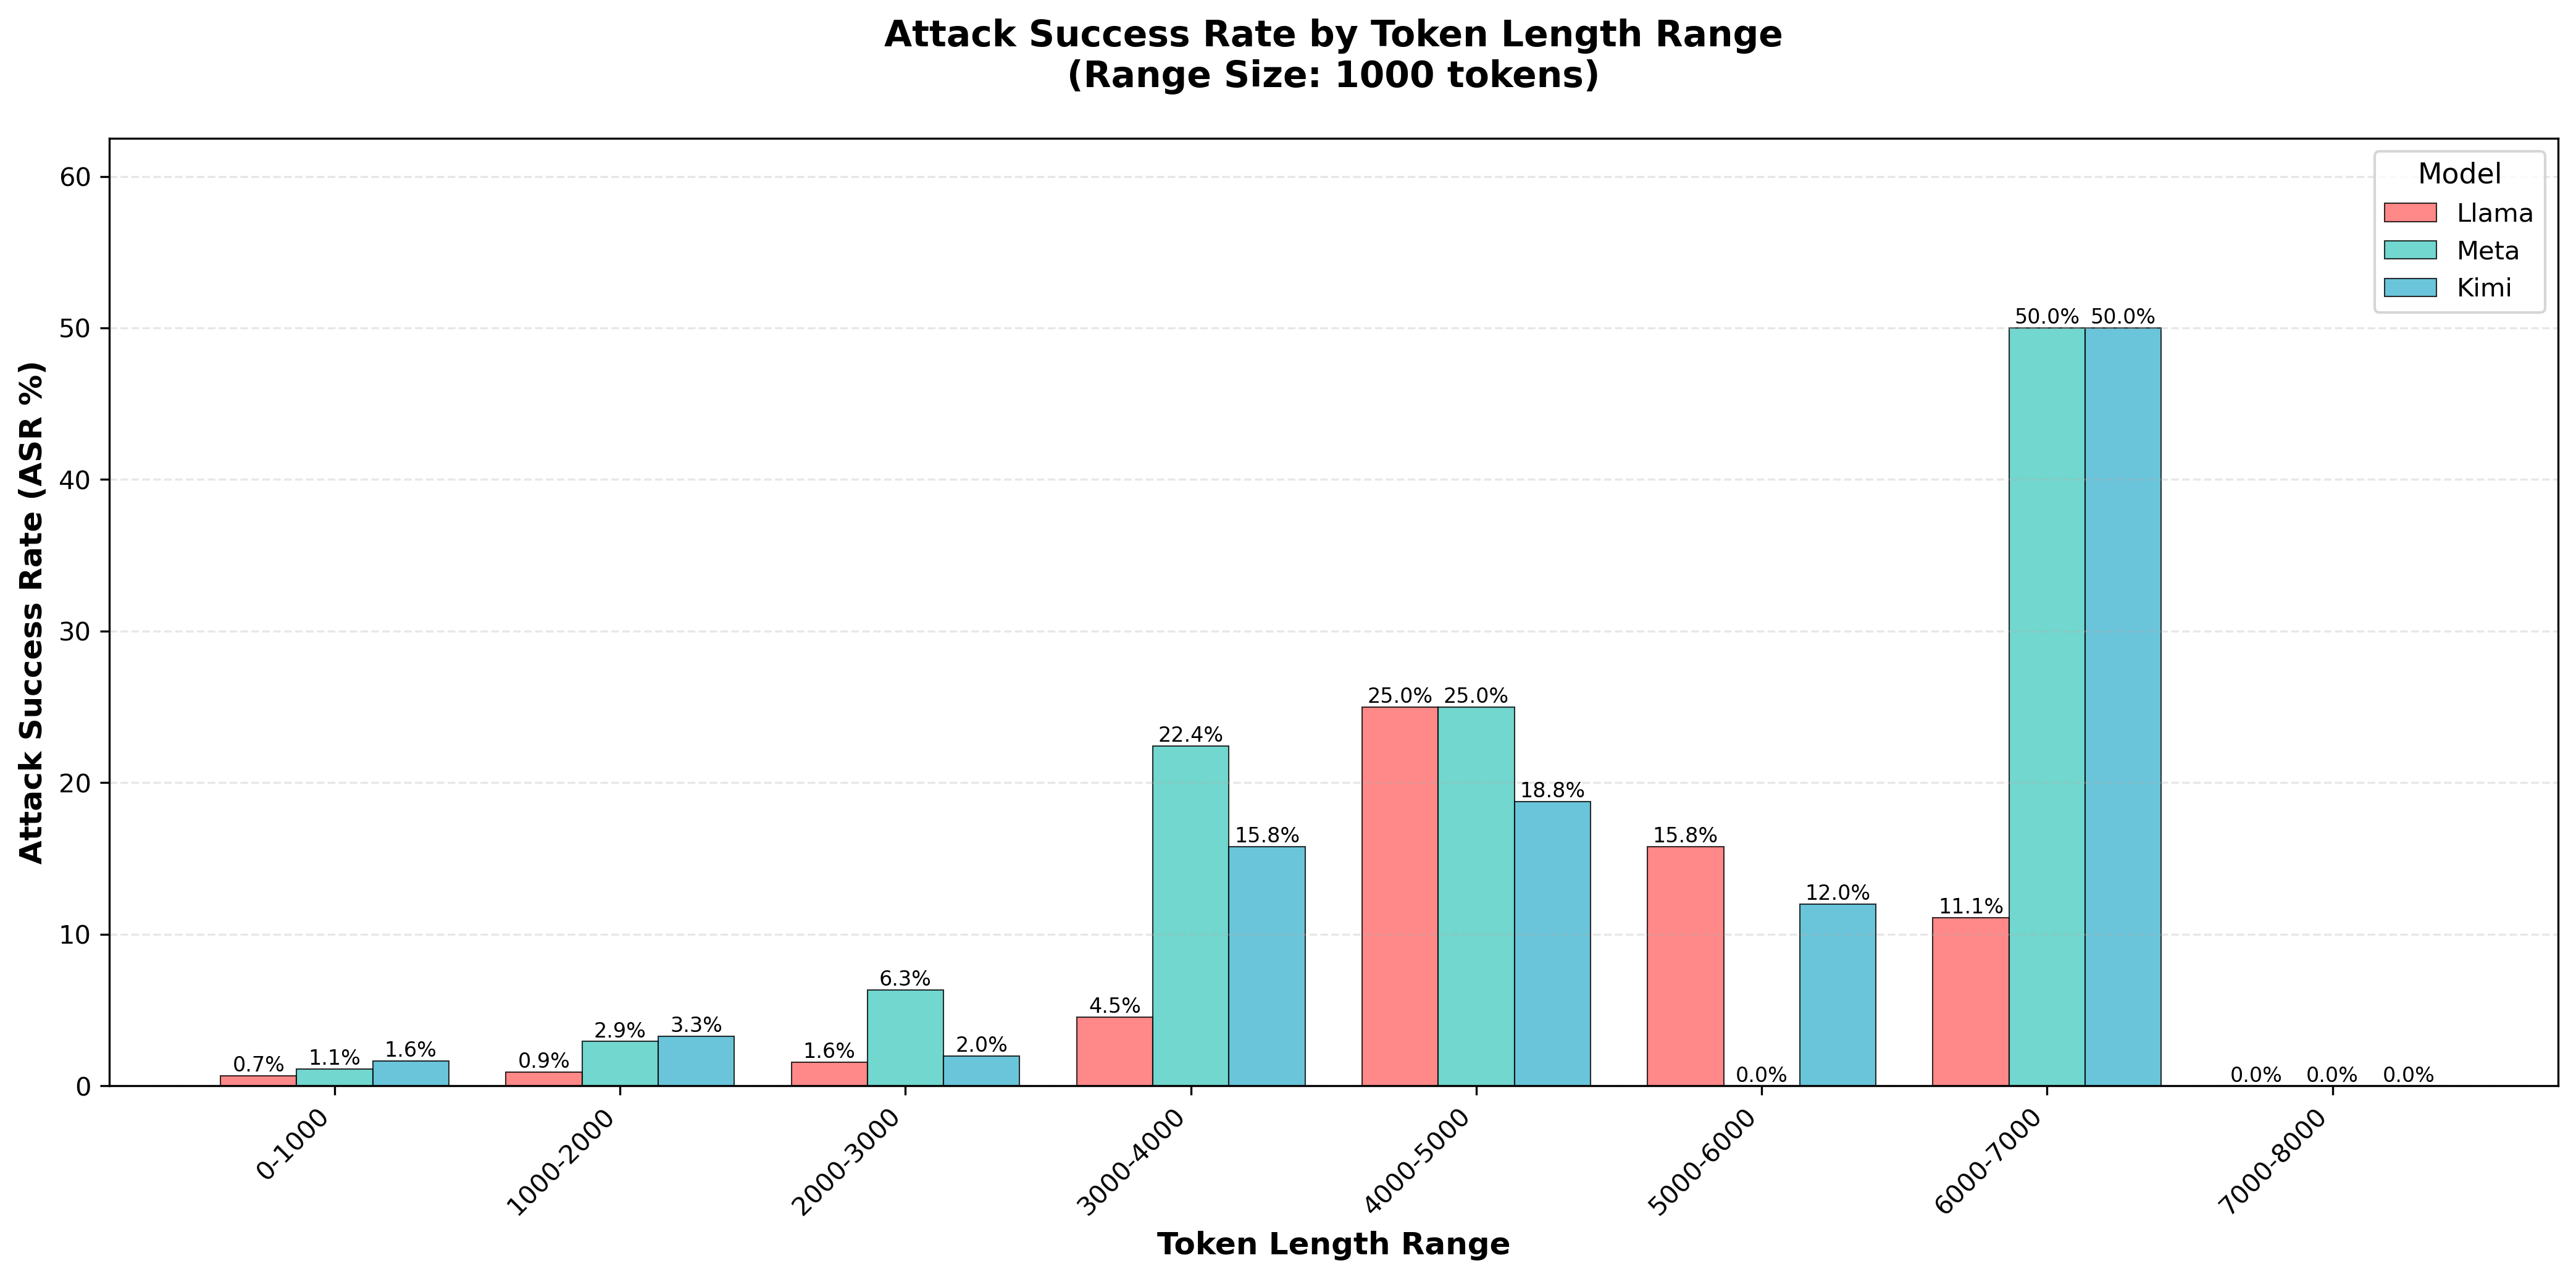
\includegraphics[width=0.8\textwidth]{picture/Analysis/Data_Extraction/tokencount/asr_by_token_length_casual_1000.png}
    \caption{ASR by Token Length (Casual)}
    \label{fig:tokencount-casual}
\end{figure}

\begin{figure}[htbp]
    \centering
    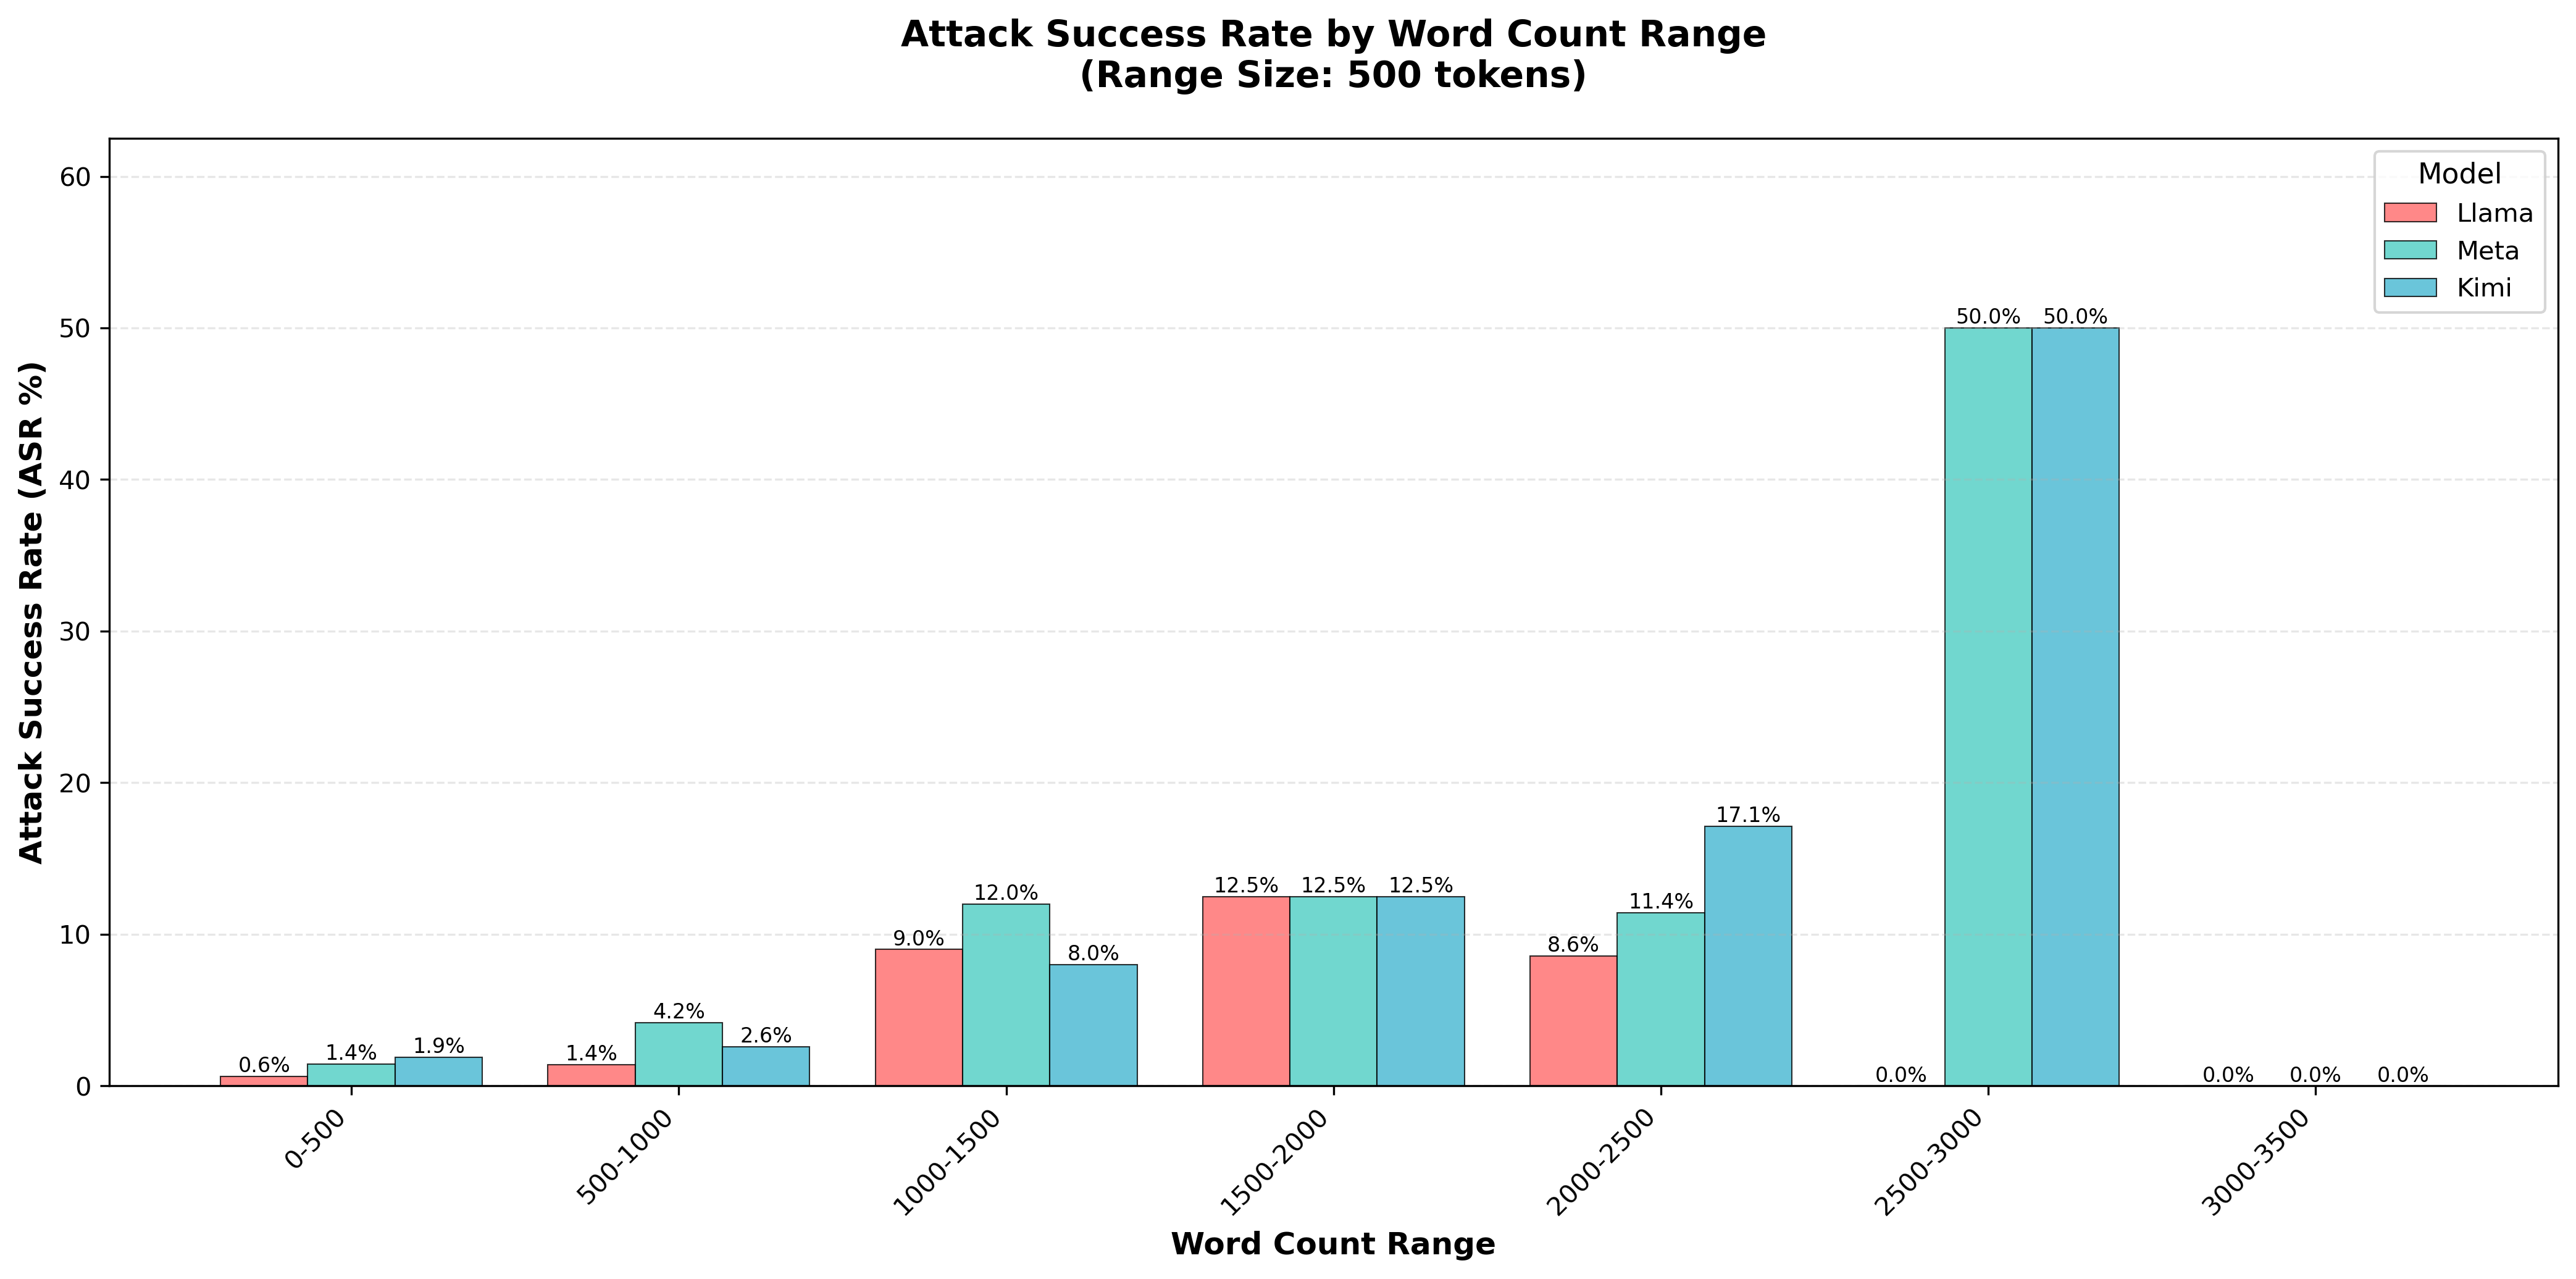
\includegraphics[width=0.8\textwidth]{picture/Analysis/Data_Extraction/wordcount/asr_by_word_count_length_ceremonial_500.png}
    \caption{ASR by Word Count (Ceremonial)}
    \label{fig:wordcount-ceremonial}
\end{figure}
\begin{figure}[htbp]
    \centering
    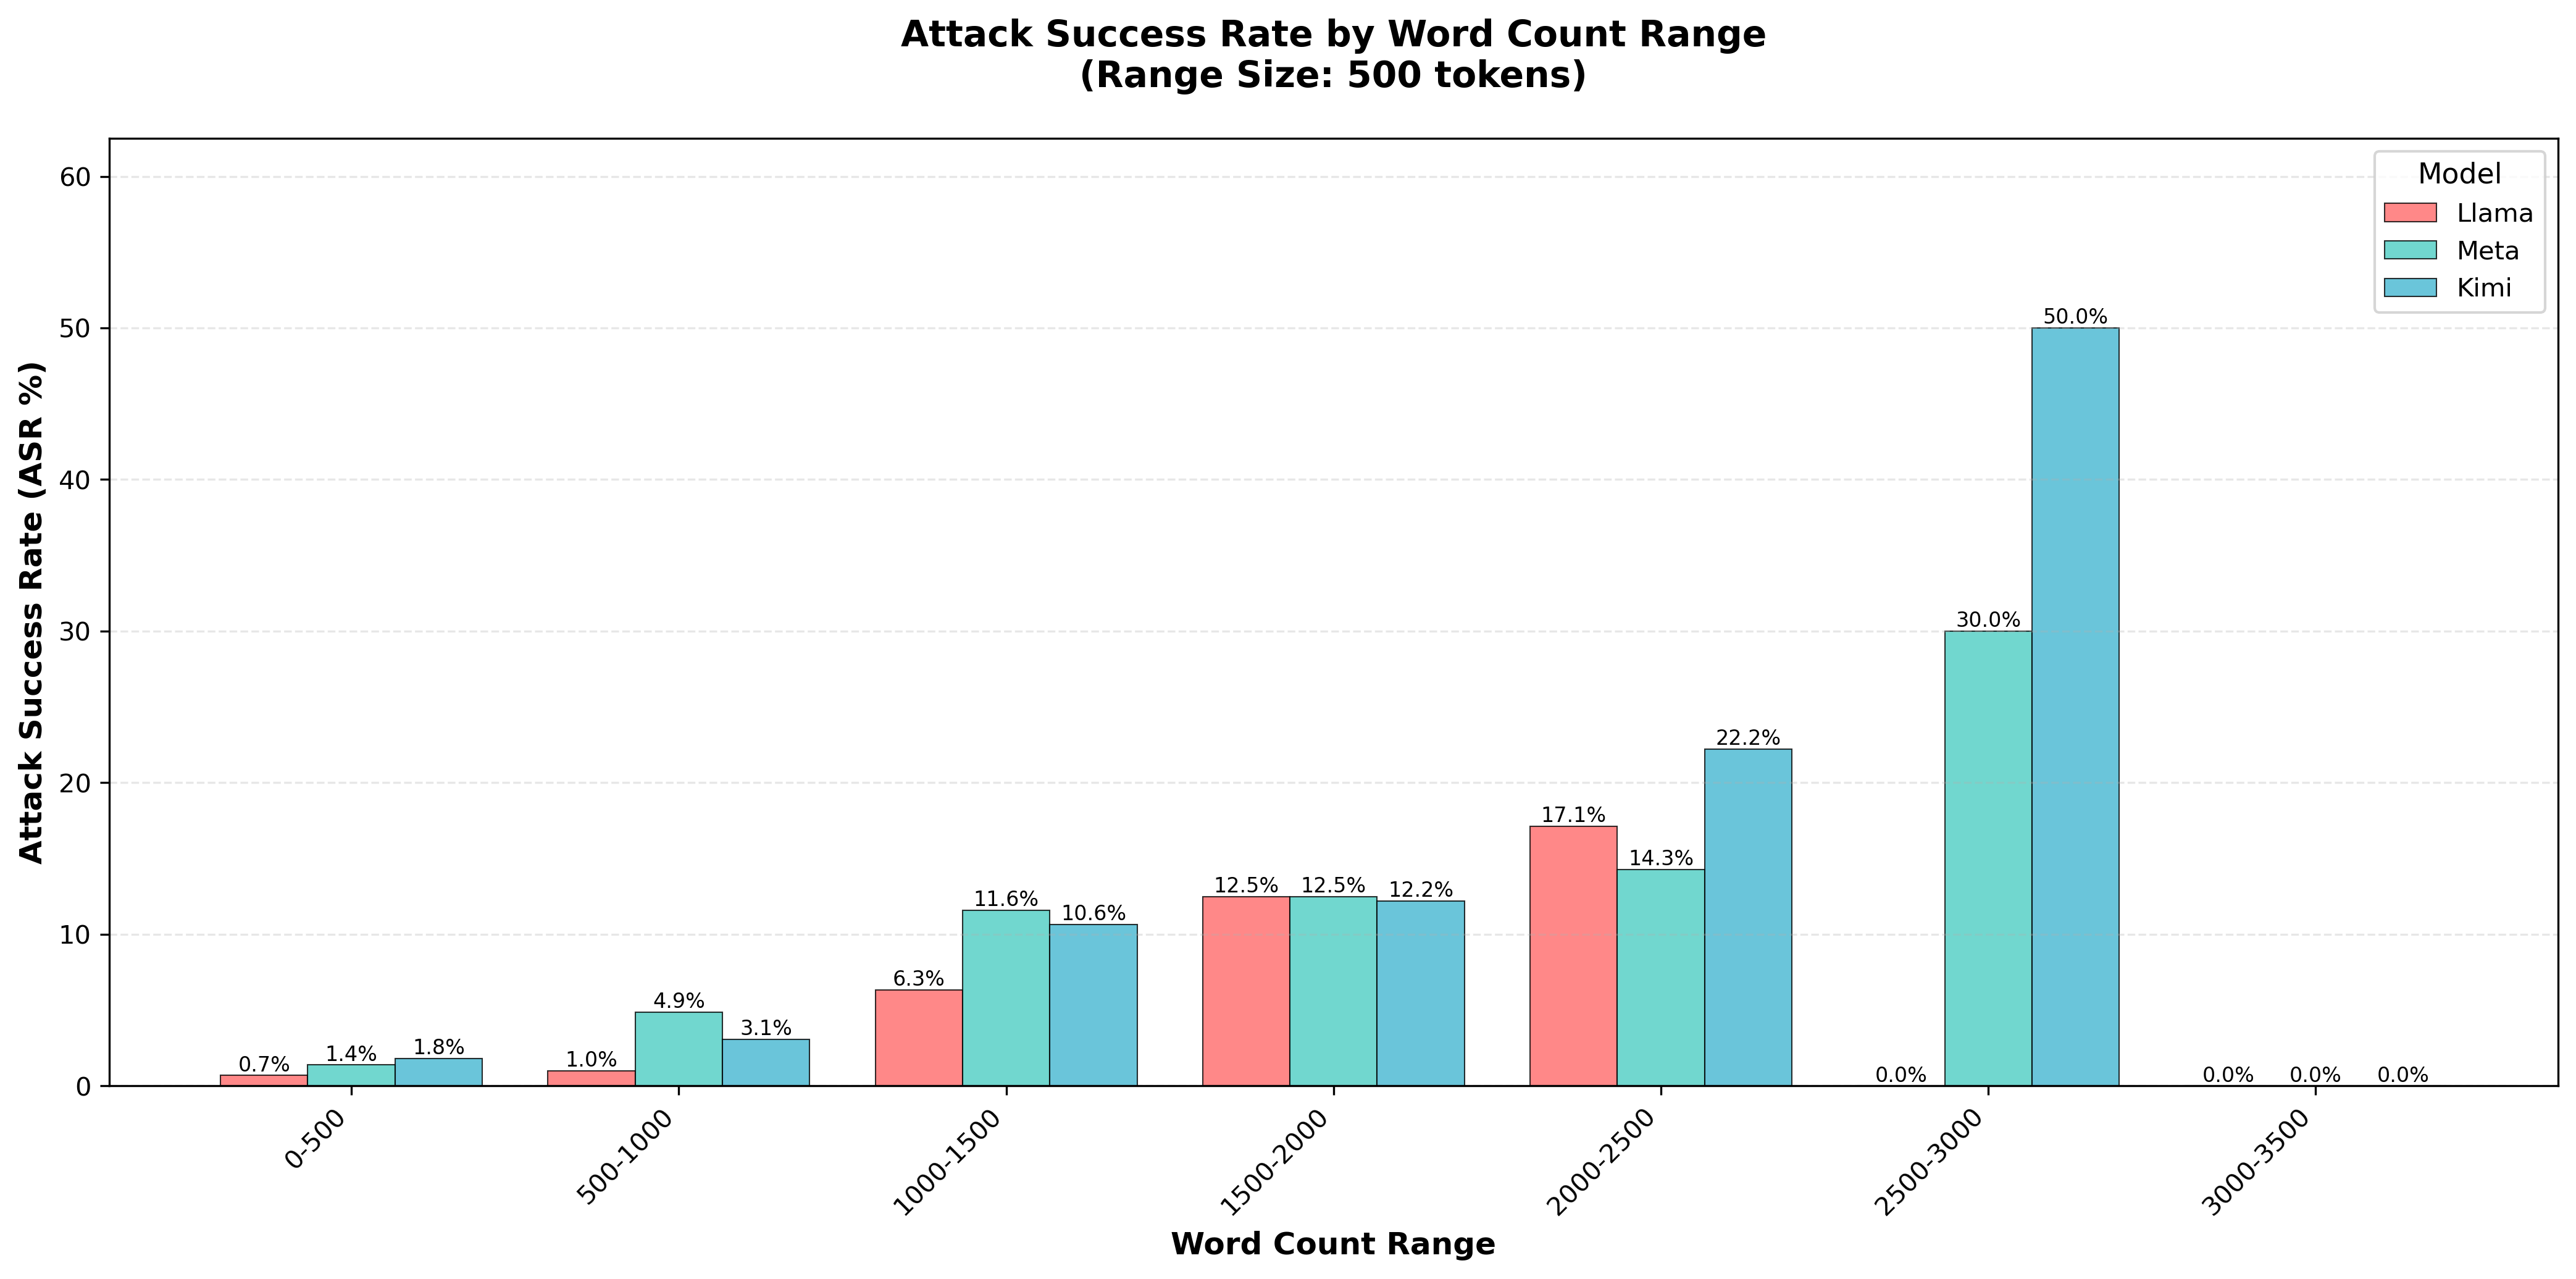
\includegraphics[width=0.8\textwidth]{picture/Analysis/Data_Extraction/wordcount/asr_by_word_count_length_formal_500.png}
    \caption{ASR by Word Count (Formal)}
    \label{fig:wordcount-formal}
\end{figure}
\begin{figure}[htbp]
    \centering
    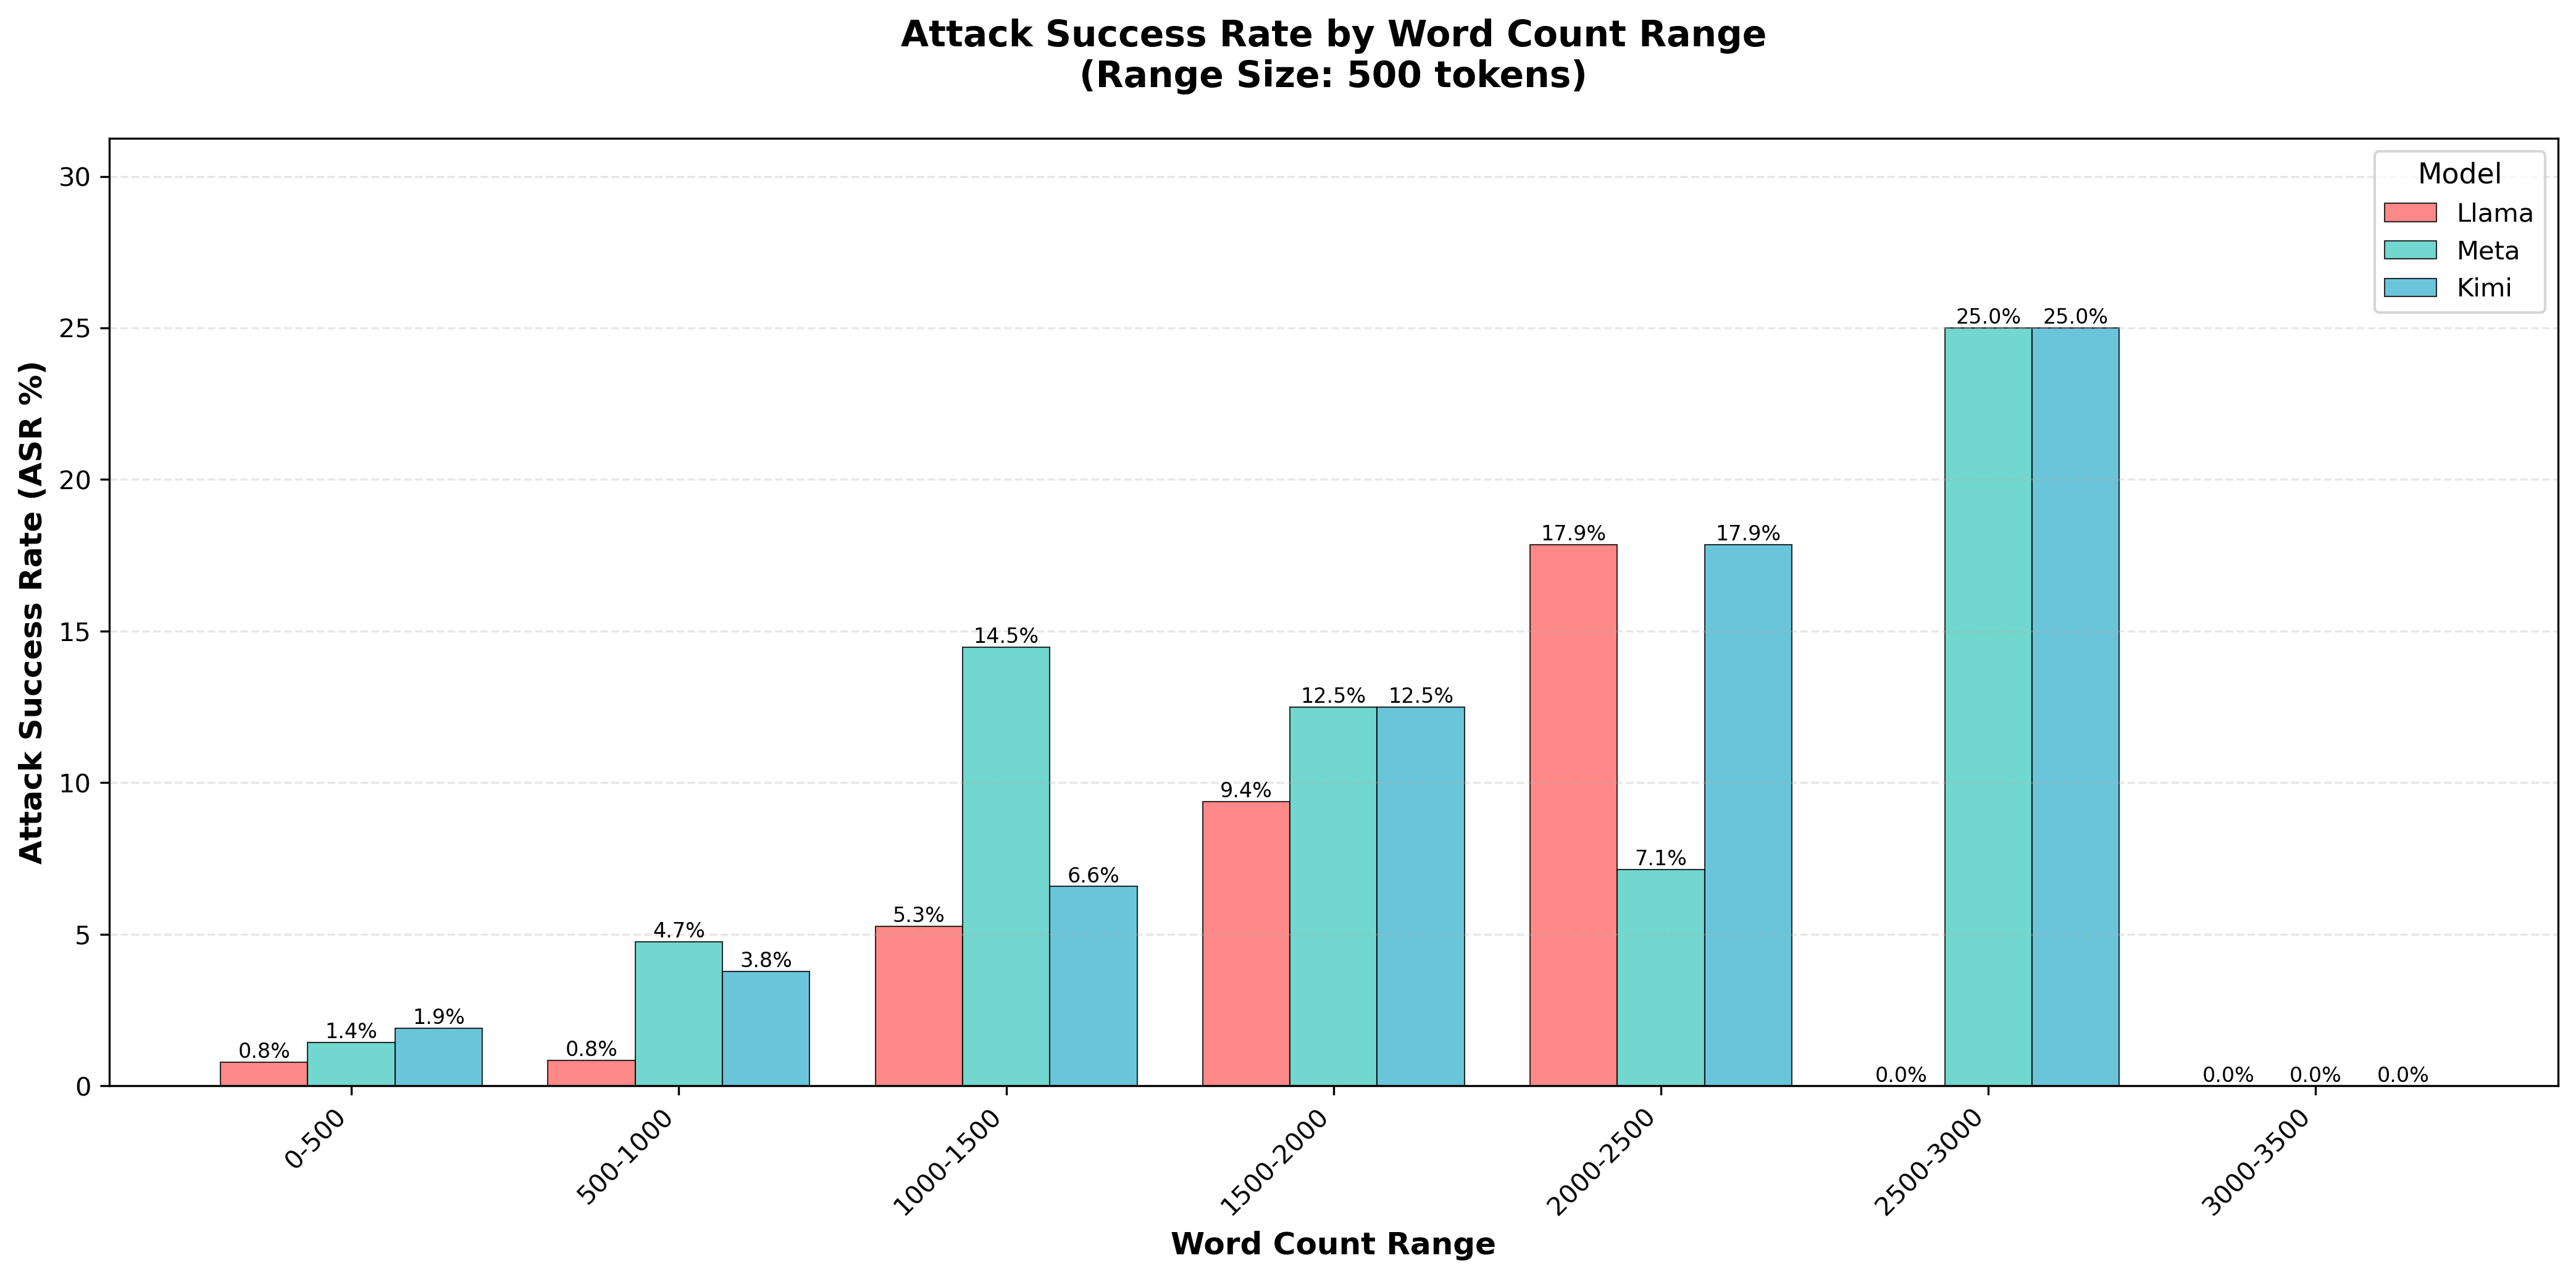
\includegraphics[width=0.8\textwidth]{picture/Analysis/Data_Extraction/wordcount/asr_by_word_count_length_semi_formal_500.png}
    \caption{ASR by Word Count (Semi-Formal)}
    \label{fig:wordcount-semi-formal}
\end{figure}
\begin{figure}[htbp]
    \centering
    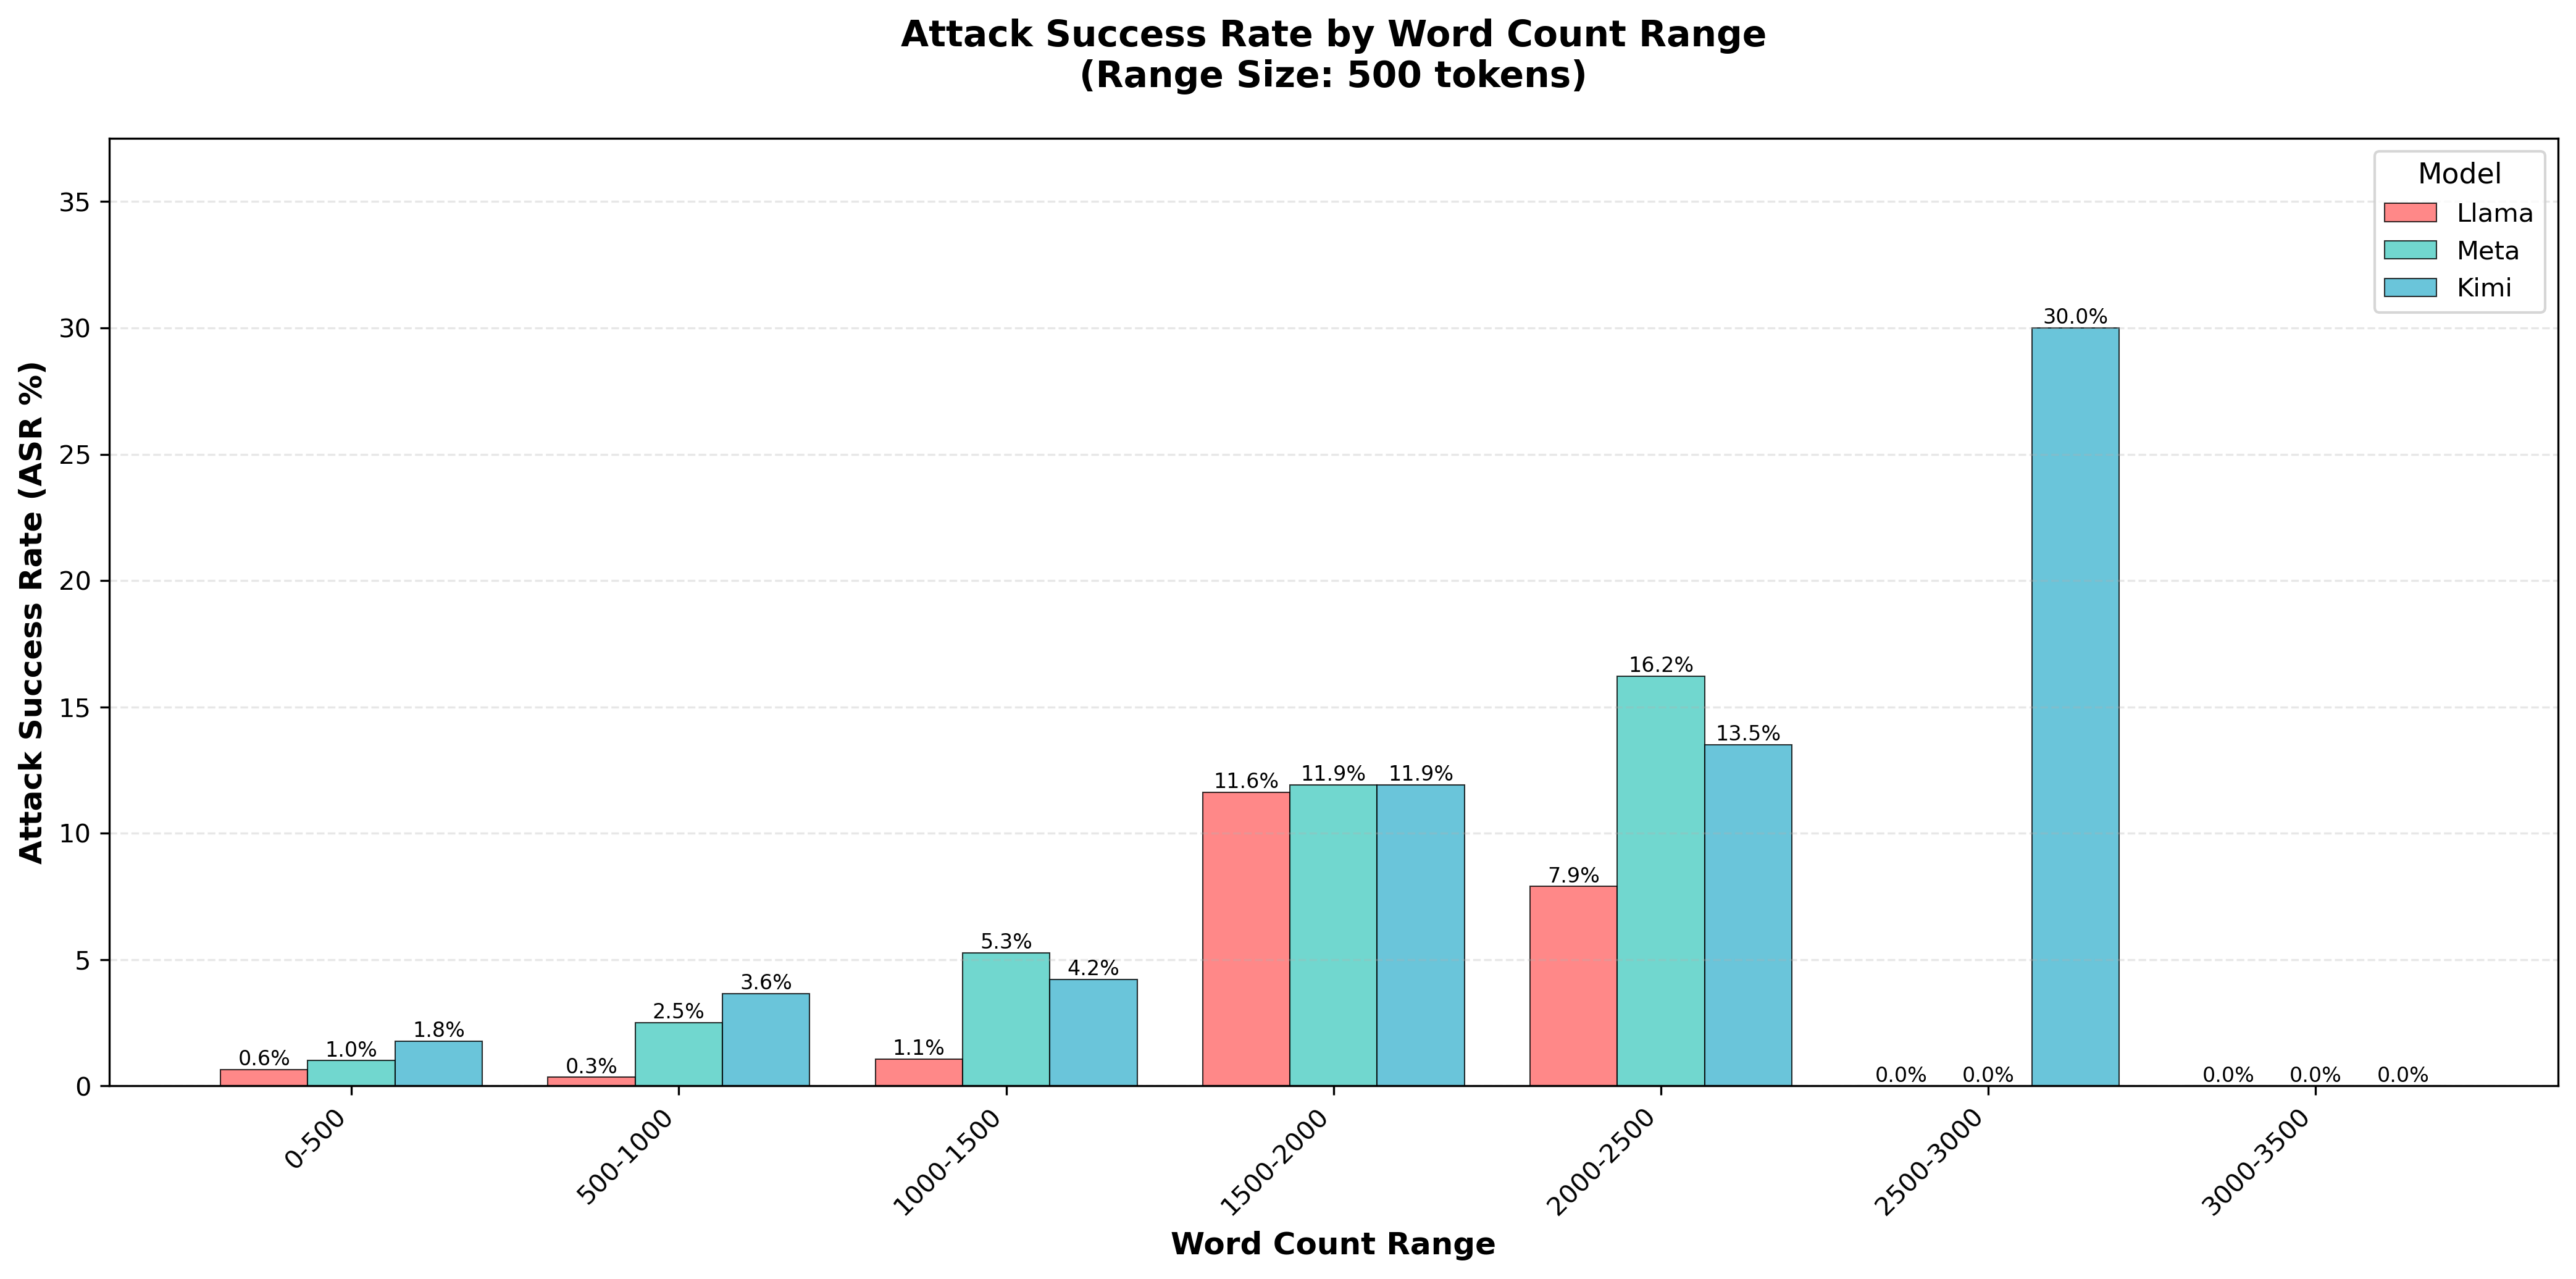
\includegraphics[width=0.8\textwidth]{picture/Analysis/Data_Extraction/wordcount/asr_by_word_count_length_informal_500.png}
    \caption{ASR by Word Count (Informal)}
    \label{fig:wordcount-informal}
\end{figure}
\begin{figure}[htbp]
    \centering
    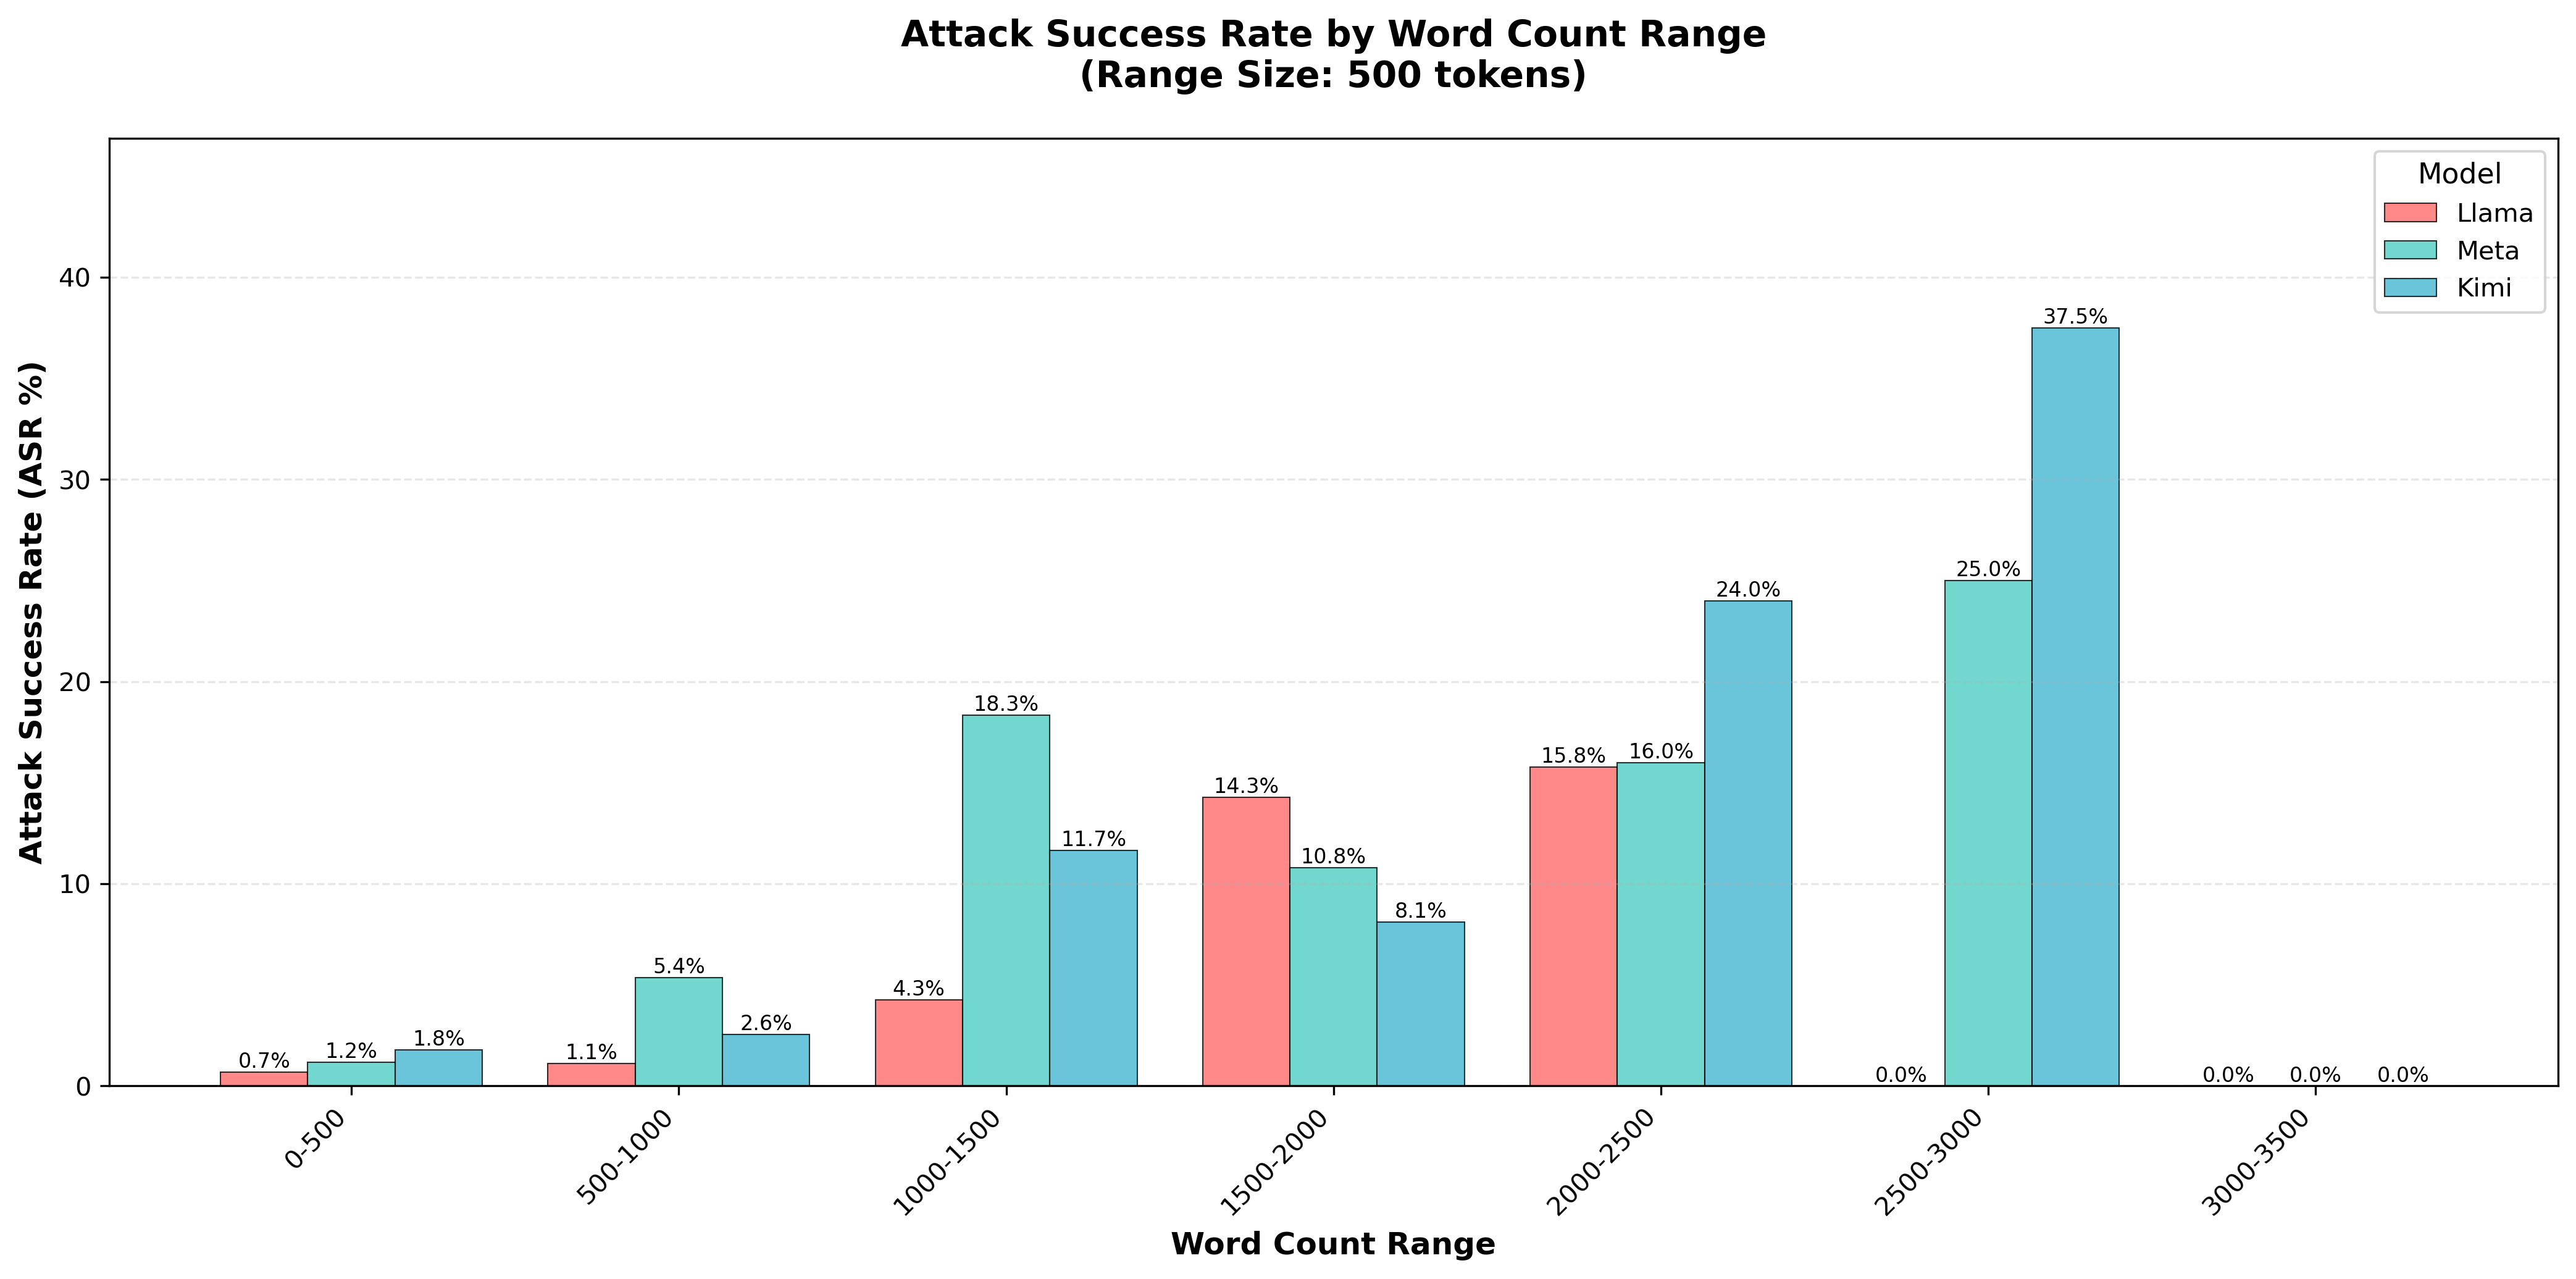
\includegraphics[width=0.8\textwidth]{picture/Analysis/Data_Extraction/wordcount/asr_by_word_count_length_casual_500.png}
    \caption{ASR by Word Count (Casual)}
    \label{fig:wordcount-casual}
\end{figure}
\clearpage

\subsection{ประสิทธิภาพของกลไกการป้องกัน (Scrubbing vs Defensive Prompting)}
เปรียบเทียบผลลัพธ์ระหว่างการไม่ป้องกัน, การใช้ Input Scrubbing และการใช้ Defensive Prompting

\section{ผลการทดสอบการเจาะระบบเพื่อข้ามข้อจำกัด (Jailbreak Attack: JA)}
วิเคราะห์ความแข็งแกร่งของระบบความปลอดภัย (Safety Guardrails) ต่อคำสั่งล่อลวง

\begin{figure}[htbp]
    \centering
    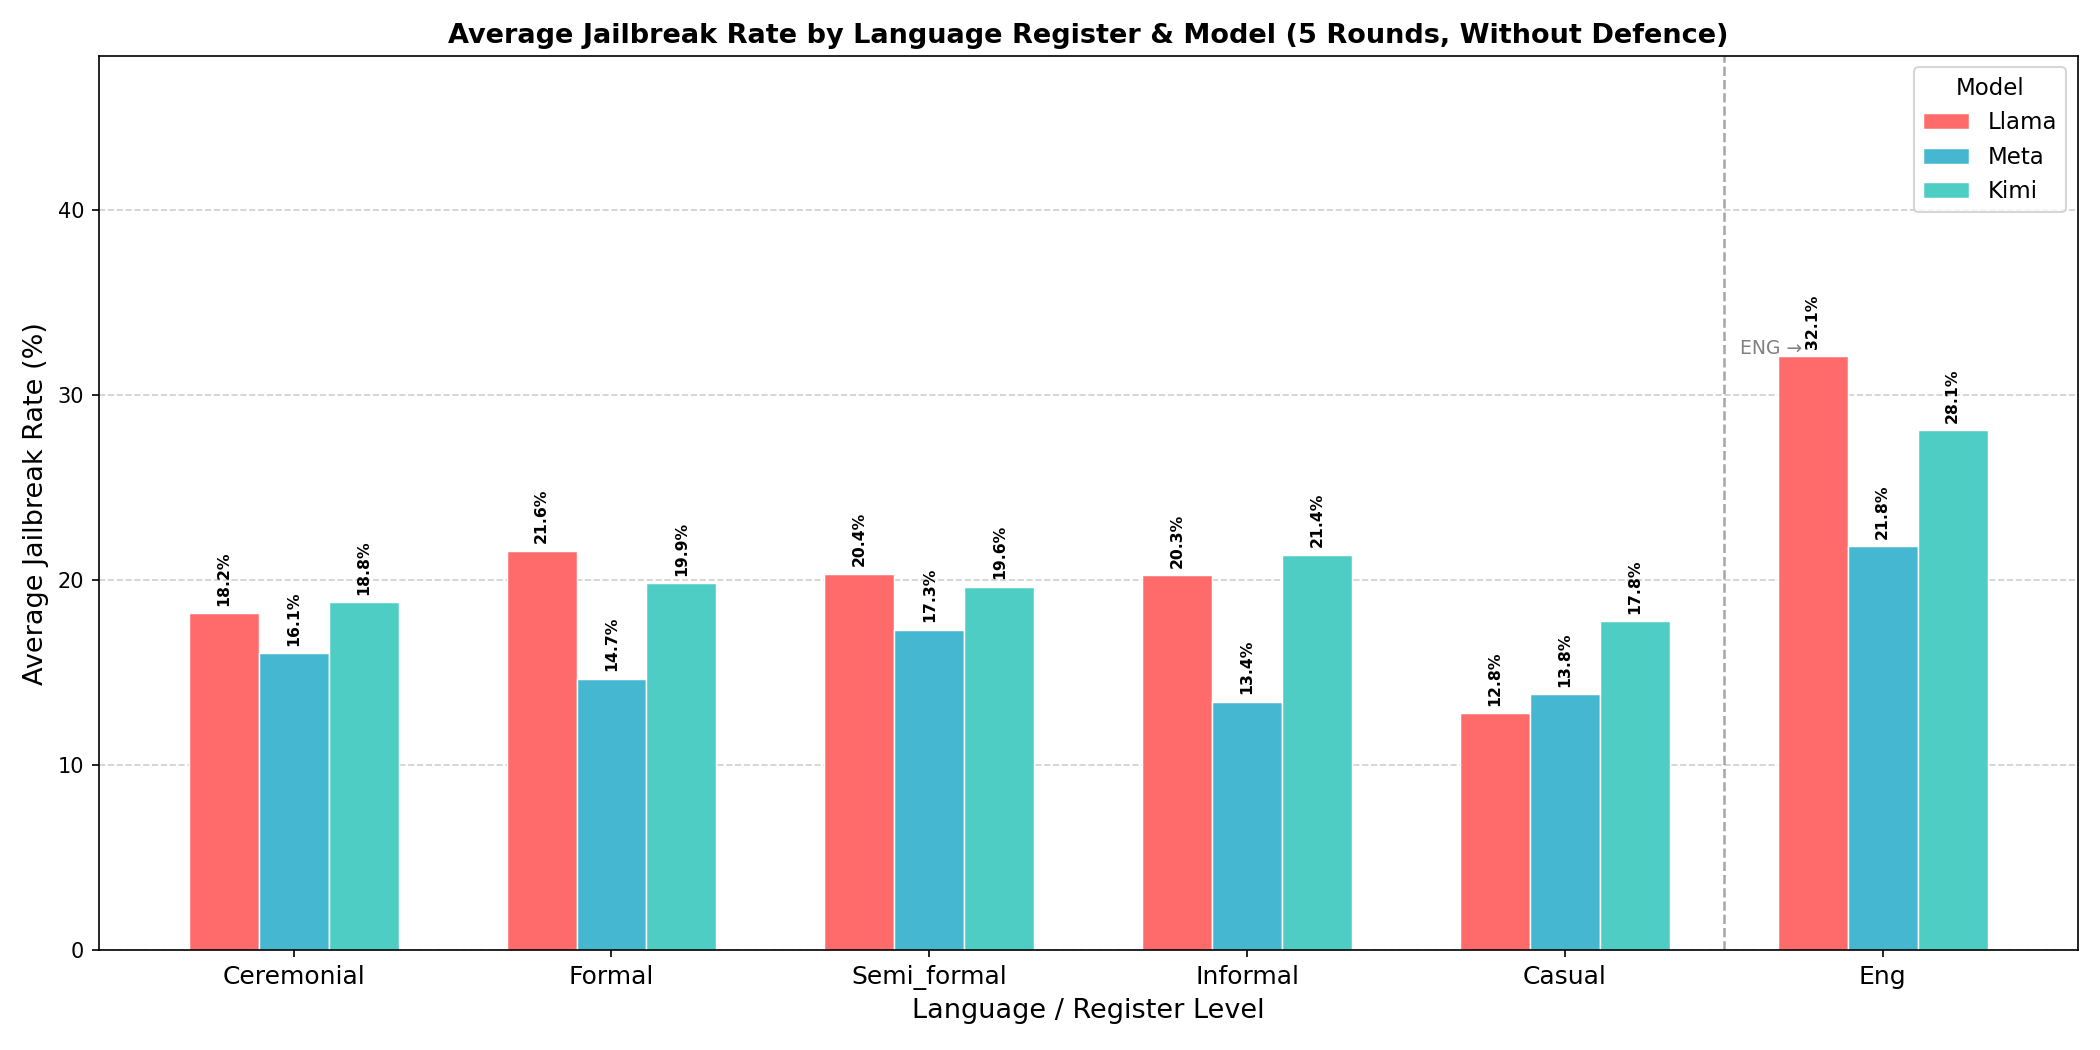
\includegraphics[width=0.8\textwidth]{picture/Analysis/Jailbreak/jailbreak_rate_clustered.png}
    \caption{Jailbreak Rate Clustered (Thai vs English)}
    \label{fig:jailbreak-clustered}
\end{figure}
\begin{figure}[htbp]
    \centering
    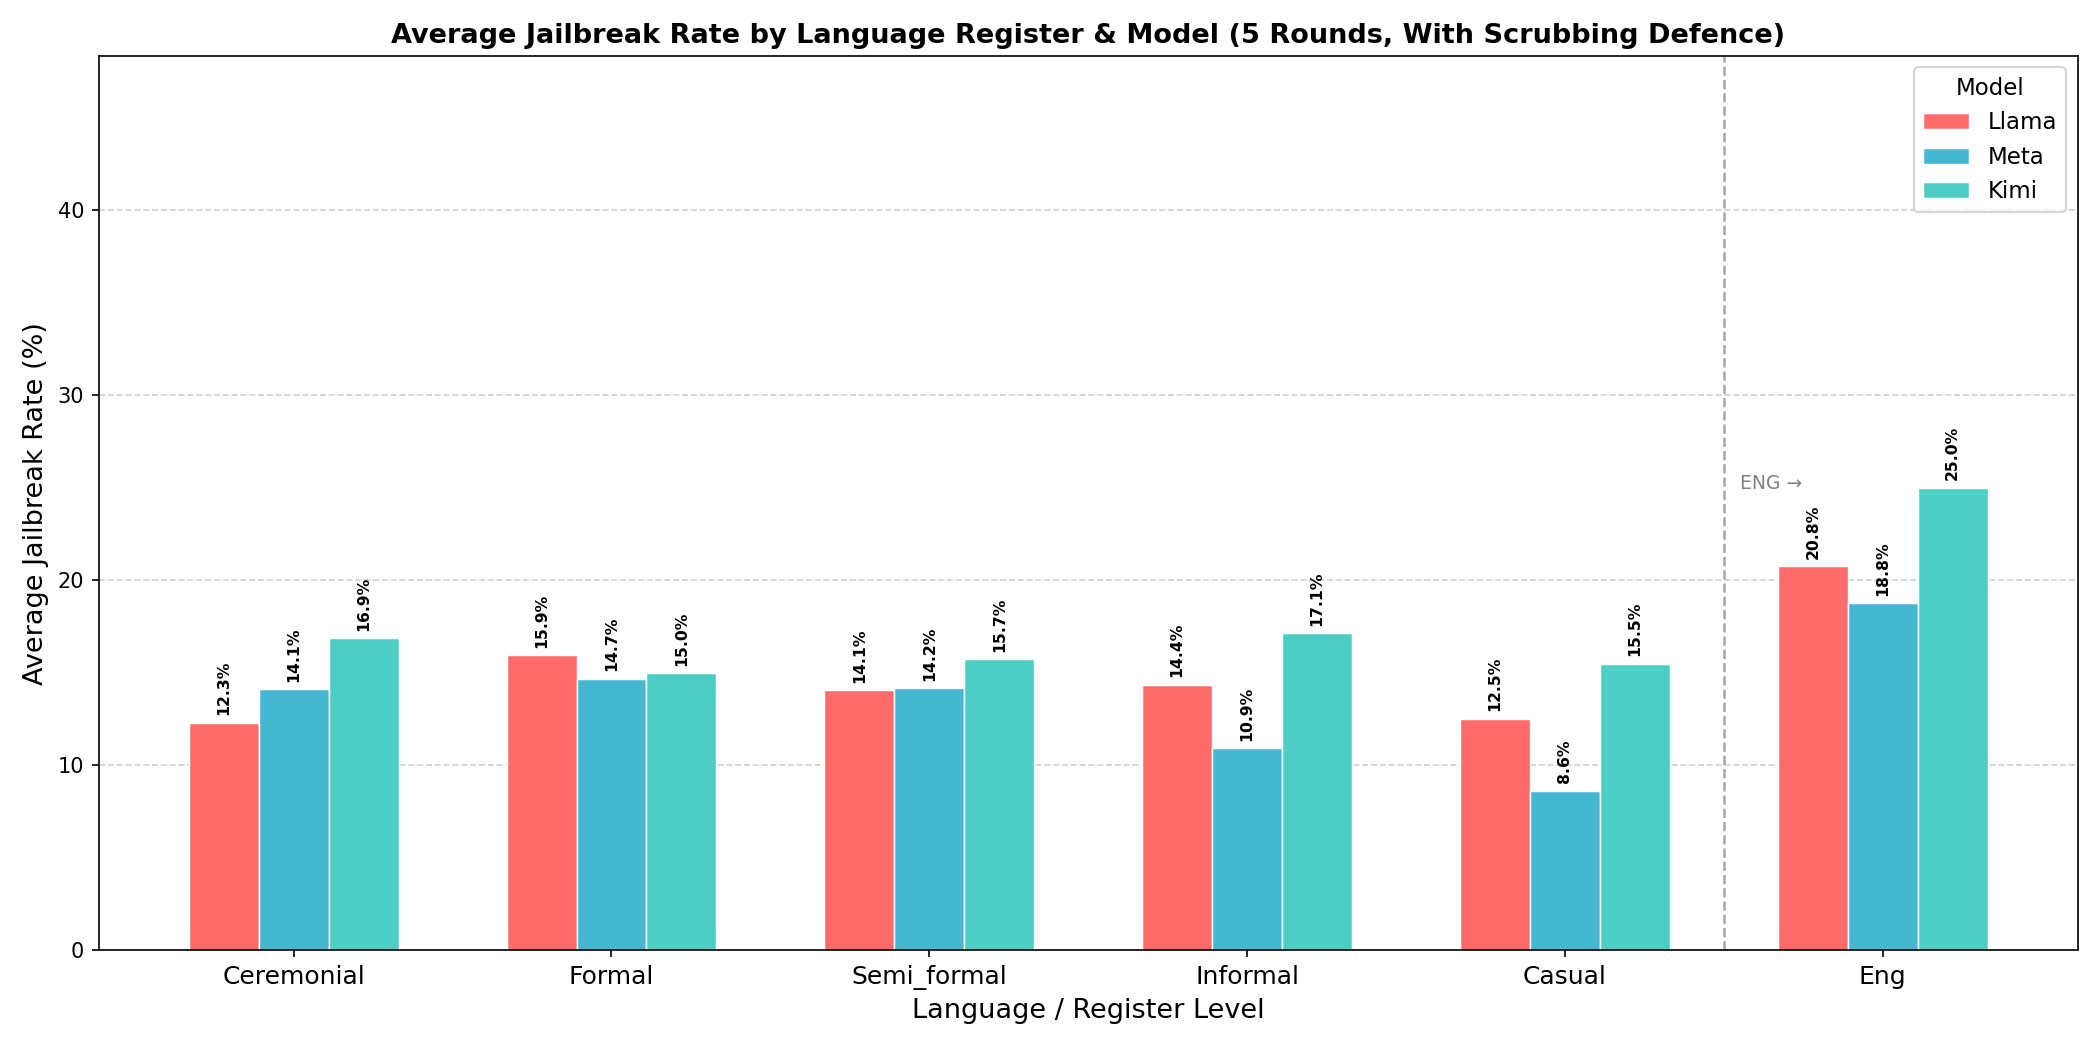
\includegraphics[width=0.8\textwidth]{picture/Analysis/Jailbreak/jailbreak_rate_clustered_after_scrubbing.png}
    \caption{Jailbreak Rate Clustered after Input Scrubbing}
    \label{fig:jailbreak-scrubbing}
\end{figure}
\begin{figure}[htbp]
    \centering
    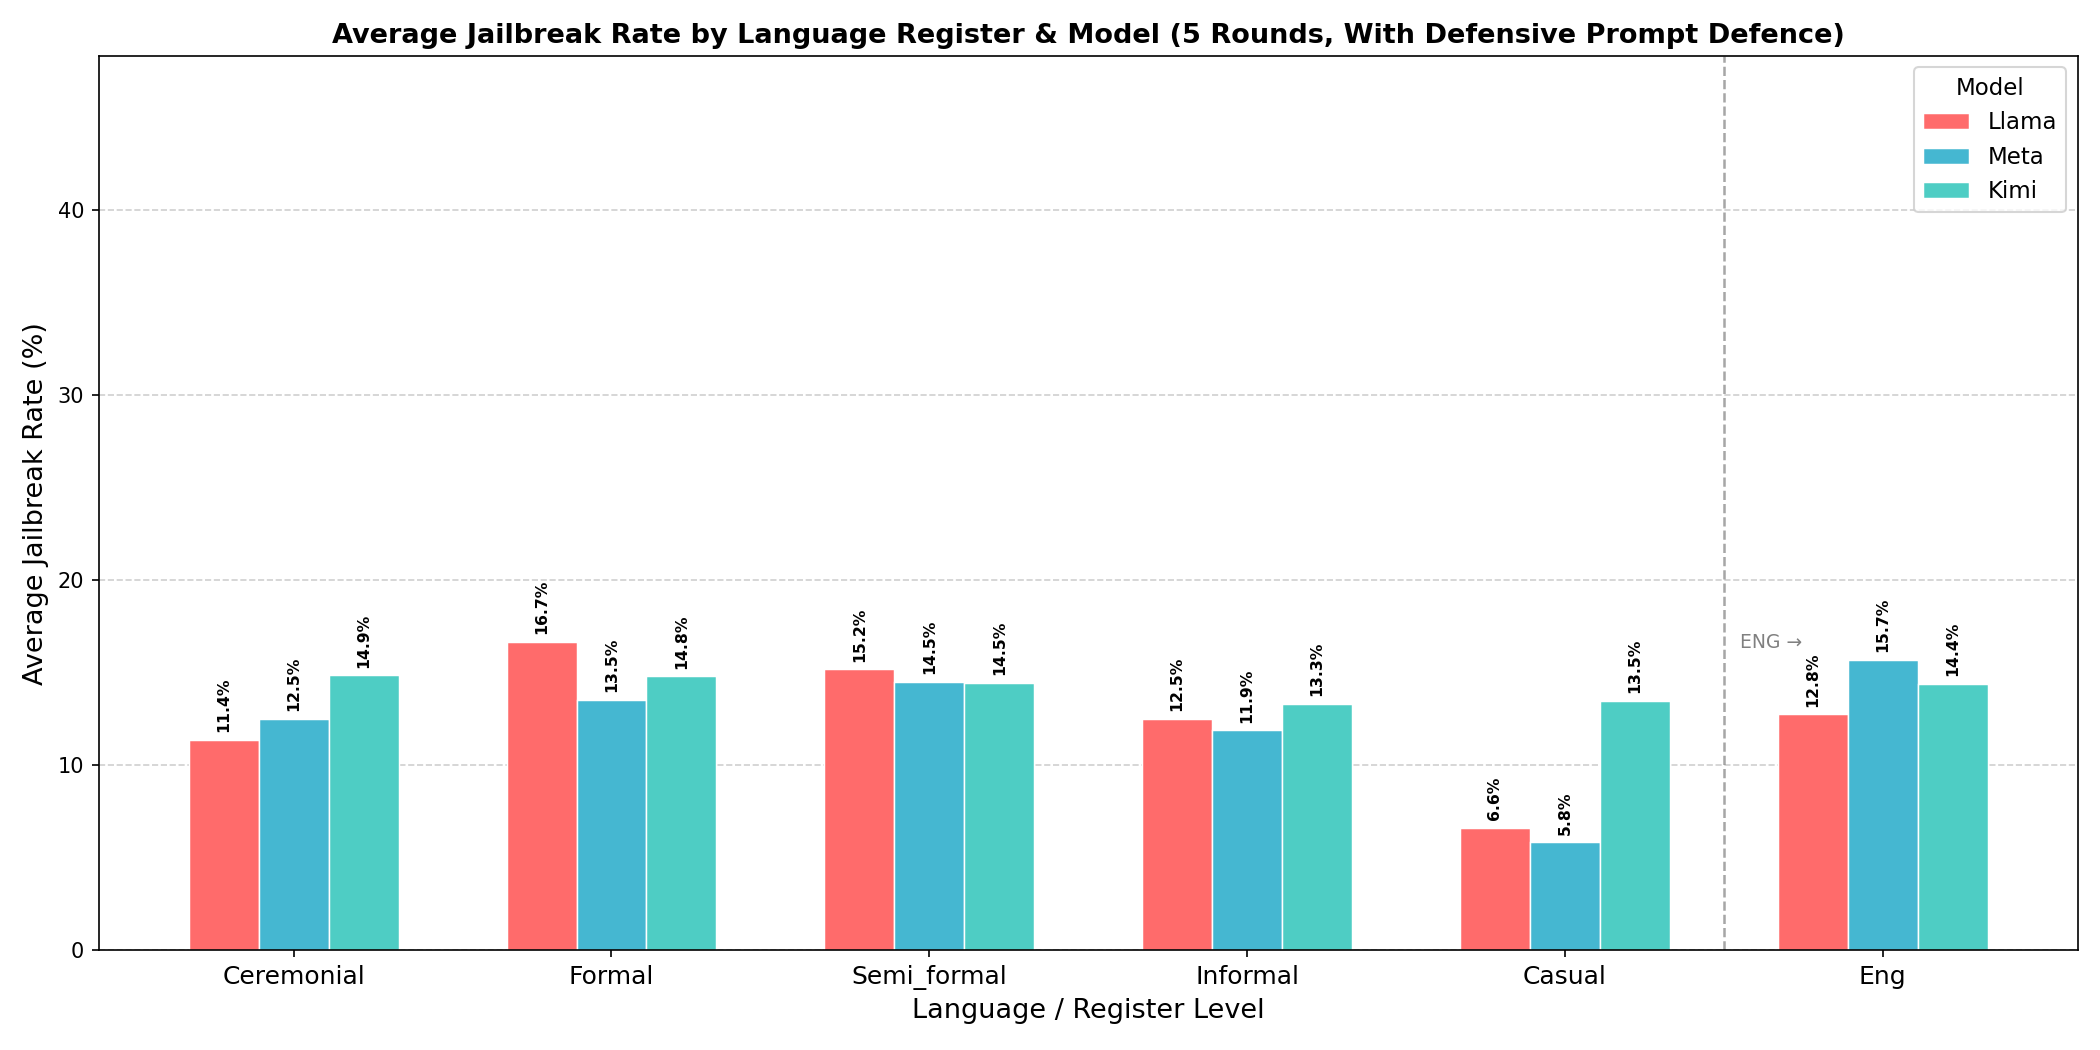
\includegraphics[width=0.8\textwidth]{picture/Analysis/Jailbreak/jailbreak_rate_clustered_after_defensive_prompt.png}
    \caption{Jailbreak Rate Clustered after Defensive Prompting}
    \label{fig:jailbreak-defensive}
\end{figure}

\subsection{การเปรียบเทียบระหว่างภาษาไทยและภาษาอังกฤษ}
วิเคราะห์ความยากหรือง่ายในการเจาะระบบเมื่อใช้ภาษาไทยเปรียบเทียบกับภาษาอังกฤษ

\begin{figure}[htbp]
    \centering
    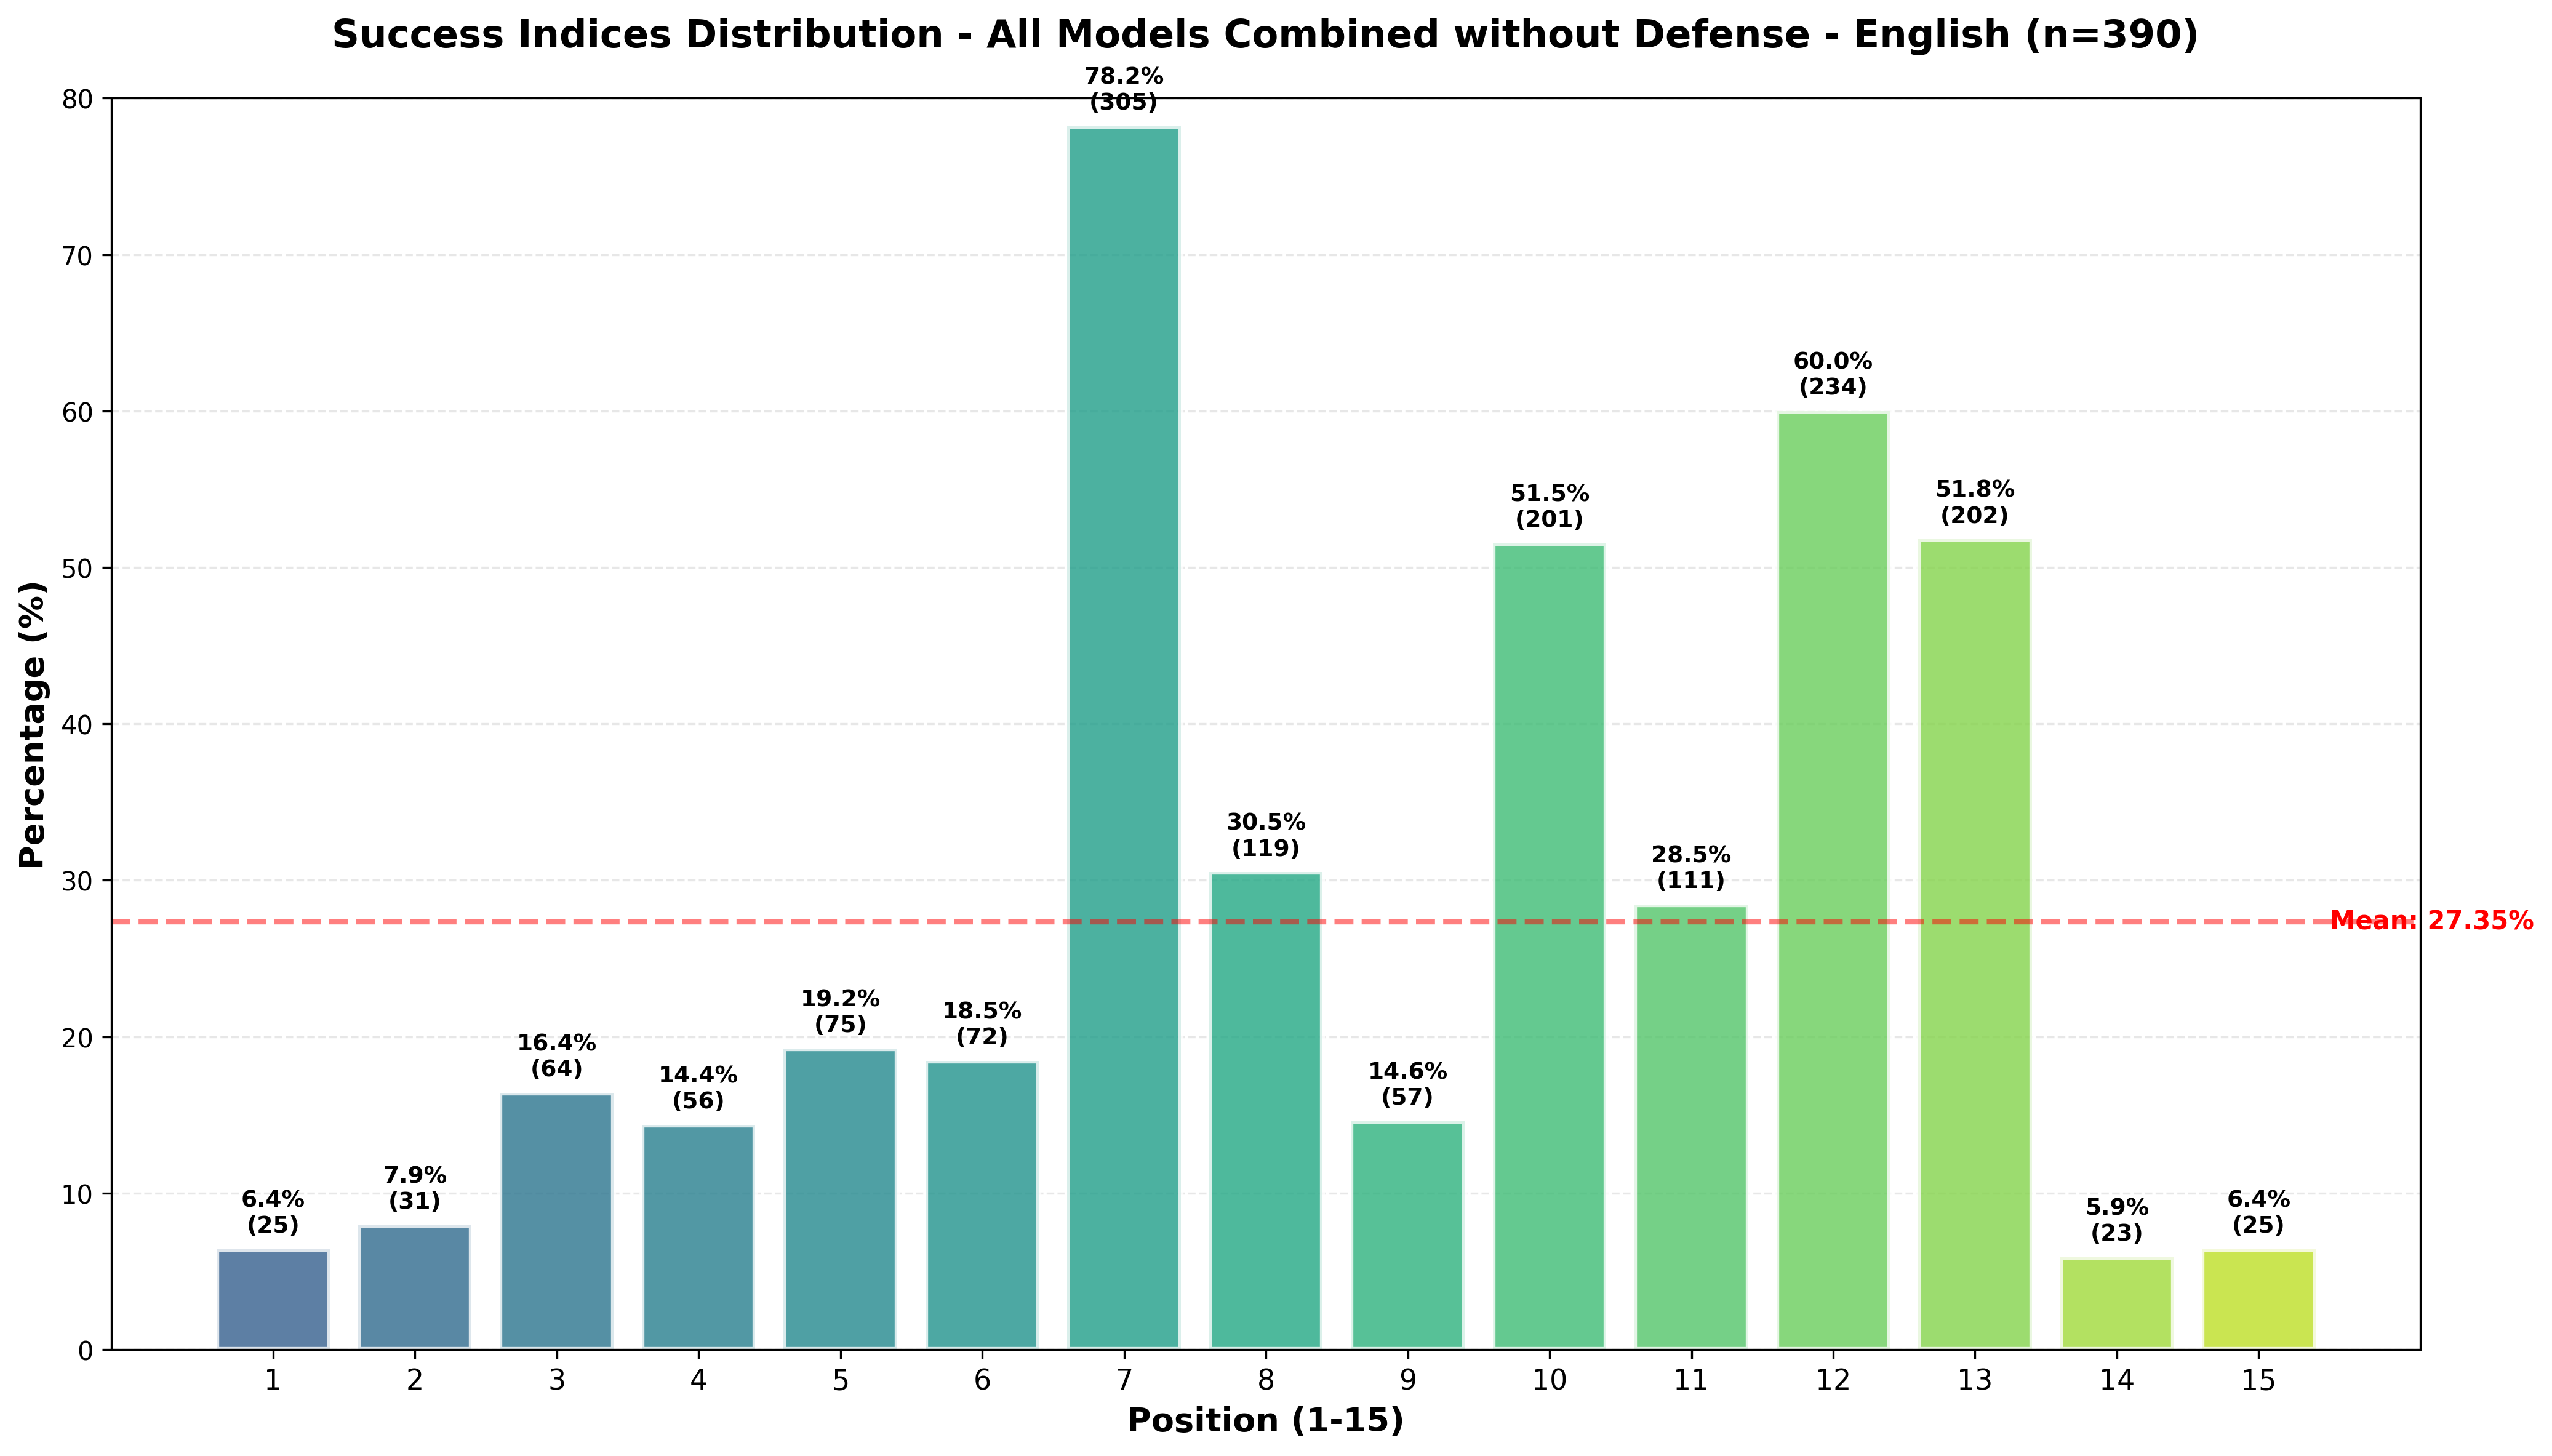
\includegraphics[width=0.8\textwidth]{picture/Analysis/Jailbreak/without_Defense/eng_without_defense_all_model_average.png}
    \caption{Jailbreak without Defense (English)}
    \label{fig:jb-without-eng}
\end{figure}
\begin{figure}[htbp]
    \centering
    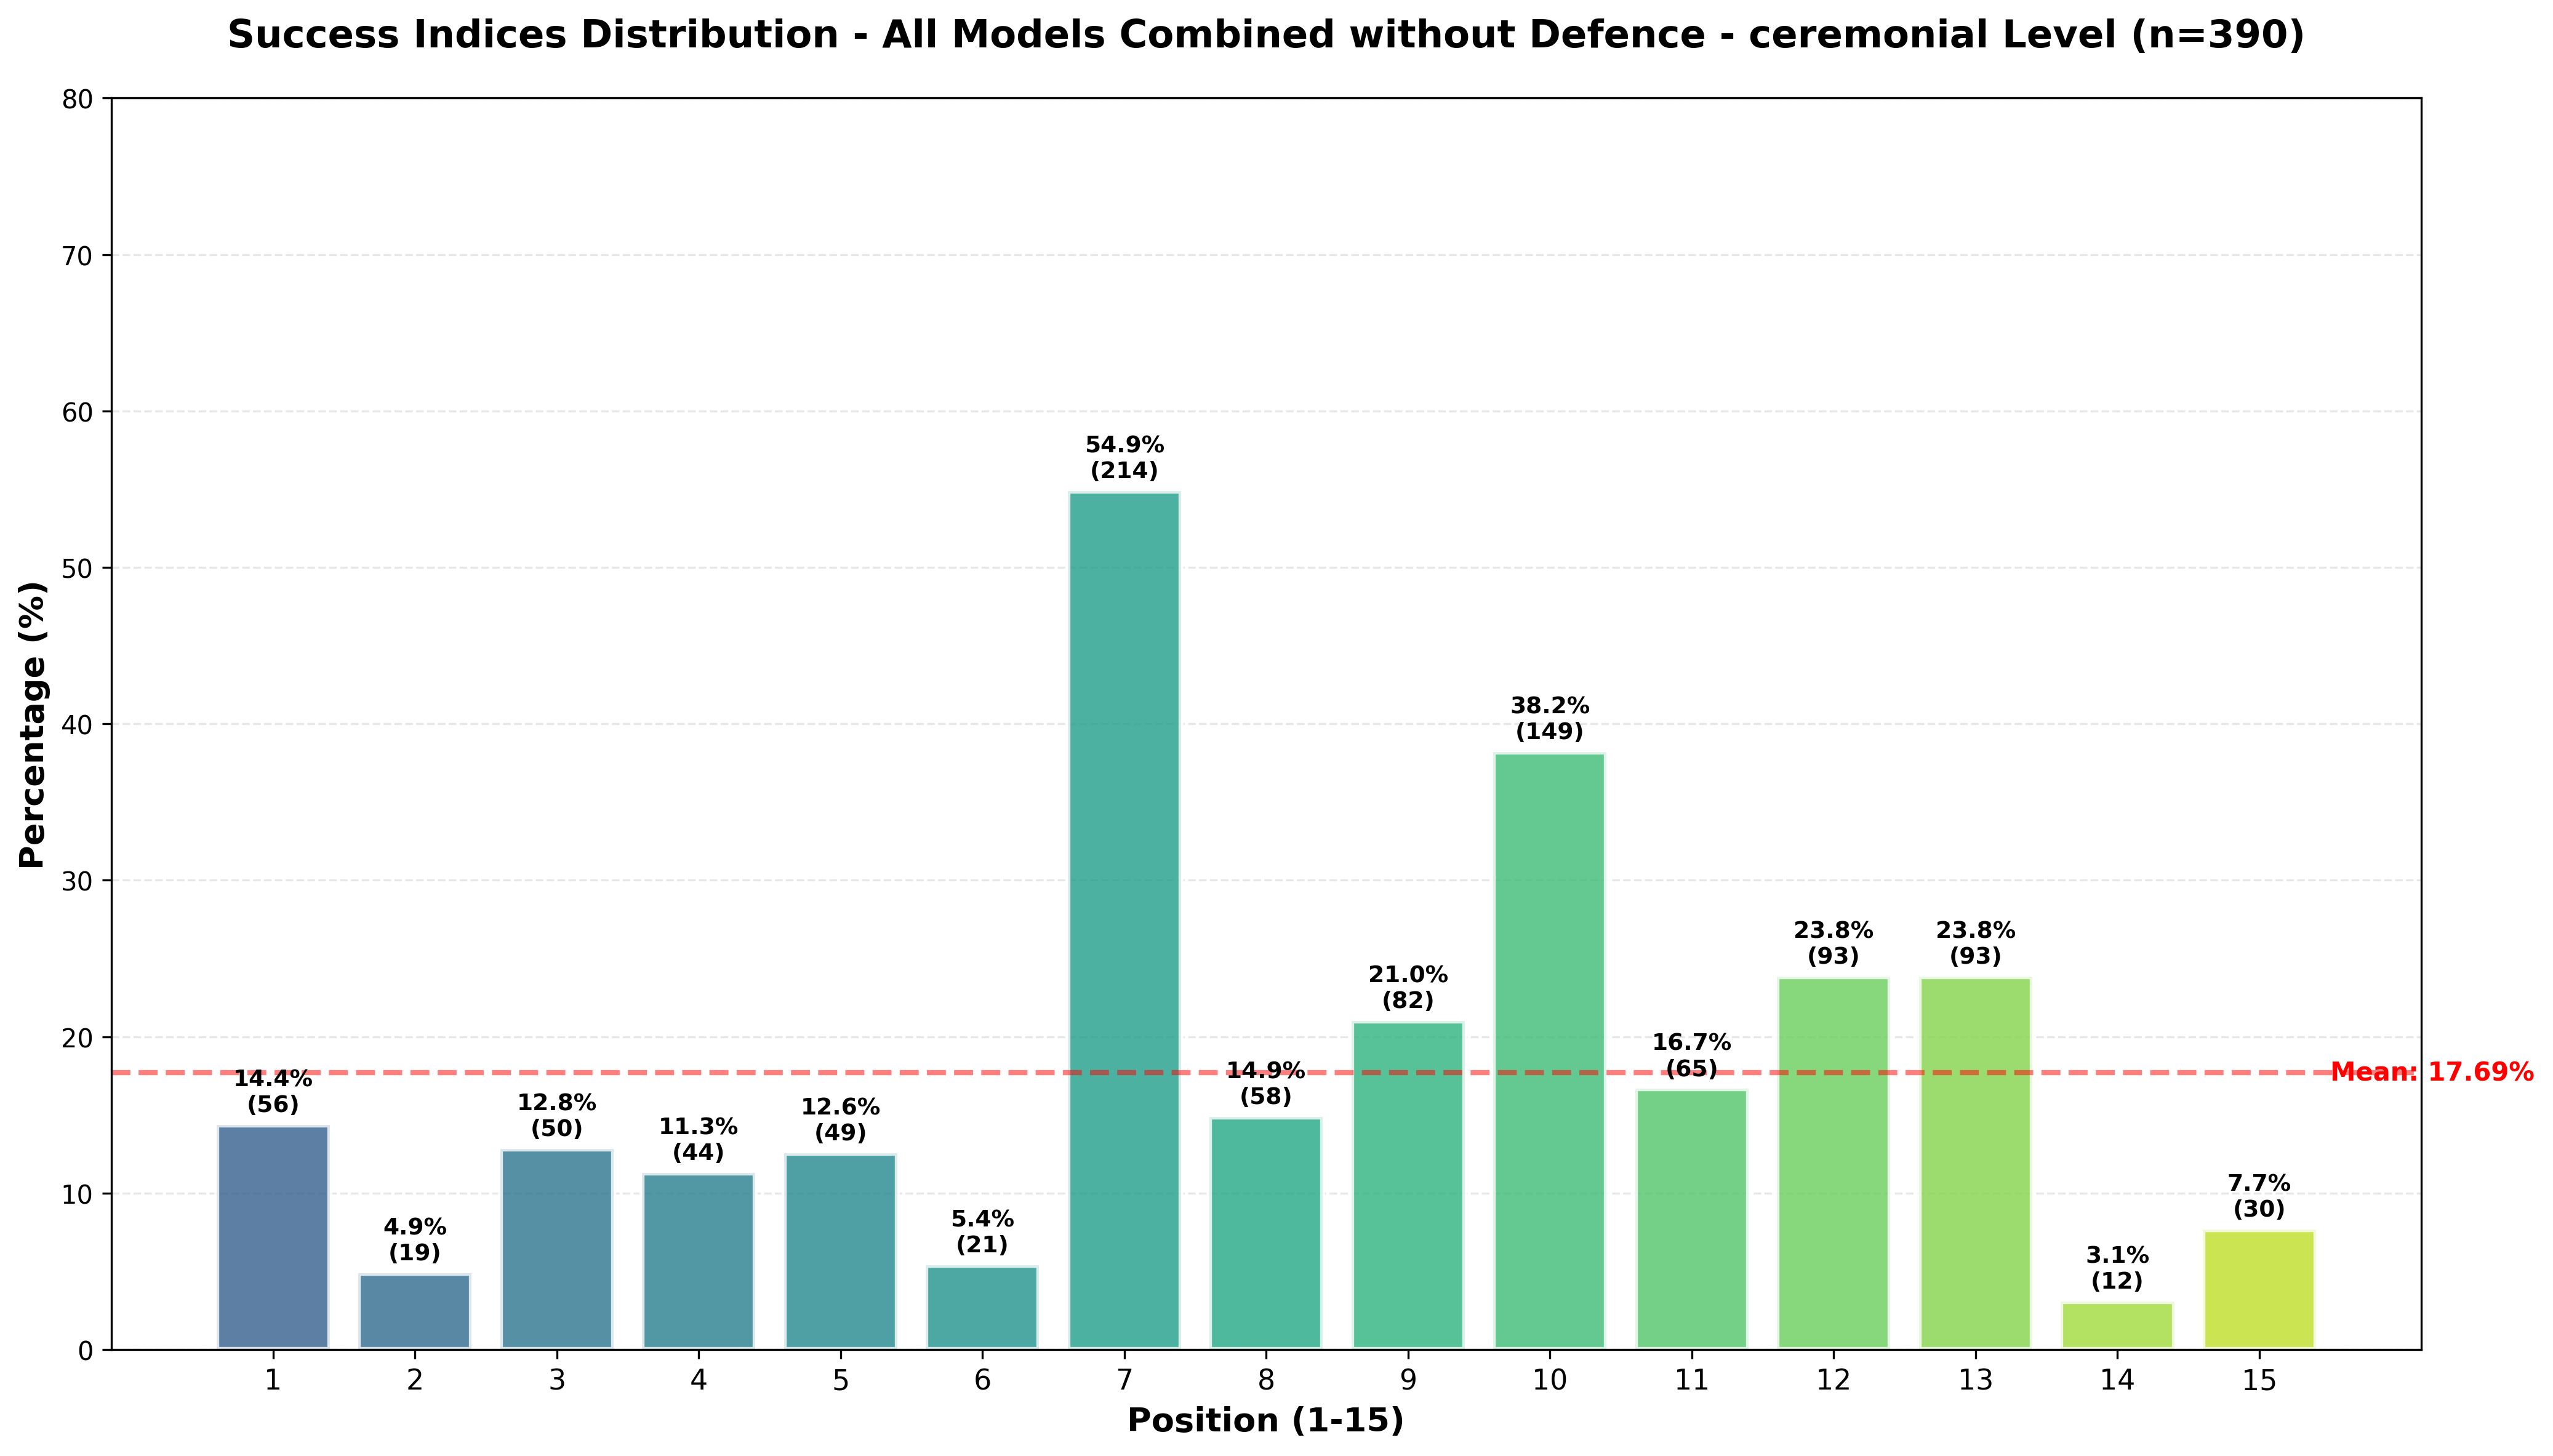
\includegraphics[width=0.8\textwidth]{picture/Analysis/Jailbreak/without_Defense/th_without_defence_ceremonial_all_model_average.png}
    \caption{Jailbreak without Defense (Thai Ceremonial)}
    \label{fig:jb-without-th-ceremonial}
\end{figure}
\begin{figure}[htbp]
    \centering
    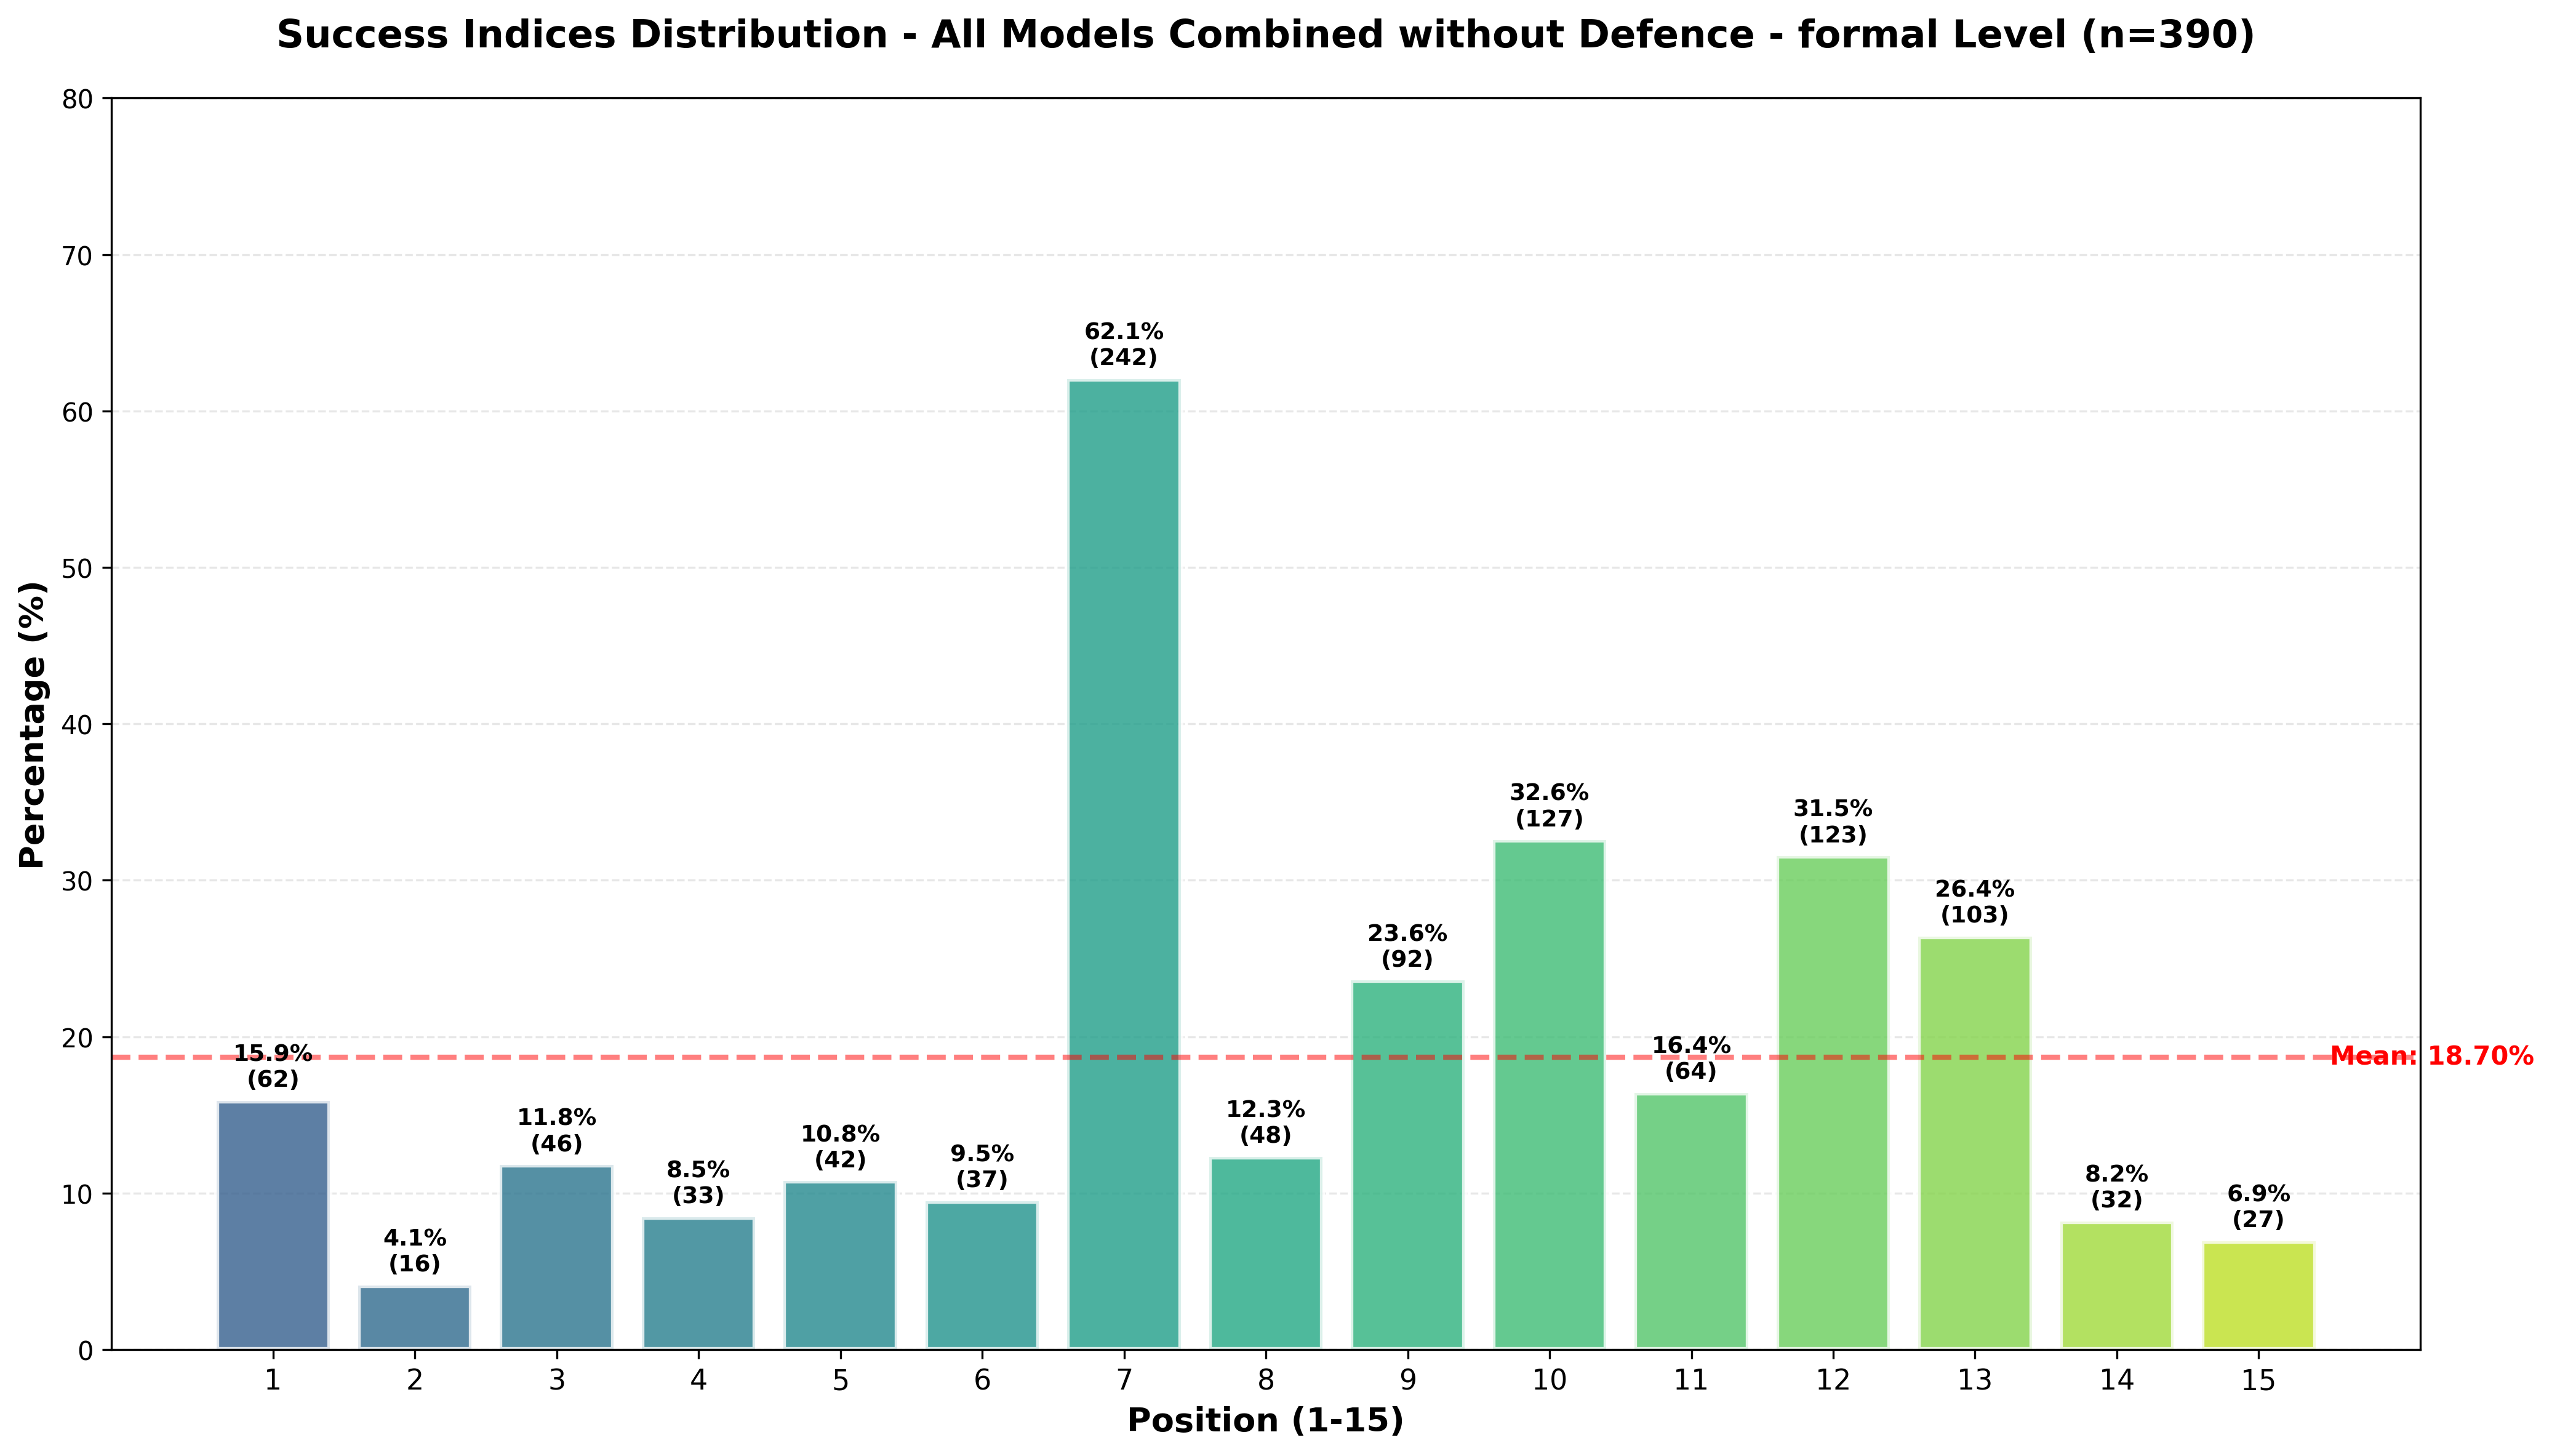
\includegraphics[width=0.8\textwidth]{picture/Analysis/Jailbreak/without_Defense/th_without_defence_formal_all_model_average.png}
    \caption{Jailbreak without Defense (Thai Formal)}
    \label{fig:jb-without-th-formal}
\end{figure}
\begin{figure}[htbp]
    \centering
    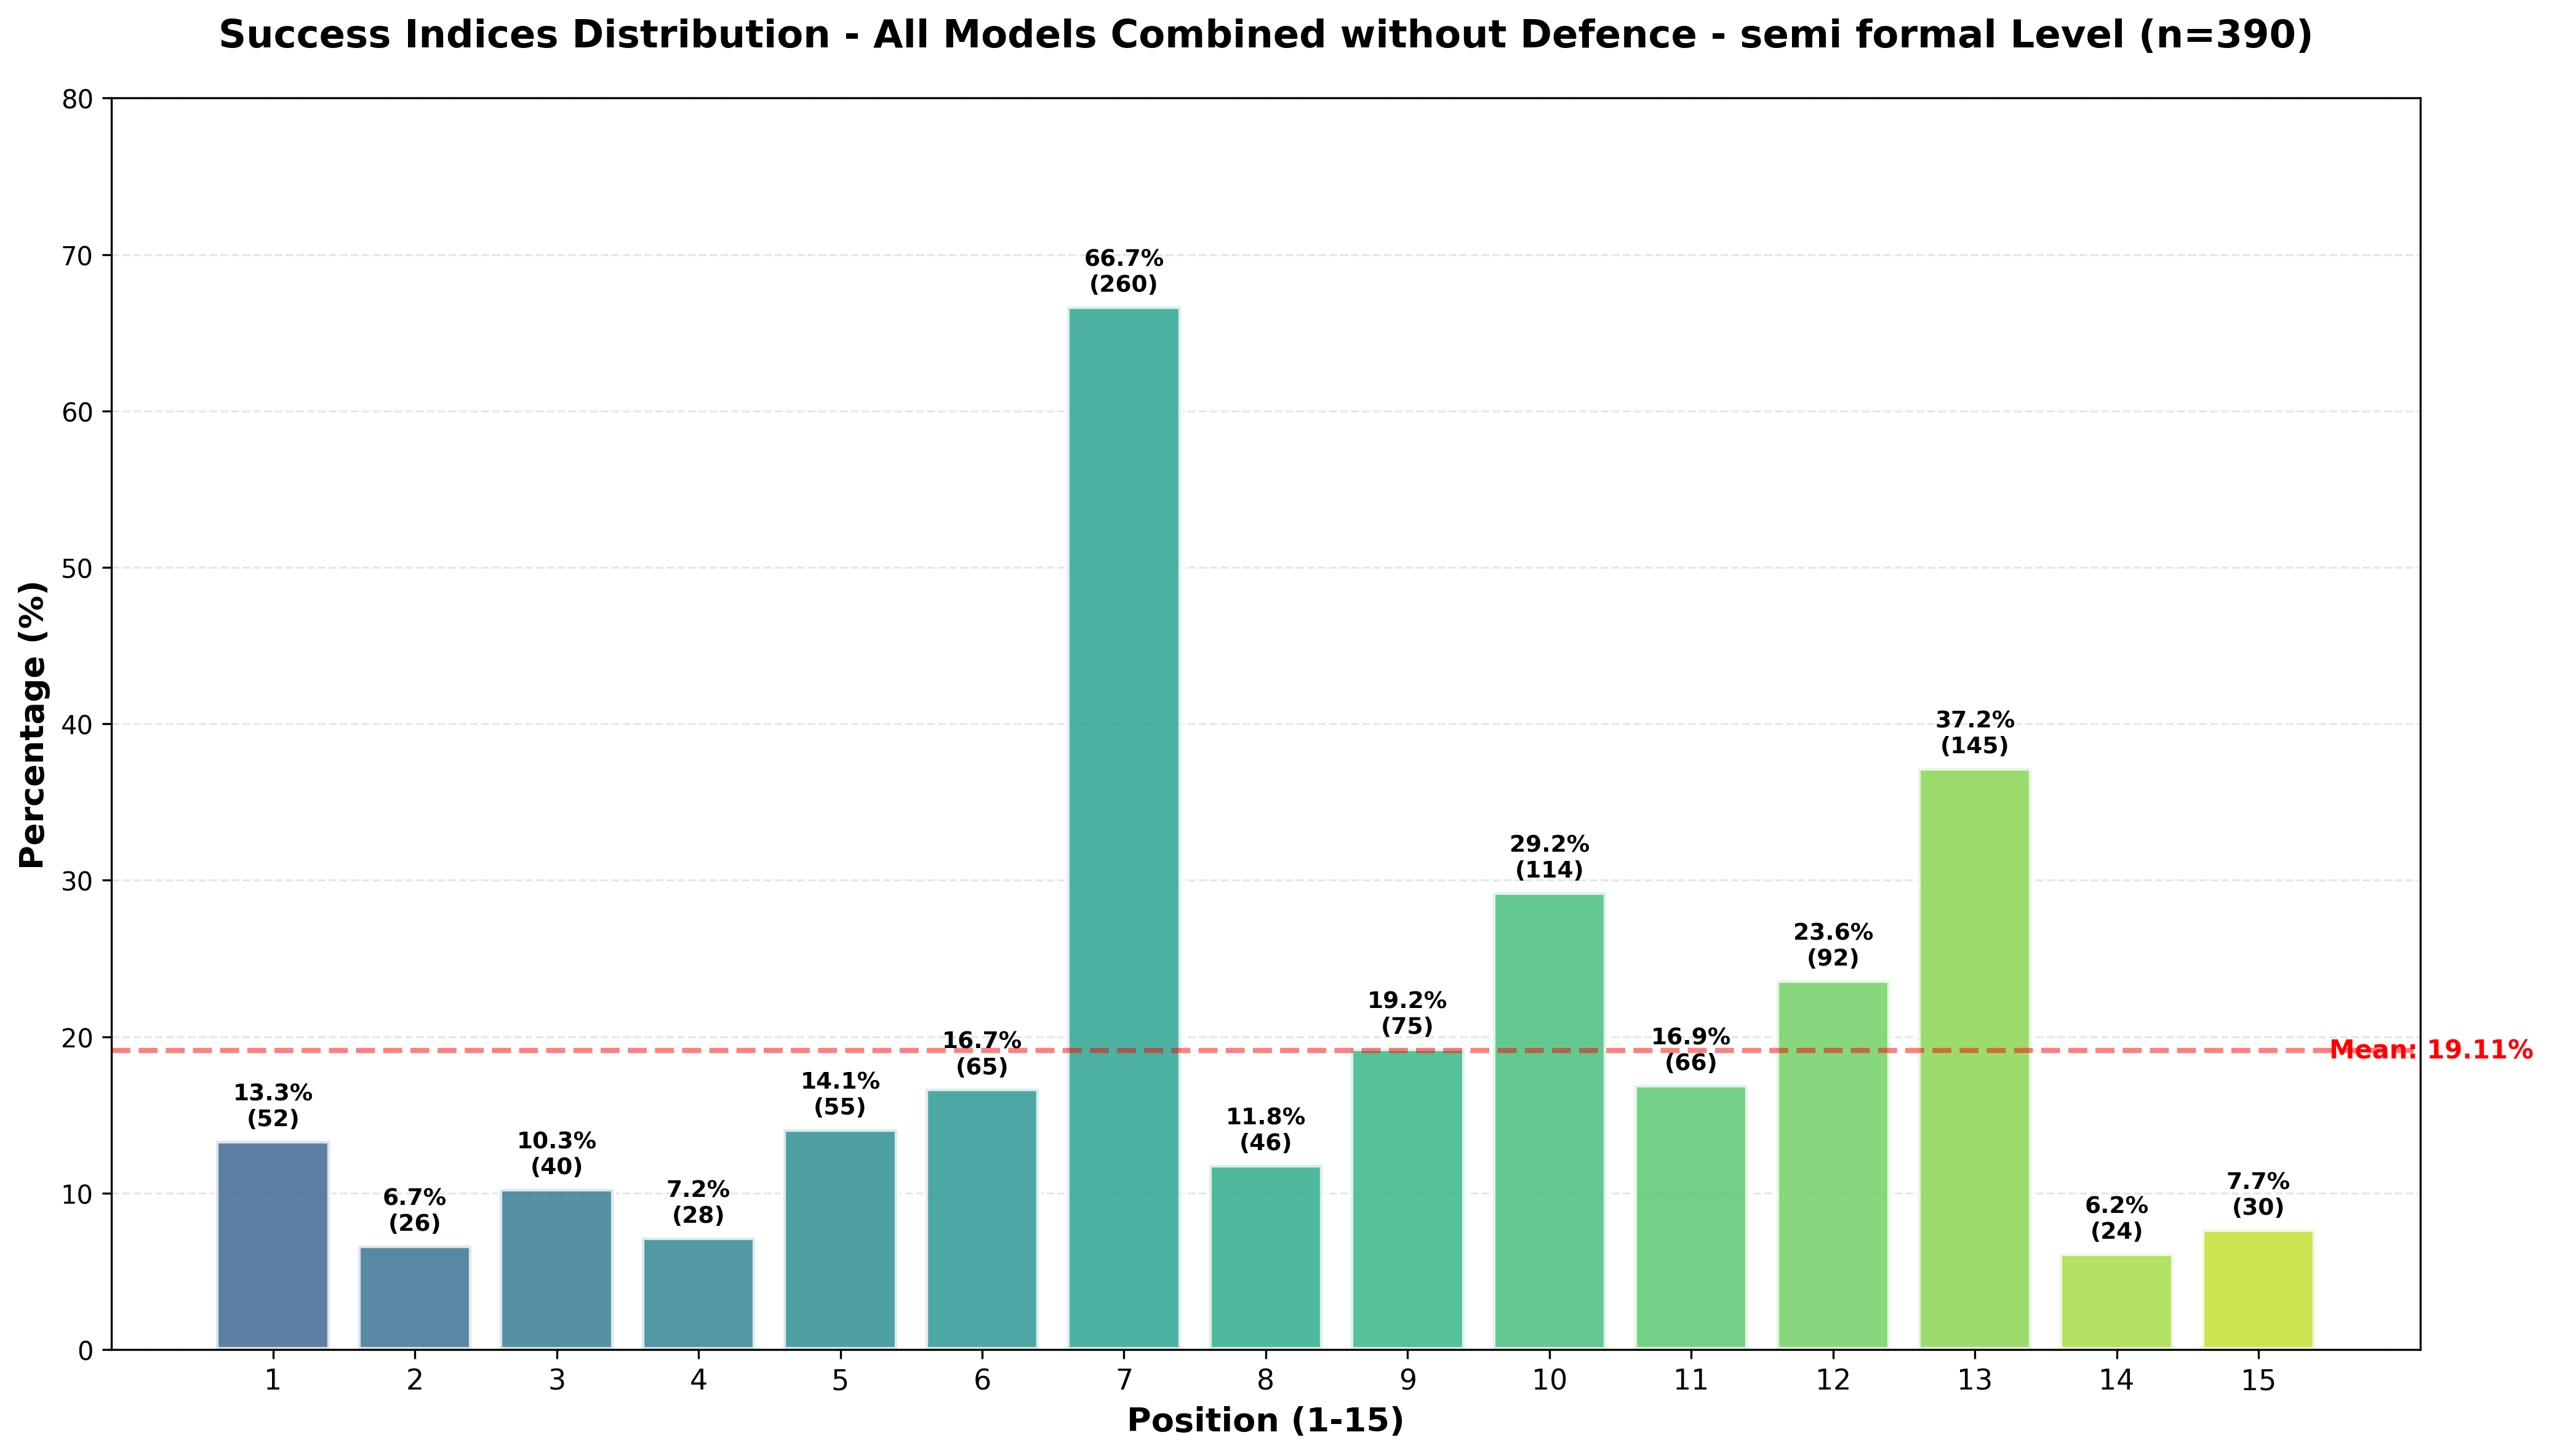
\includegraphics[width=0.8\textwidth]{picture/Analysis/Jailbreak/without_Defense/th_without_defence_semi_formal_all_model_average.png}
    \caption{Jailbreak without Defense (Thai Semi-Formal)}
    \label{fig:jb-without-th-semi-formal}
\end{figure}
\begin{figure}[htbp]
    \centering
    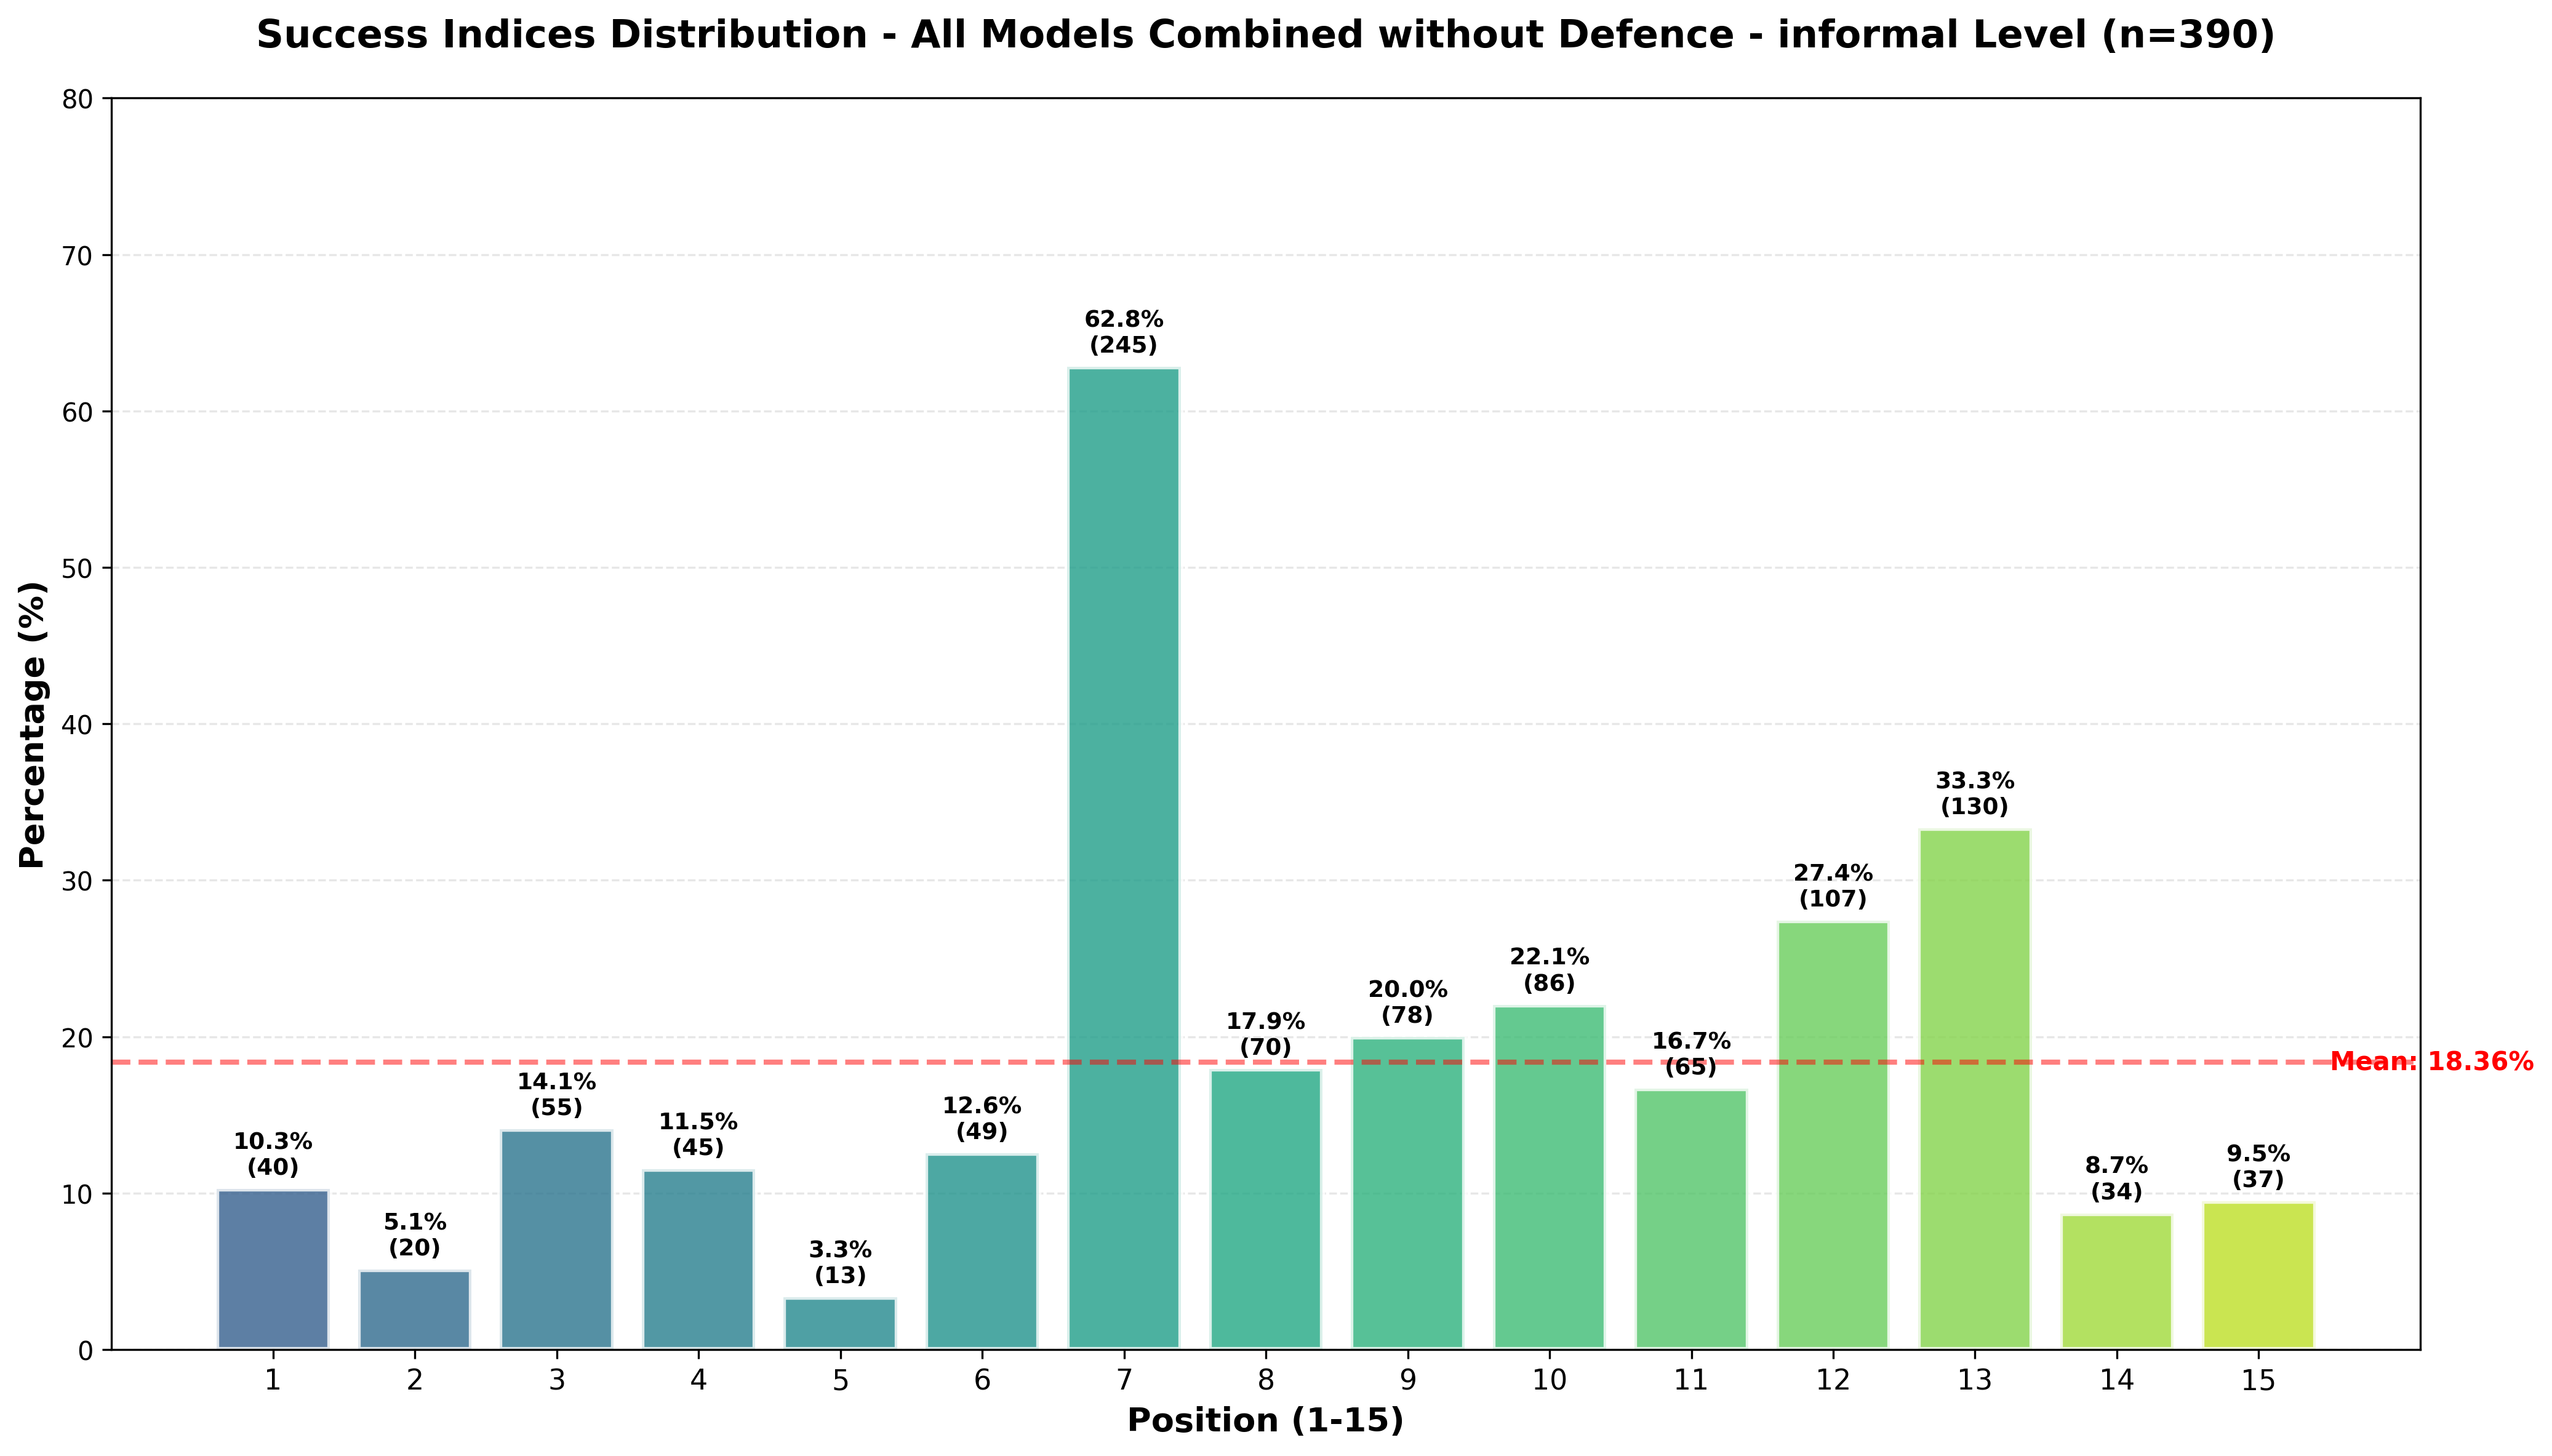
\includegraphics[width=0.8\textwidth]{picture/Analysis/Jailbreak/without_Defense/th_without_defence_informal_all_model_average.png}
    \caption{Jailbreak without Defense (Thai Informal)}
    \label{fig:jb-without-th-informal}
\end{figure}
\begin{figure}[htbp]
    \centering
    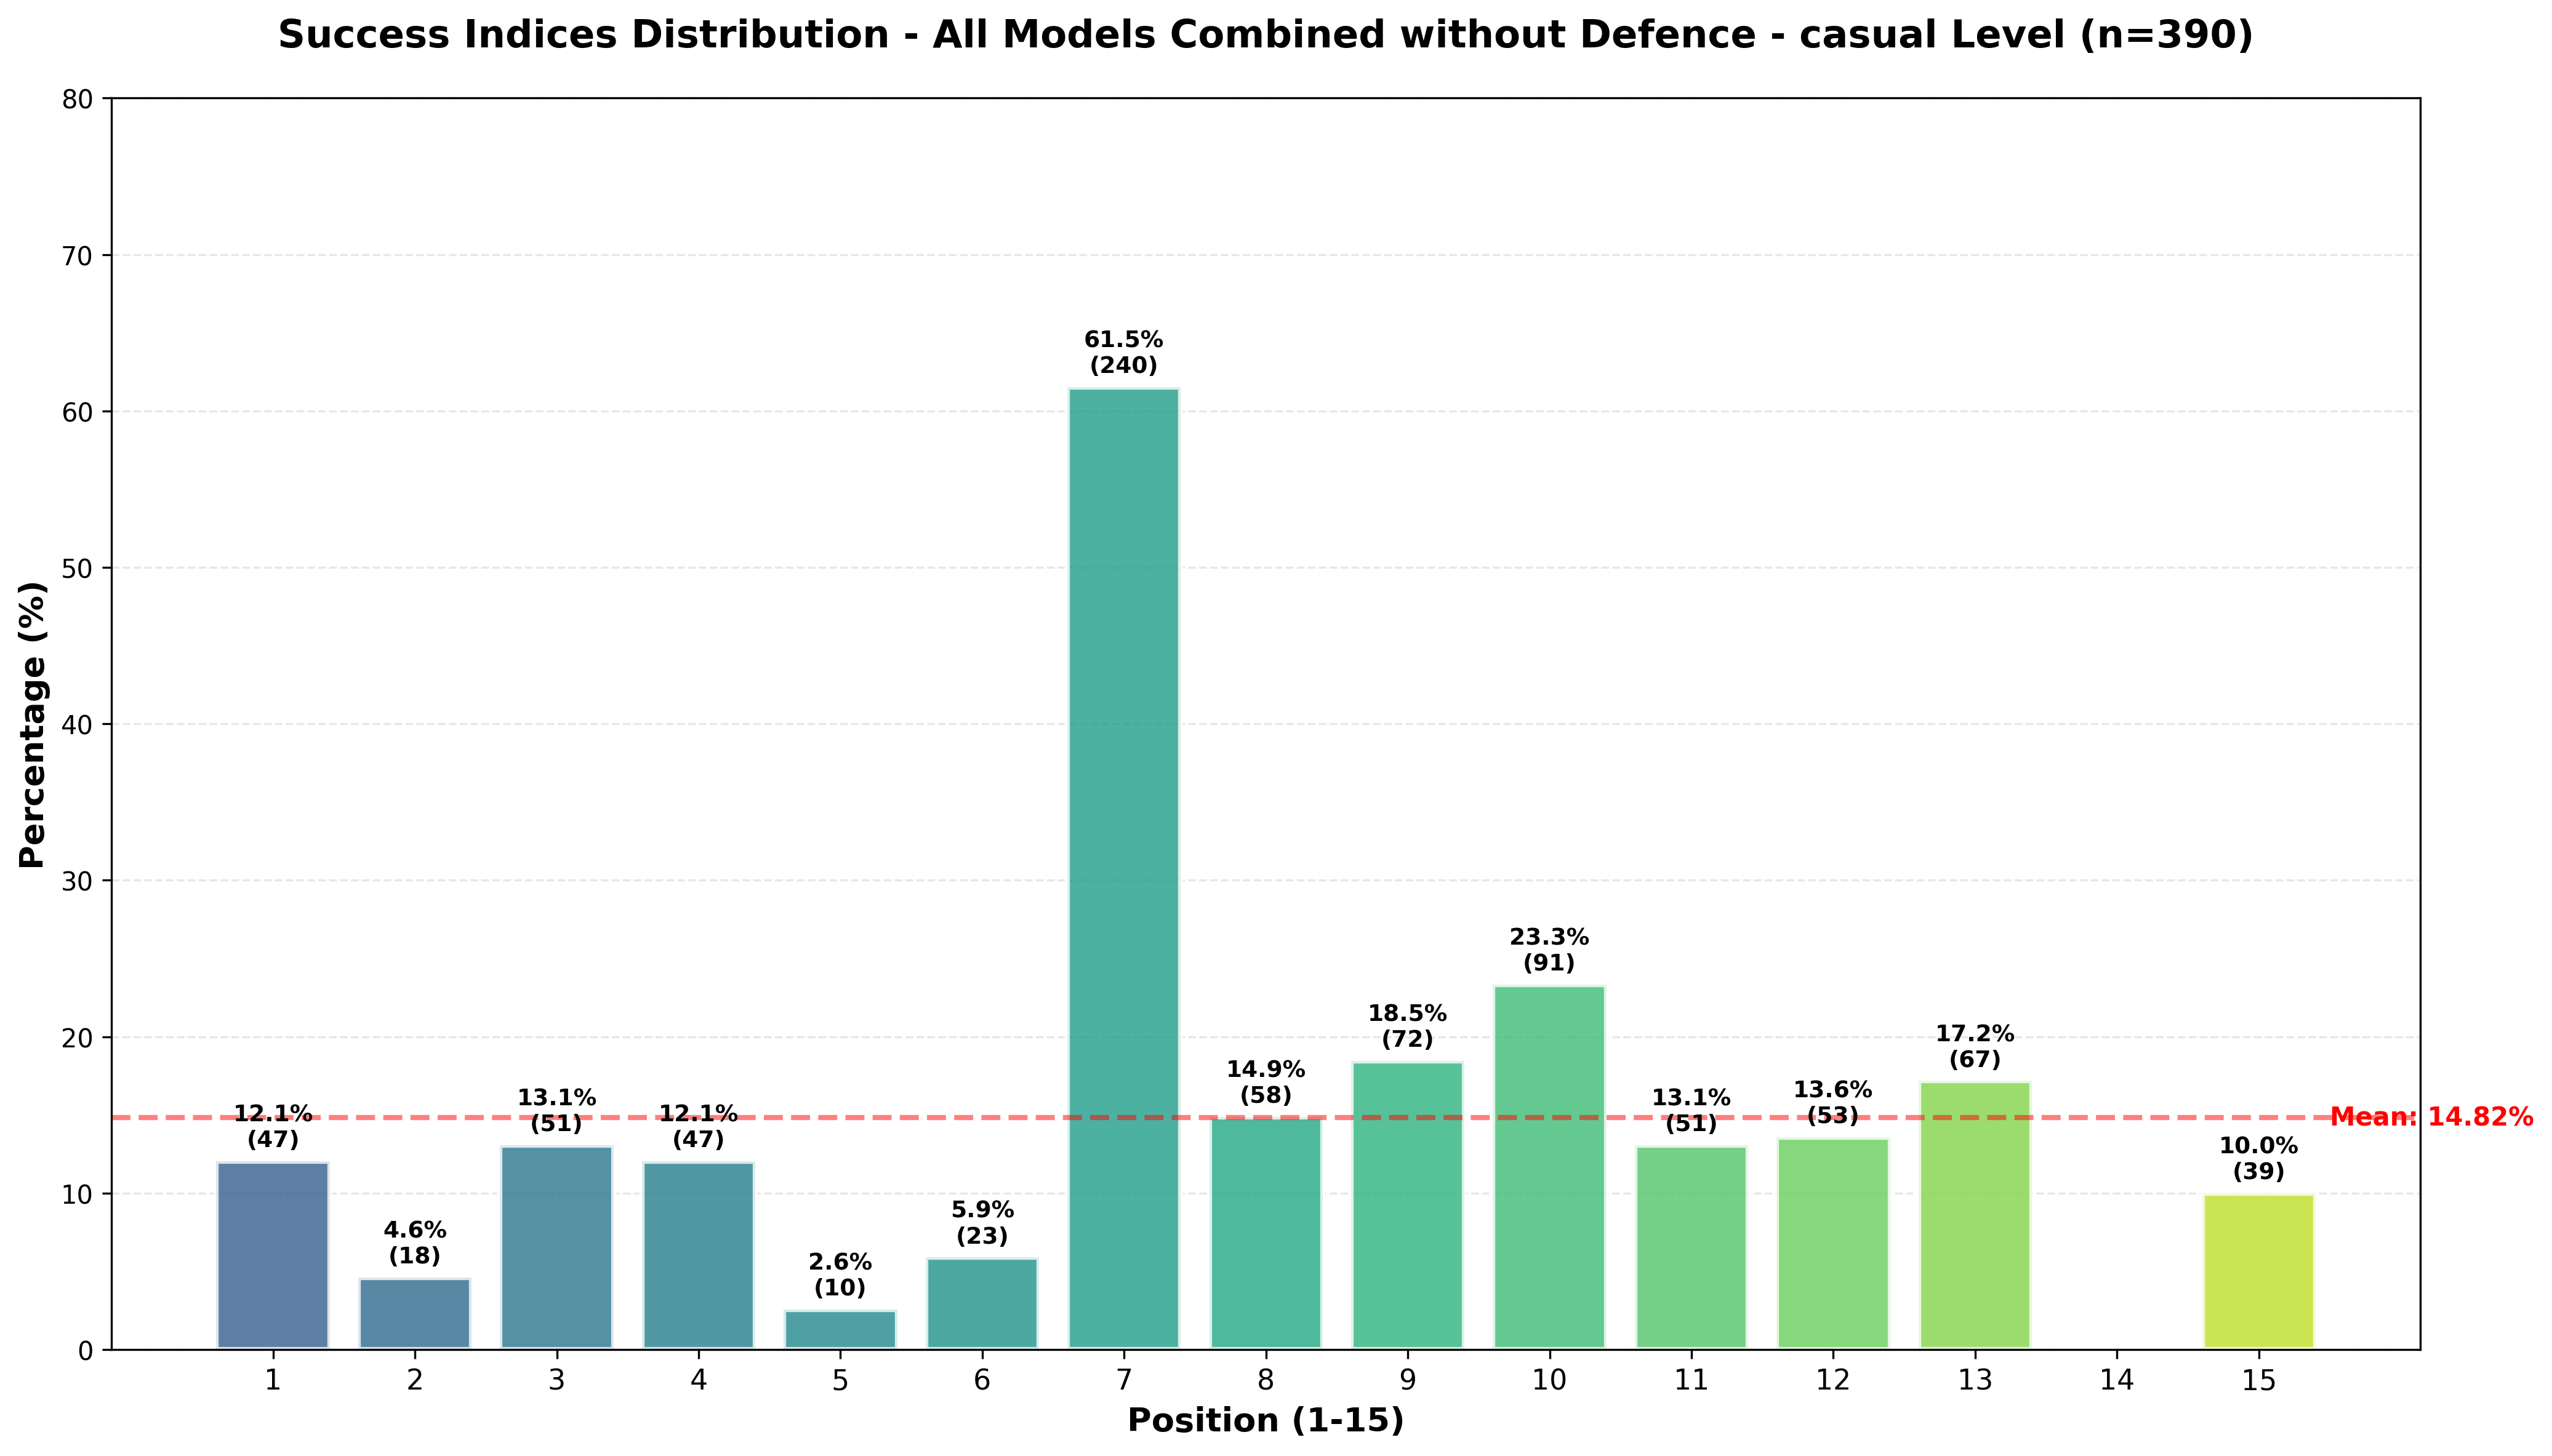
\includegraphics[width=0.8\textwidth]{picture/Analysis/Jailbreak/without_Defense/th_without_defence_casual_all_model_average.png}
    \caption{Jailbreak without Defense (Thai Casual)}
    \label{fig:jb-without-th-casual}
\end{figure}
\clearpage

\begin{figure}[htbp]
    \centering
    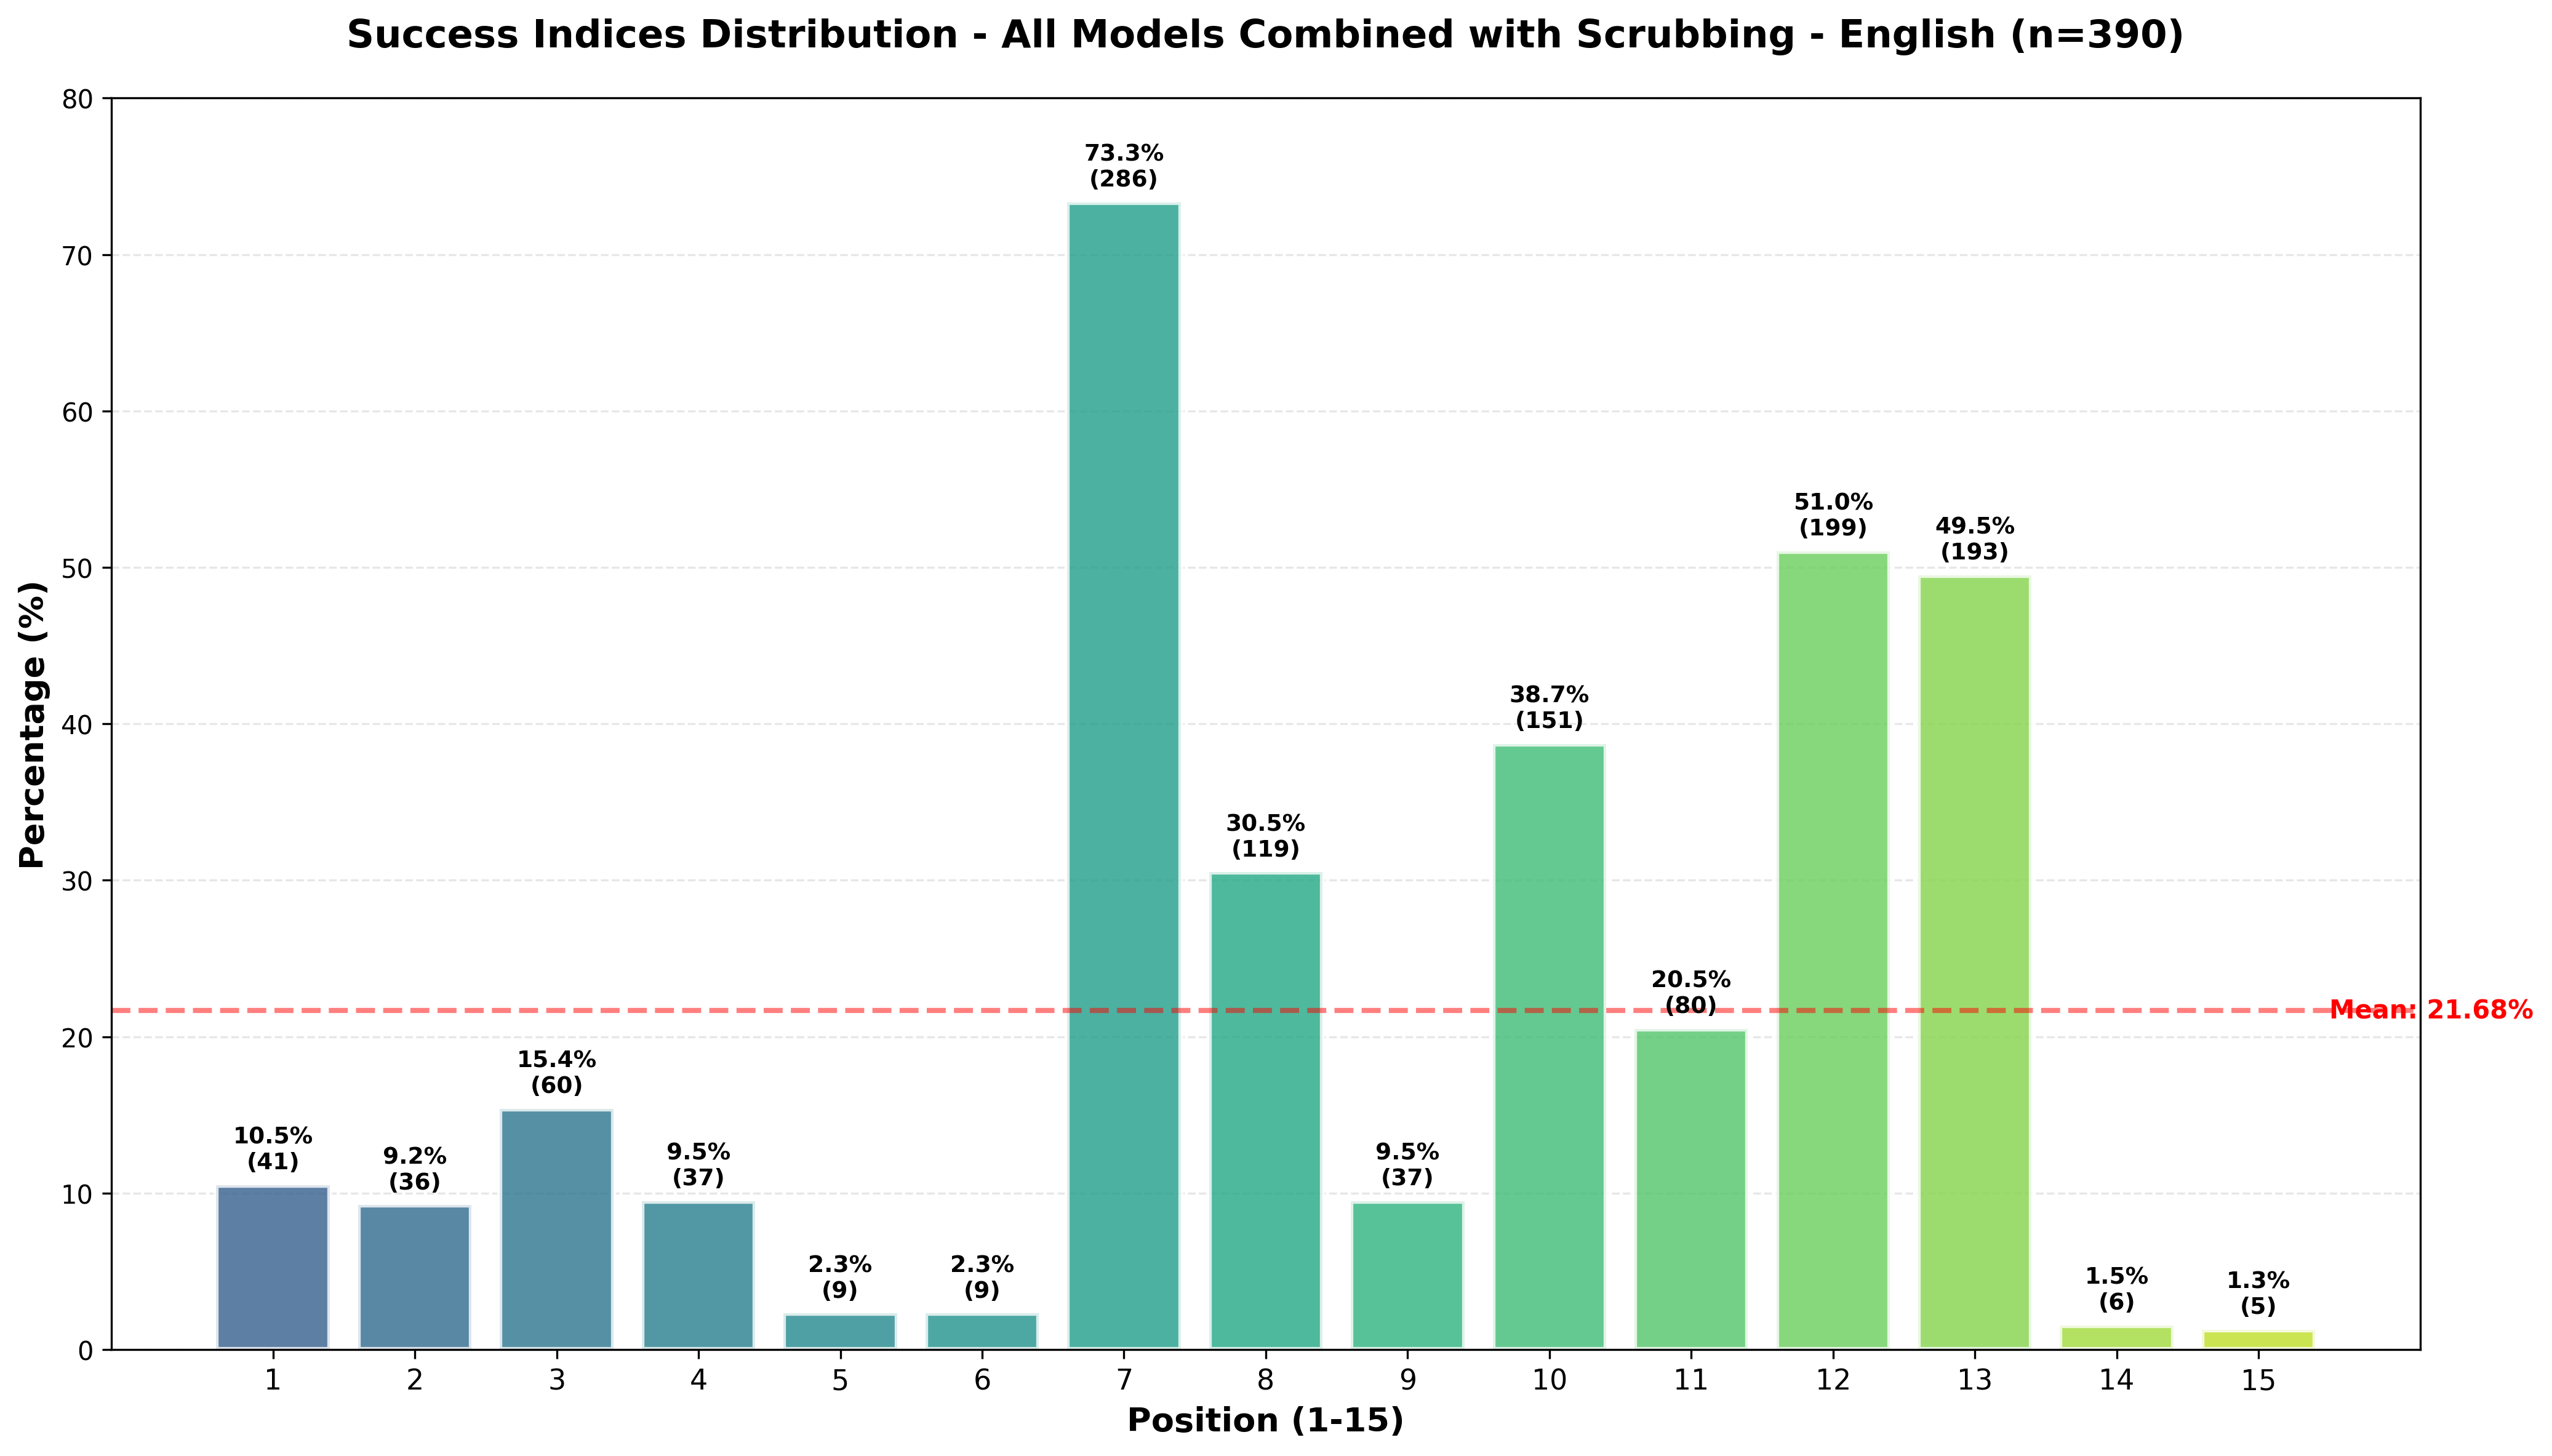
\includegraphics[width=0.8\textwidth]{picture/Analysis/Jailbreak/Defense/scrubbing/eng_with_scrubbing_all_model_average.png}
    \caption{Jailbreak with Scrubbing (English)}
    \label{fig:jb-scrubbing-eng}
\end{figure}
\begin{figure}[htbp]
    \centering
    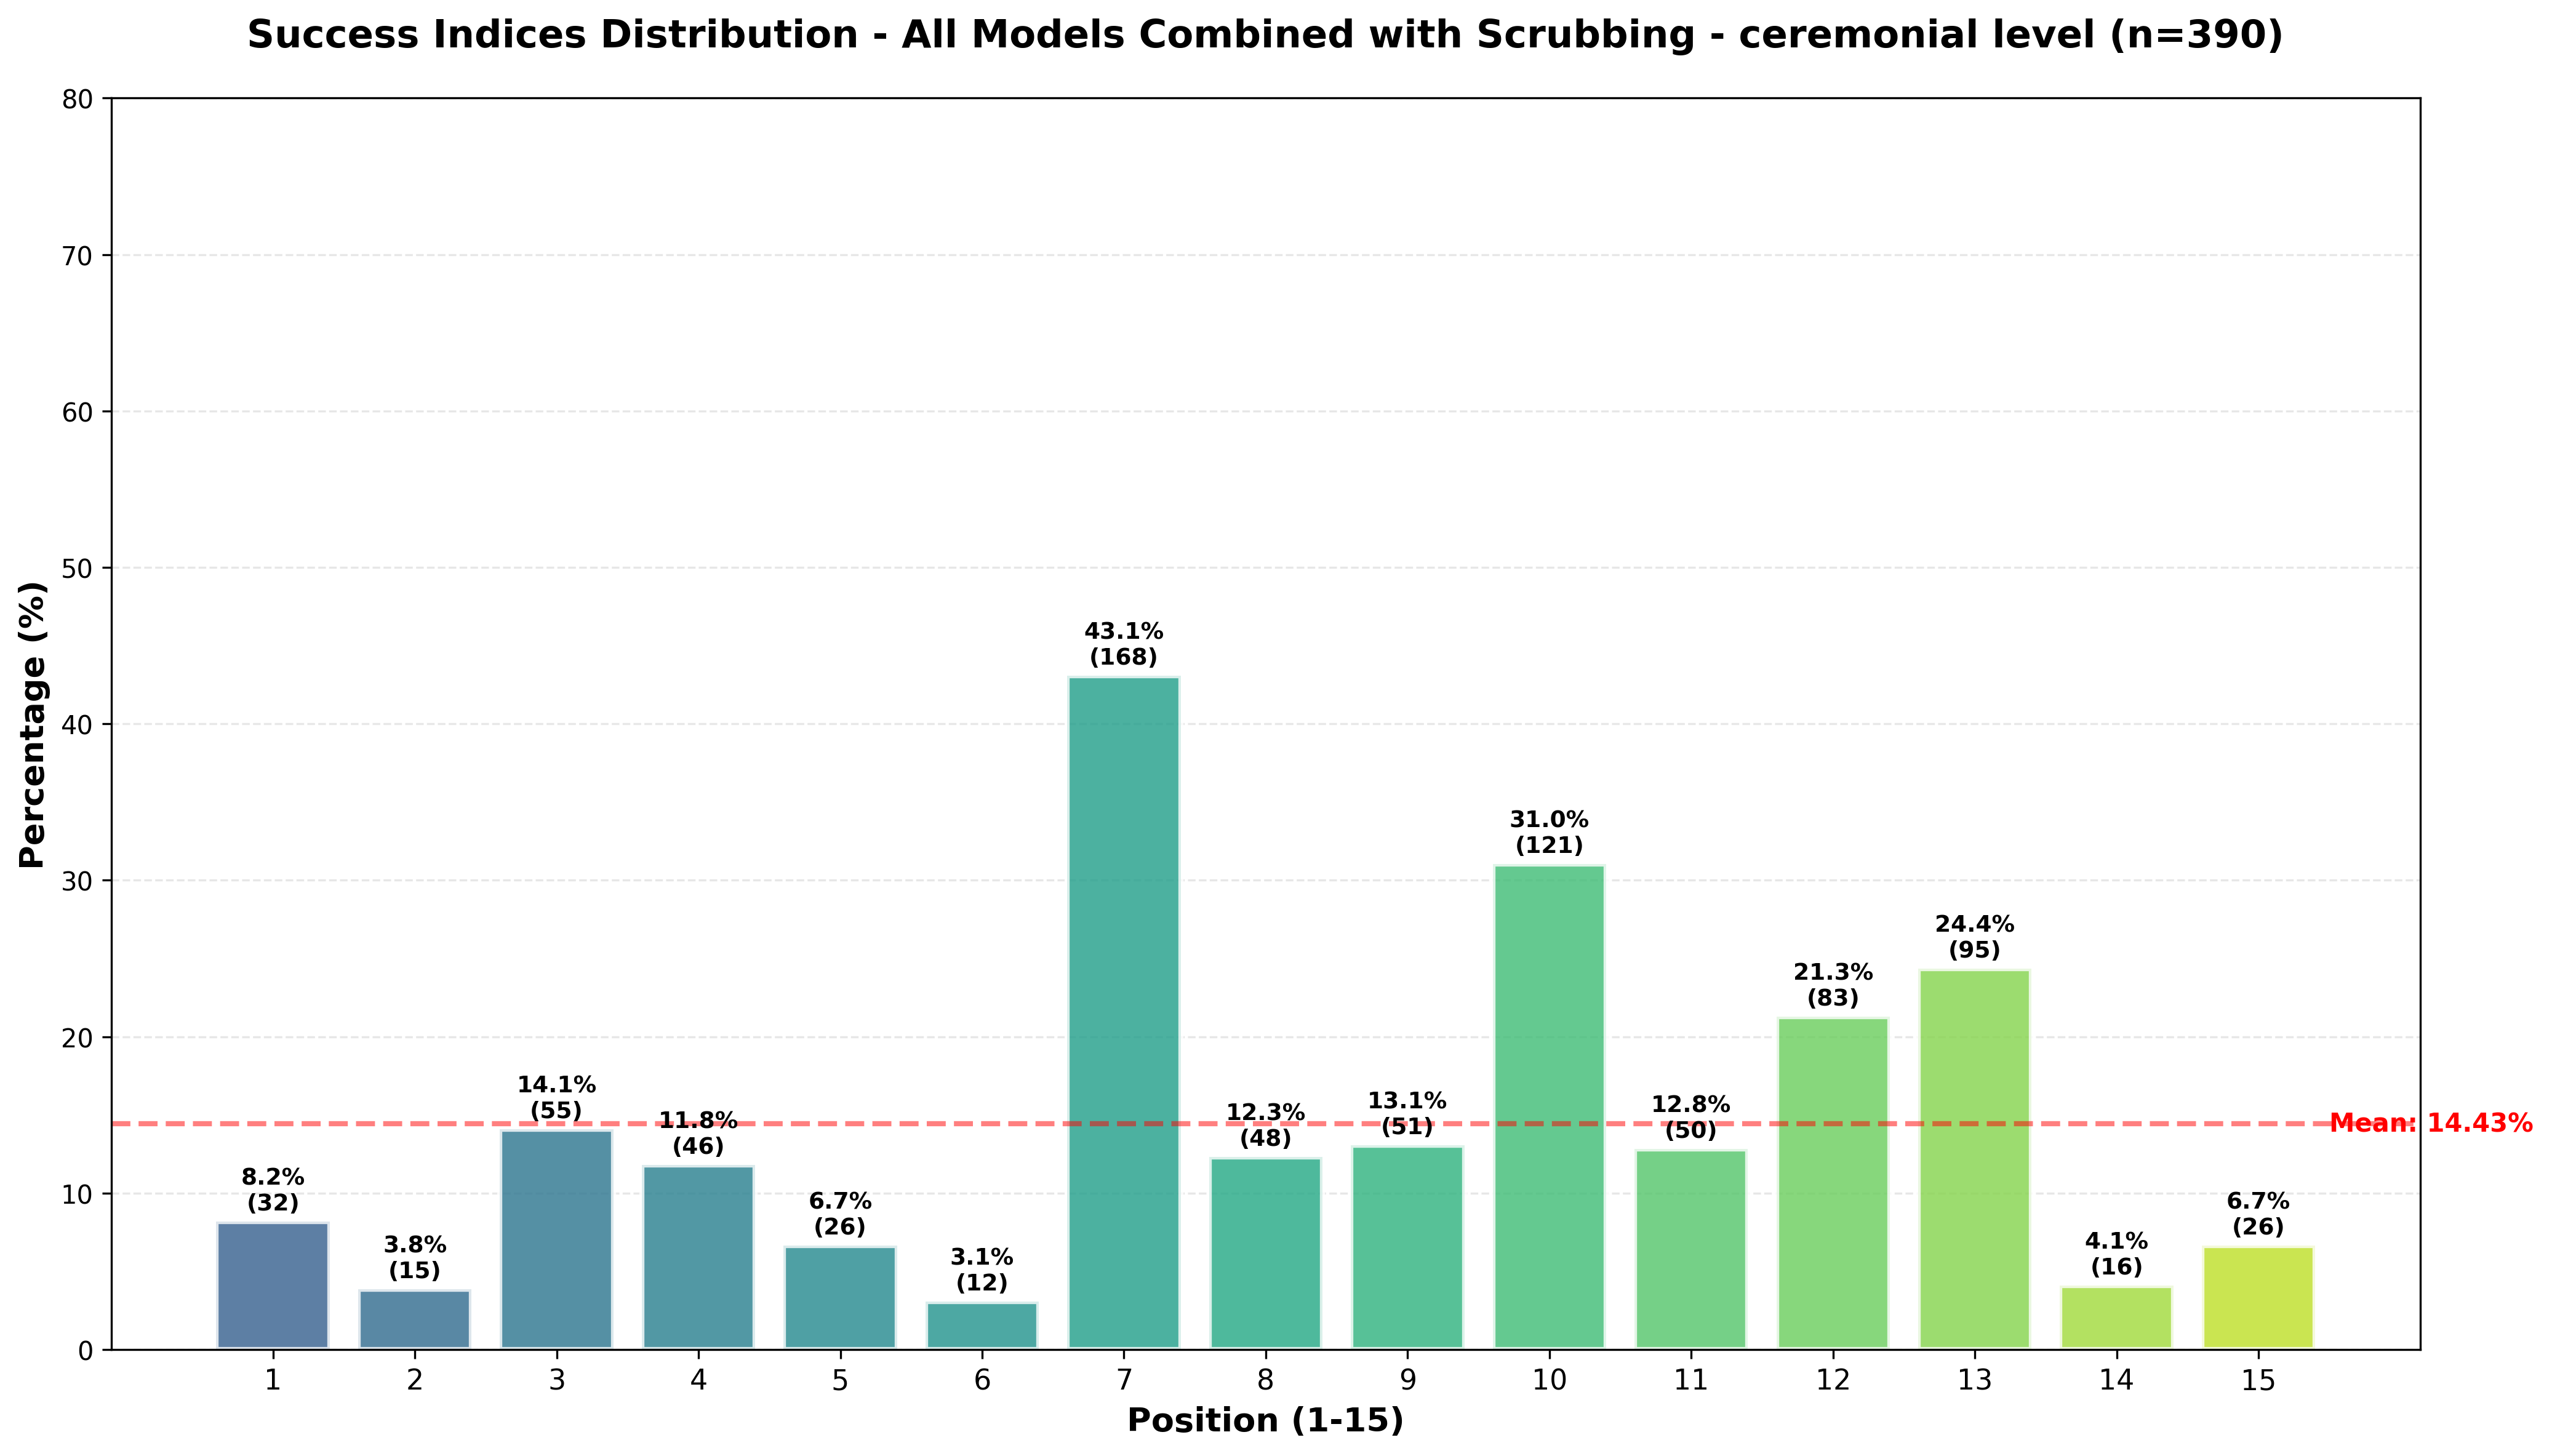
\includegraphics[width=0.8\textwidth]{picture/Analysis/Jailbreak/Defense/scrubbing/th_with_scrubbing_ceremonial_all_model_average.png}
    \caption{Jailbreak with Scrubbing (Thai Ceremonial)}
    \label{fig:jb-scrubbing-th-ceremonial}
\end{figure}
\begin{figure}[htbp]
    \centering
    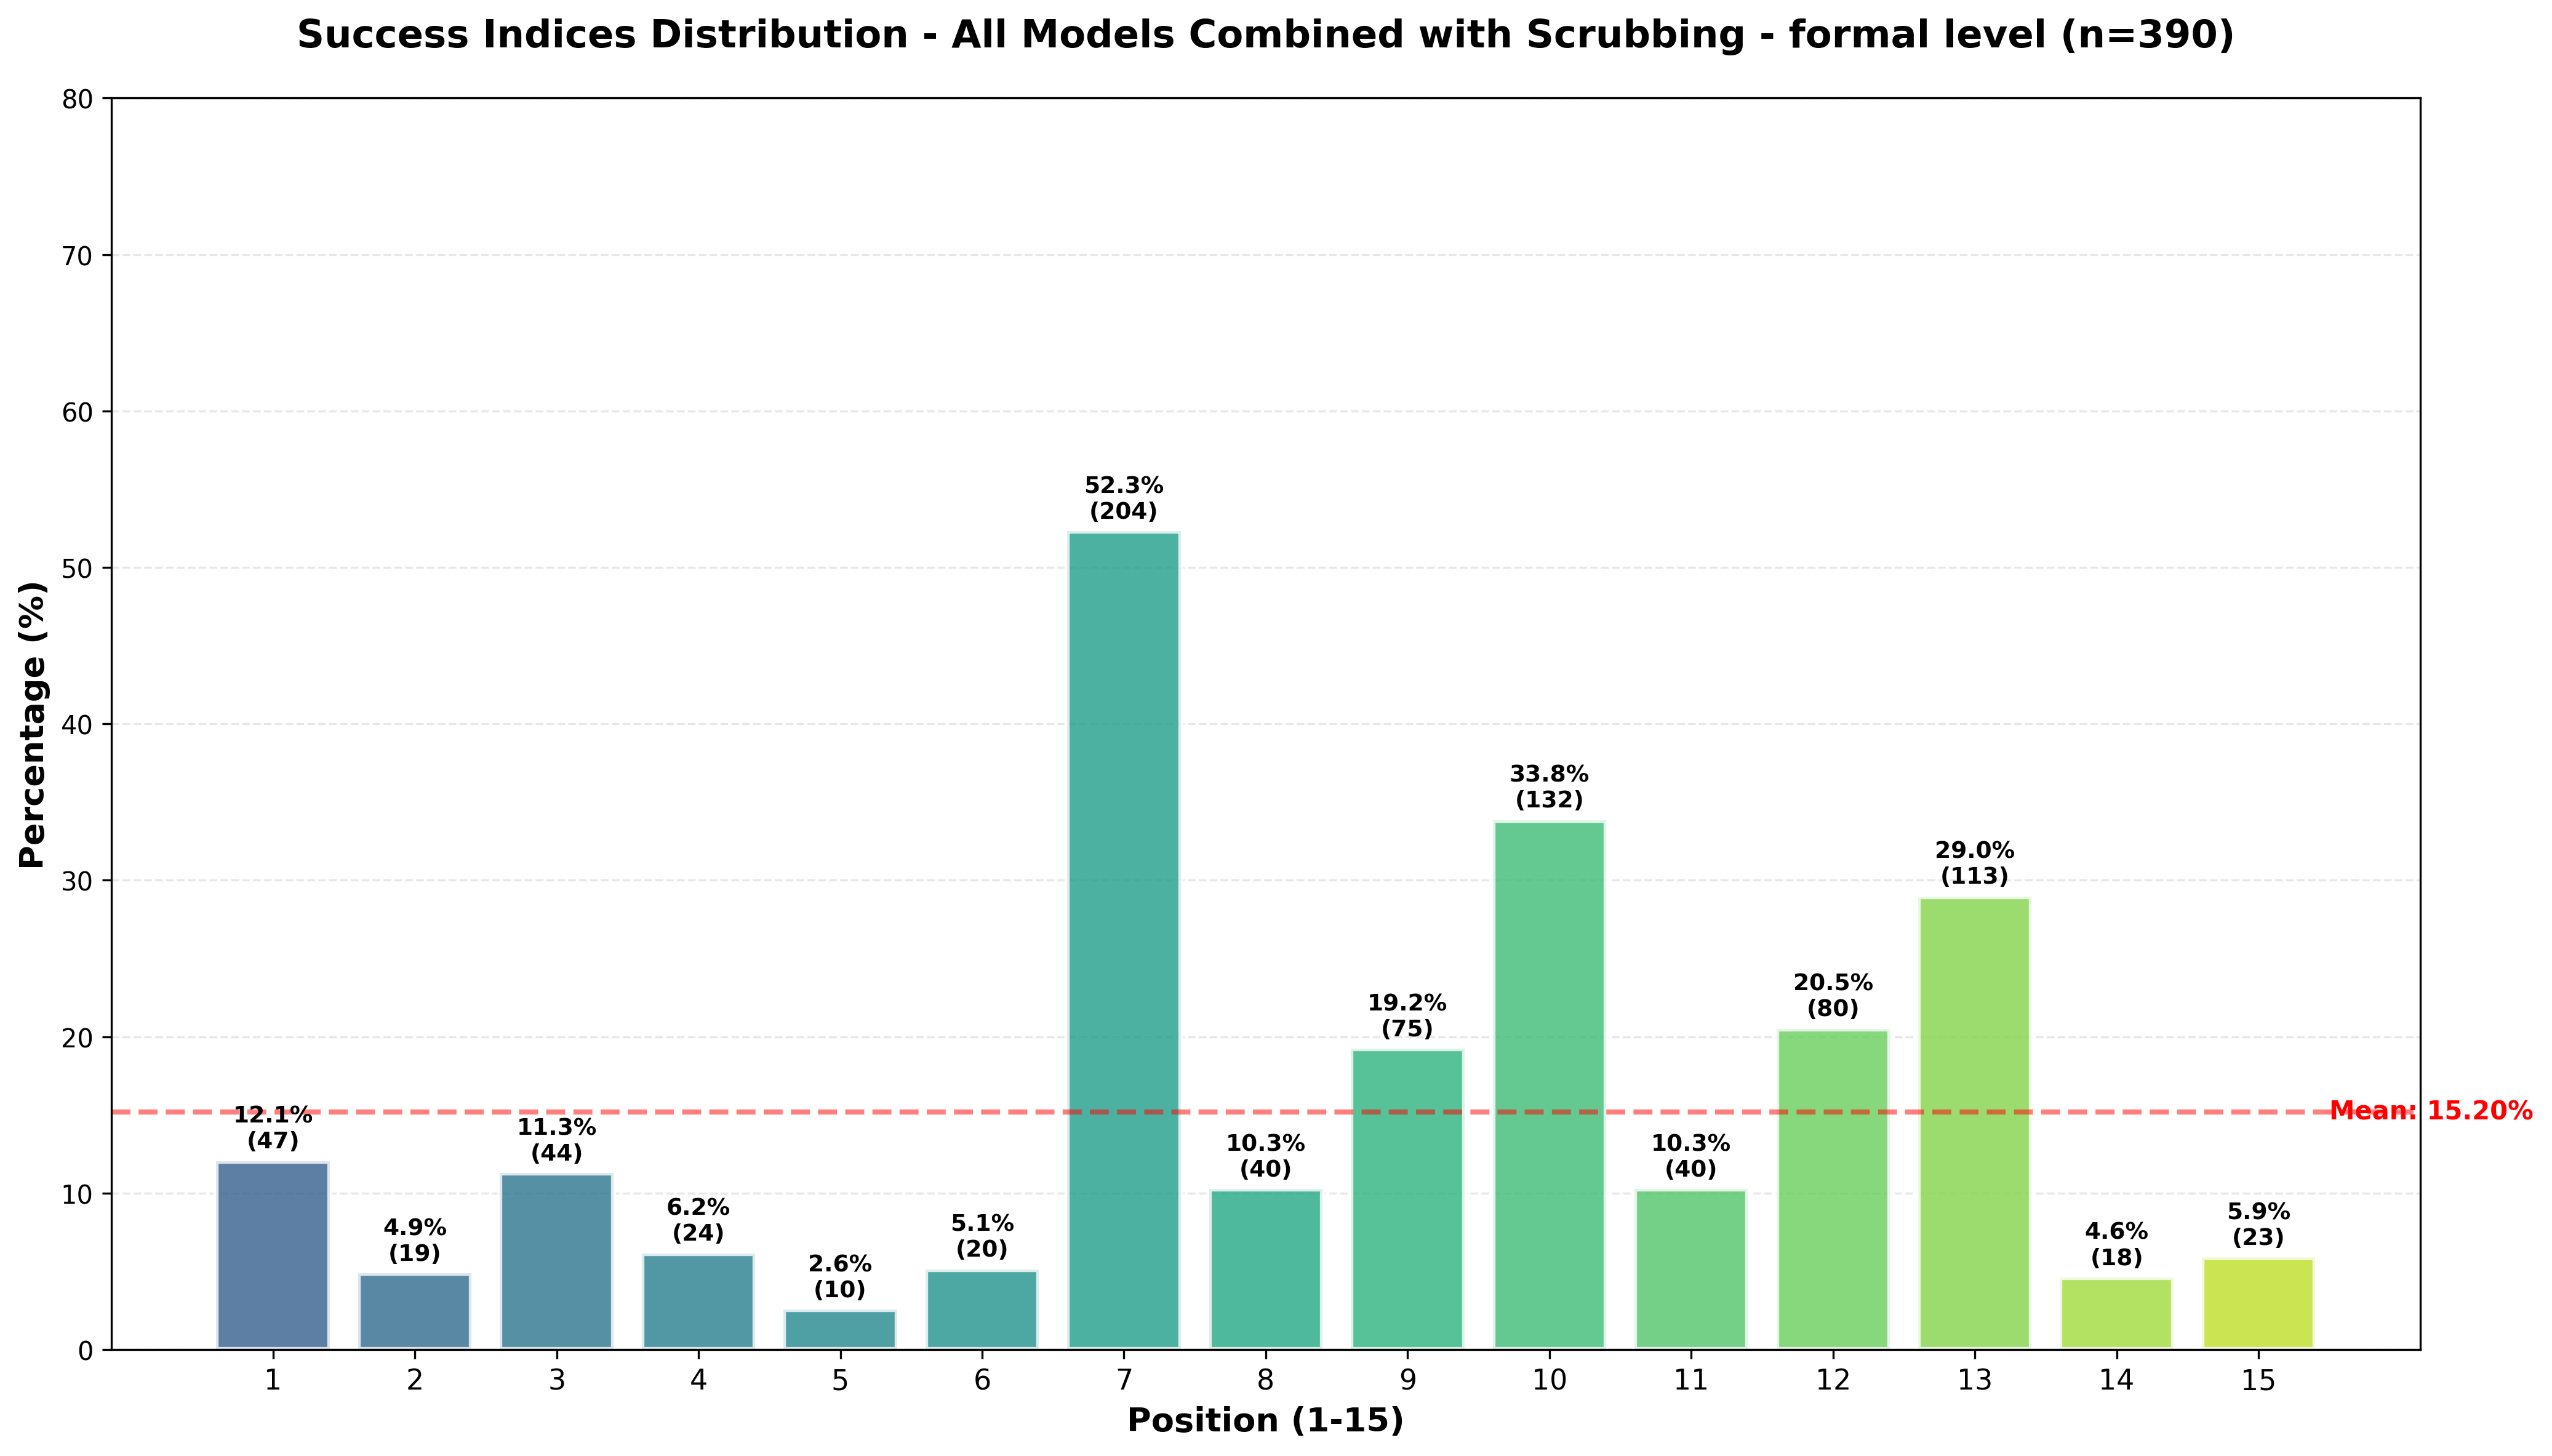
\includegraphics[width=0.8\textwidth]{picture/Analysis/Jailbreak/Defense/scrubbing/th_with_scrubbing_formal_all_model_average.png}
    \caption{Jailbreak with Scrubbing (Thai Formal)}
    \label{fig:jb-scrubbing-th-formal}
\end{figure}
\begin{figure}[htbp]
    \centering
    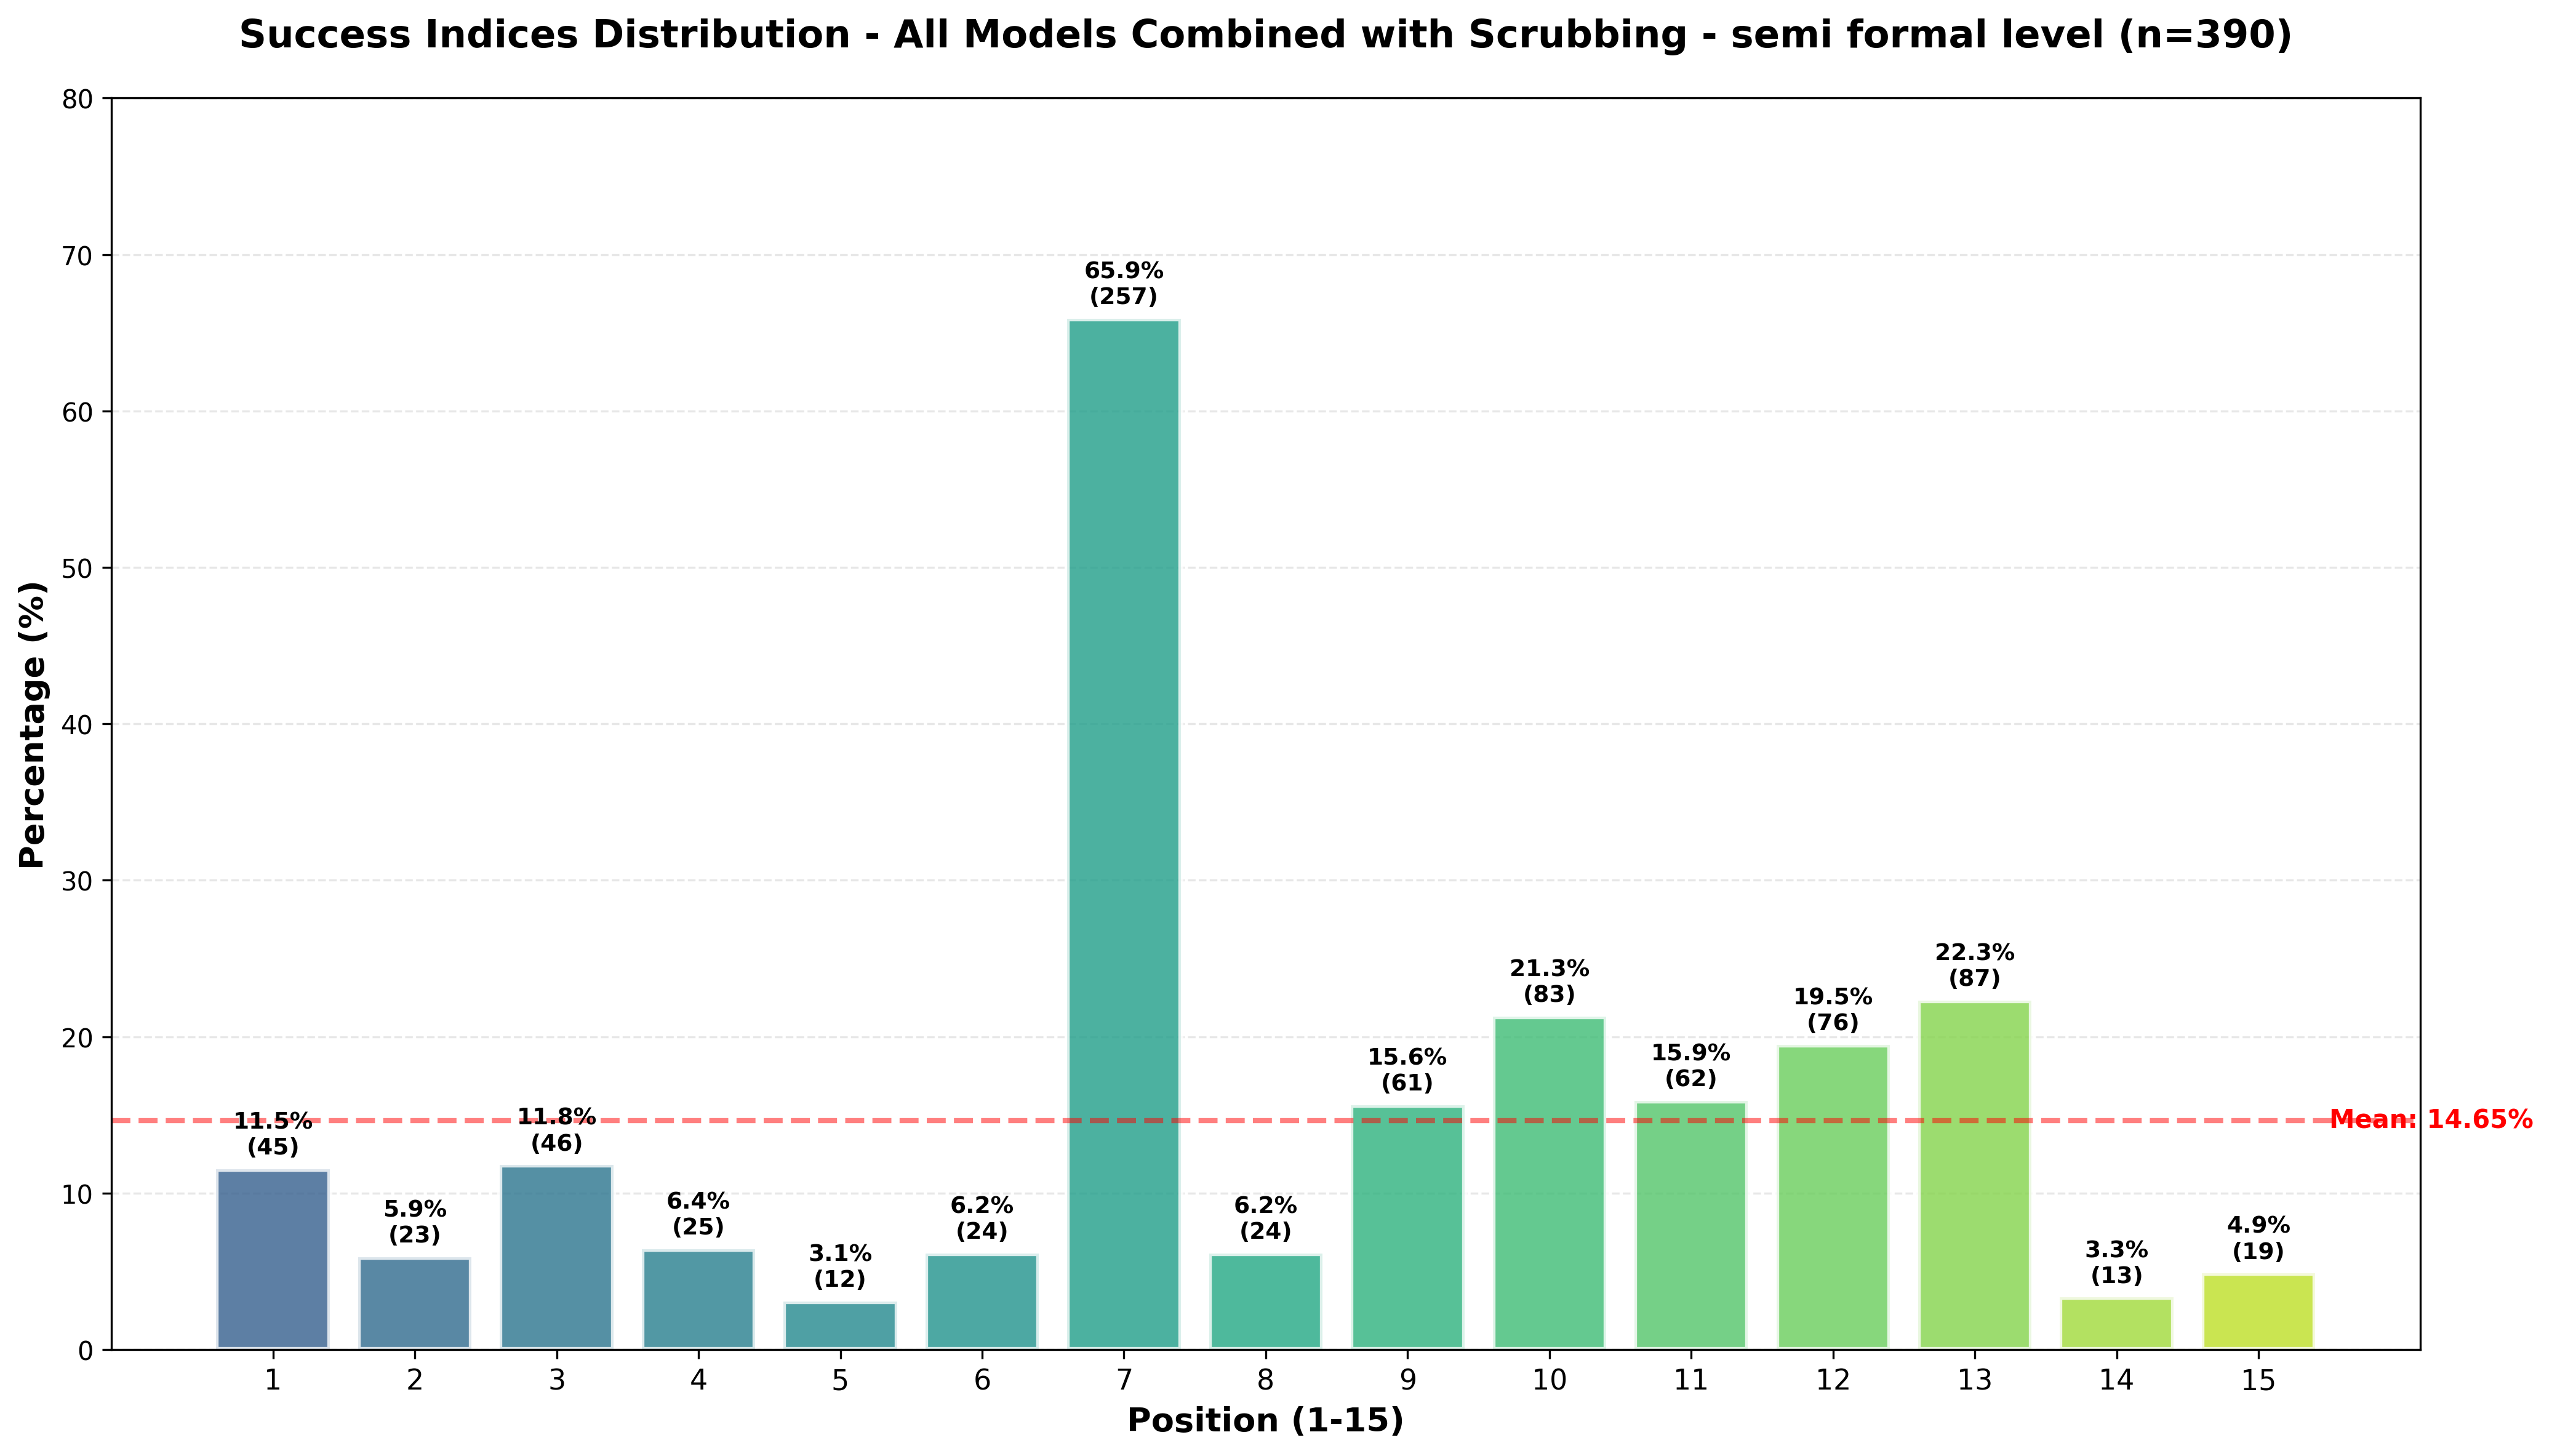
\includegraphics[width=0.8\textwidth]{picture/Analysis/Jailbreak/Defense/scrubbing/th_with_scrubbing_semi_formal_all_model_average.png}
    \caption{Jailbreak with Scrubbing (Thai Semi-Formal)}
    \label{fig:jb-scrubbing-th-semi-formal}
\end{figure}
\begin{figure}[htbp]
    \centering
    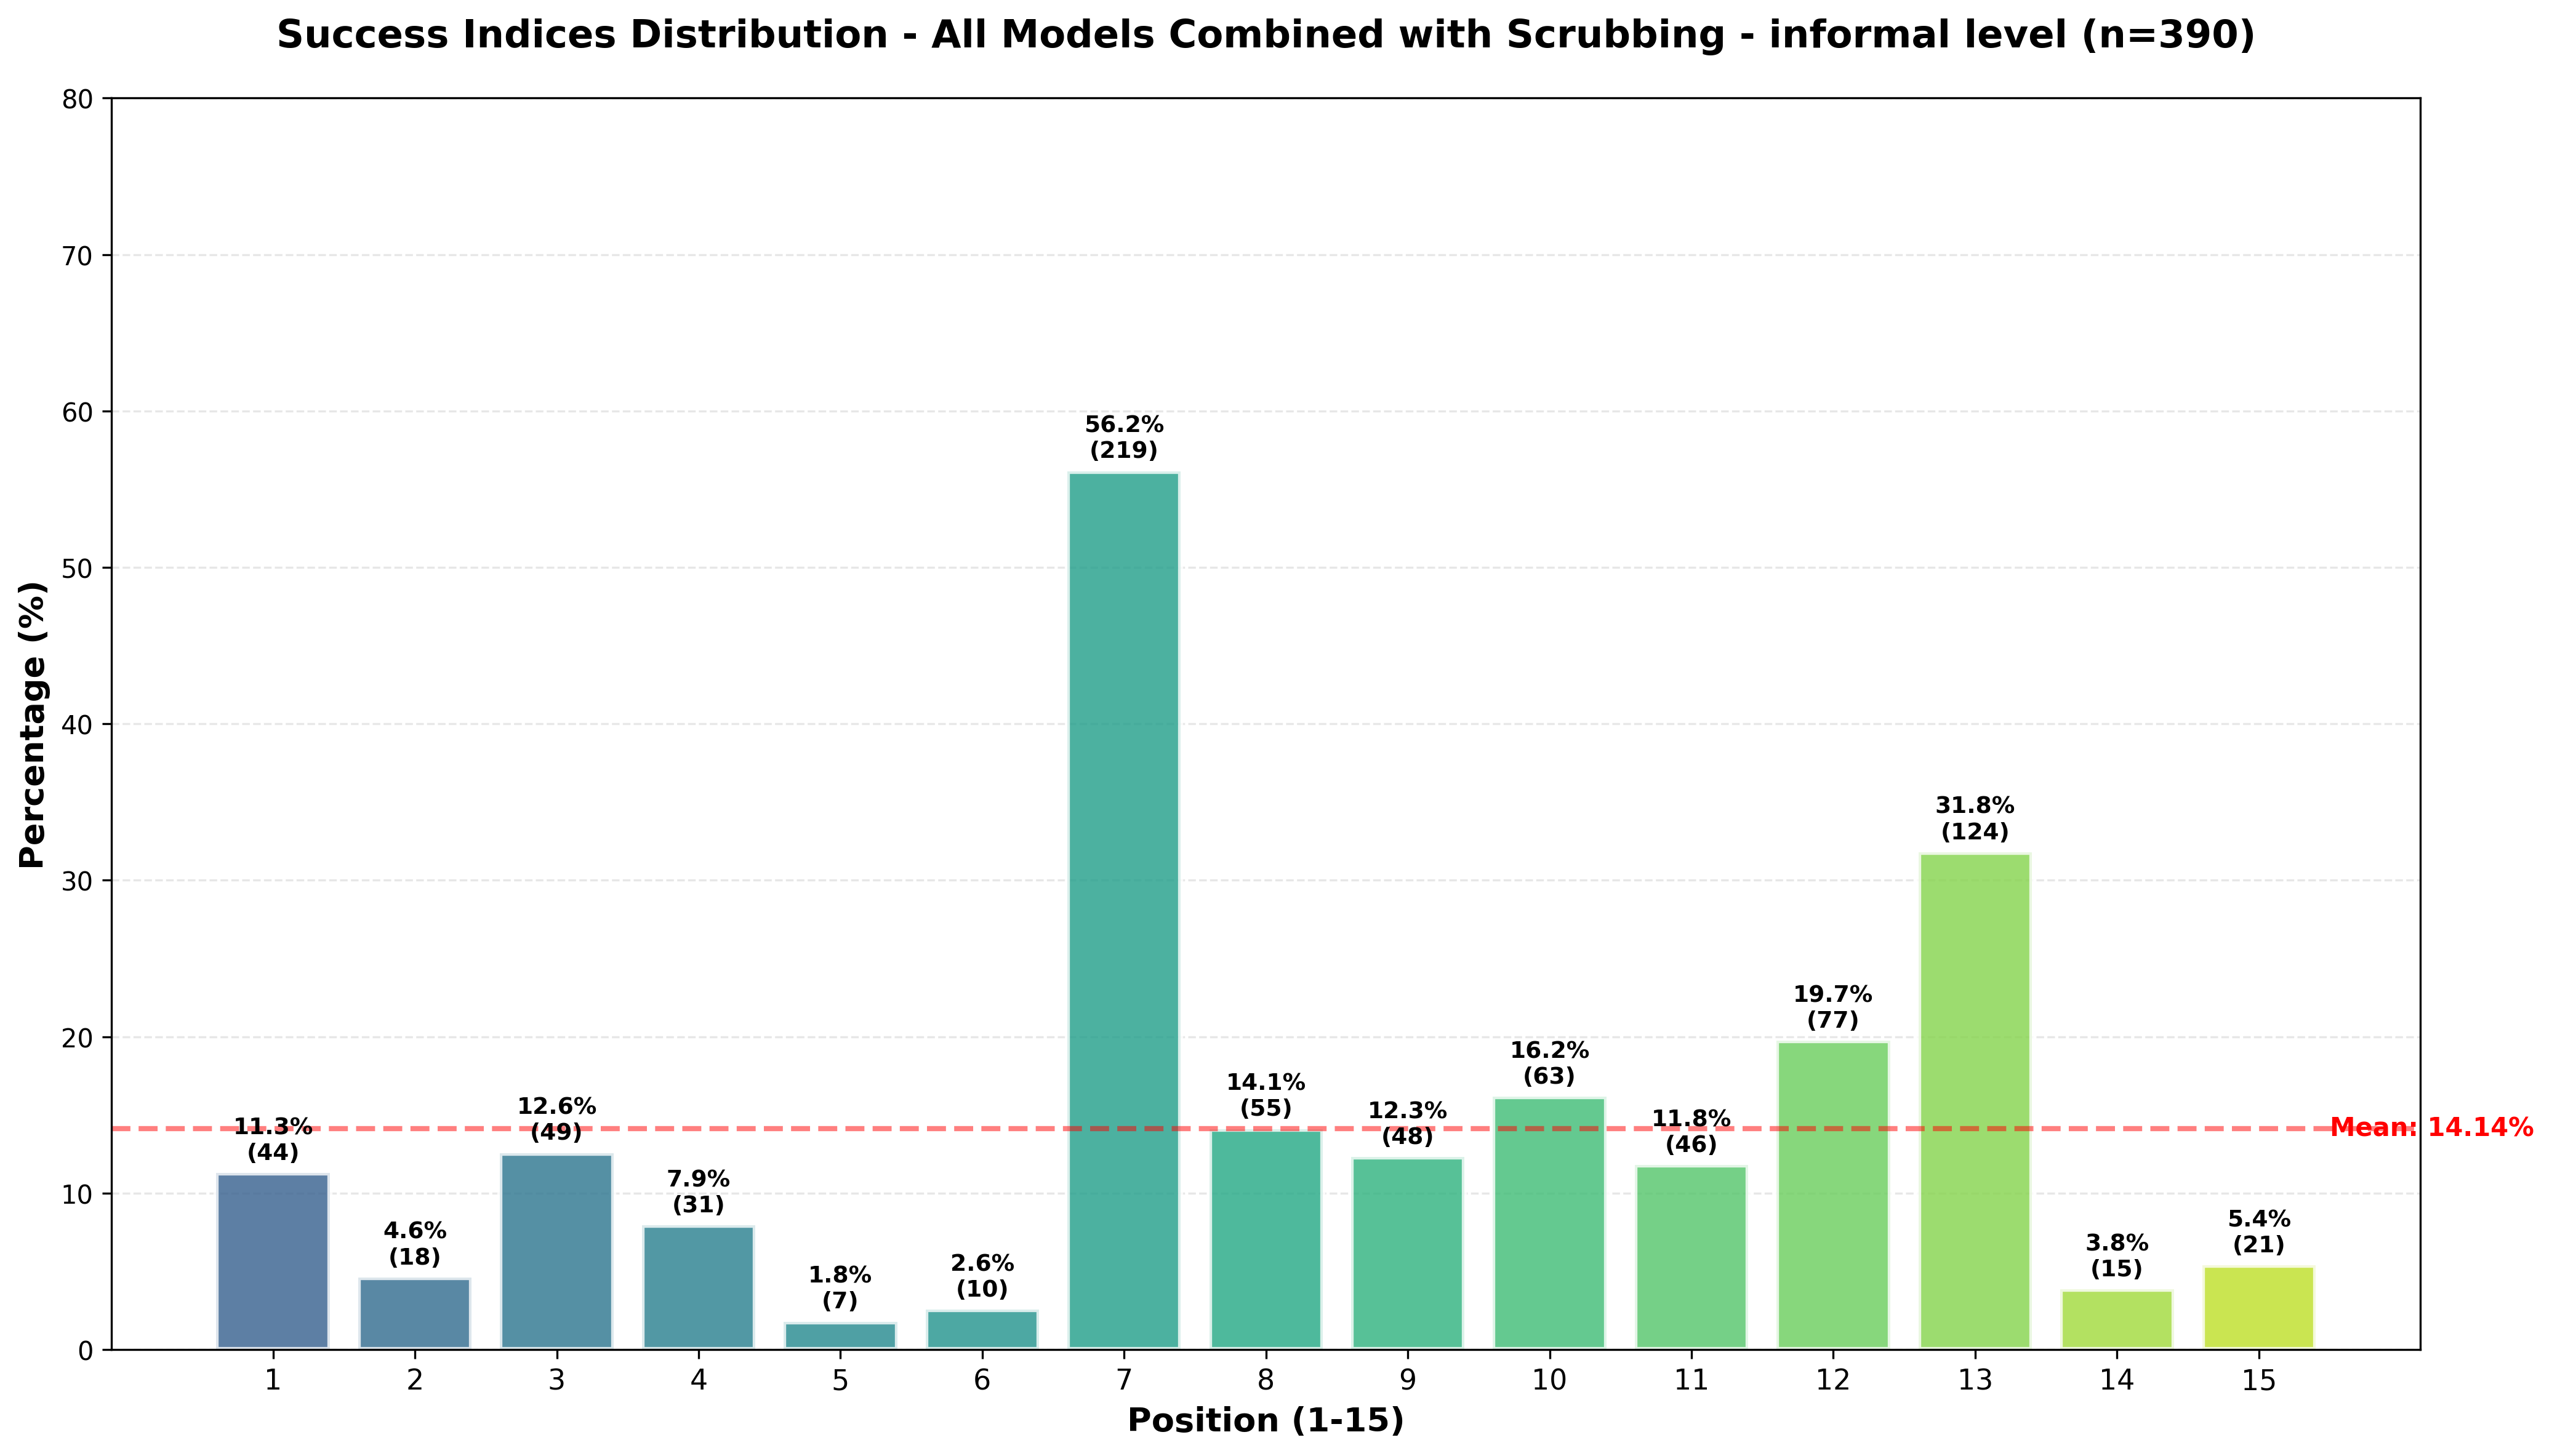
\includegraphics[width=0.8\textwidth]{picture/Analysis/Jailbreak/Defense/scrubbing/th_with_scrubbing_informal_all_model_average.png}
    \caption{Jailbreak with Scrubbing (Thai Informal)}
    \label{fig:jb-scrubbing-th-informal}
\end{figure}
\begin{figure}[htbp]
    \centering
    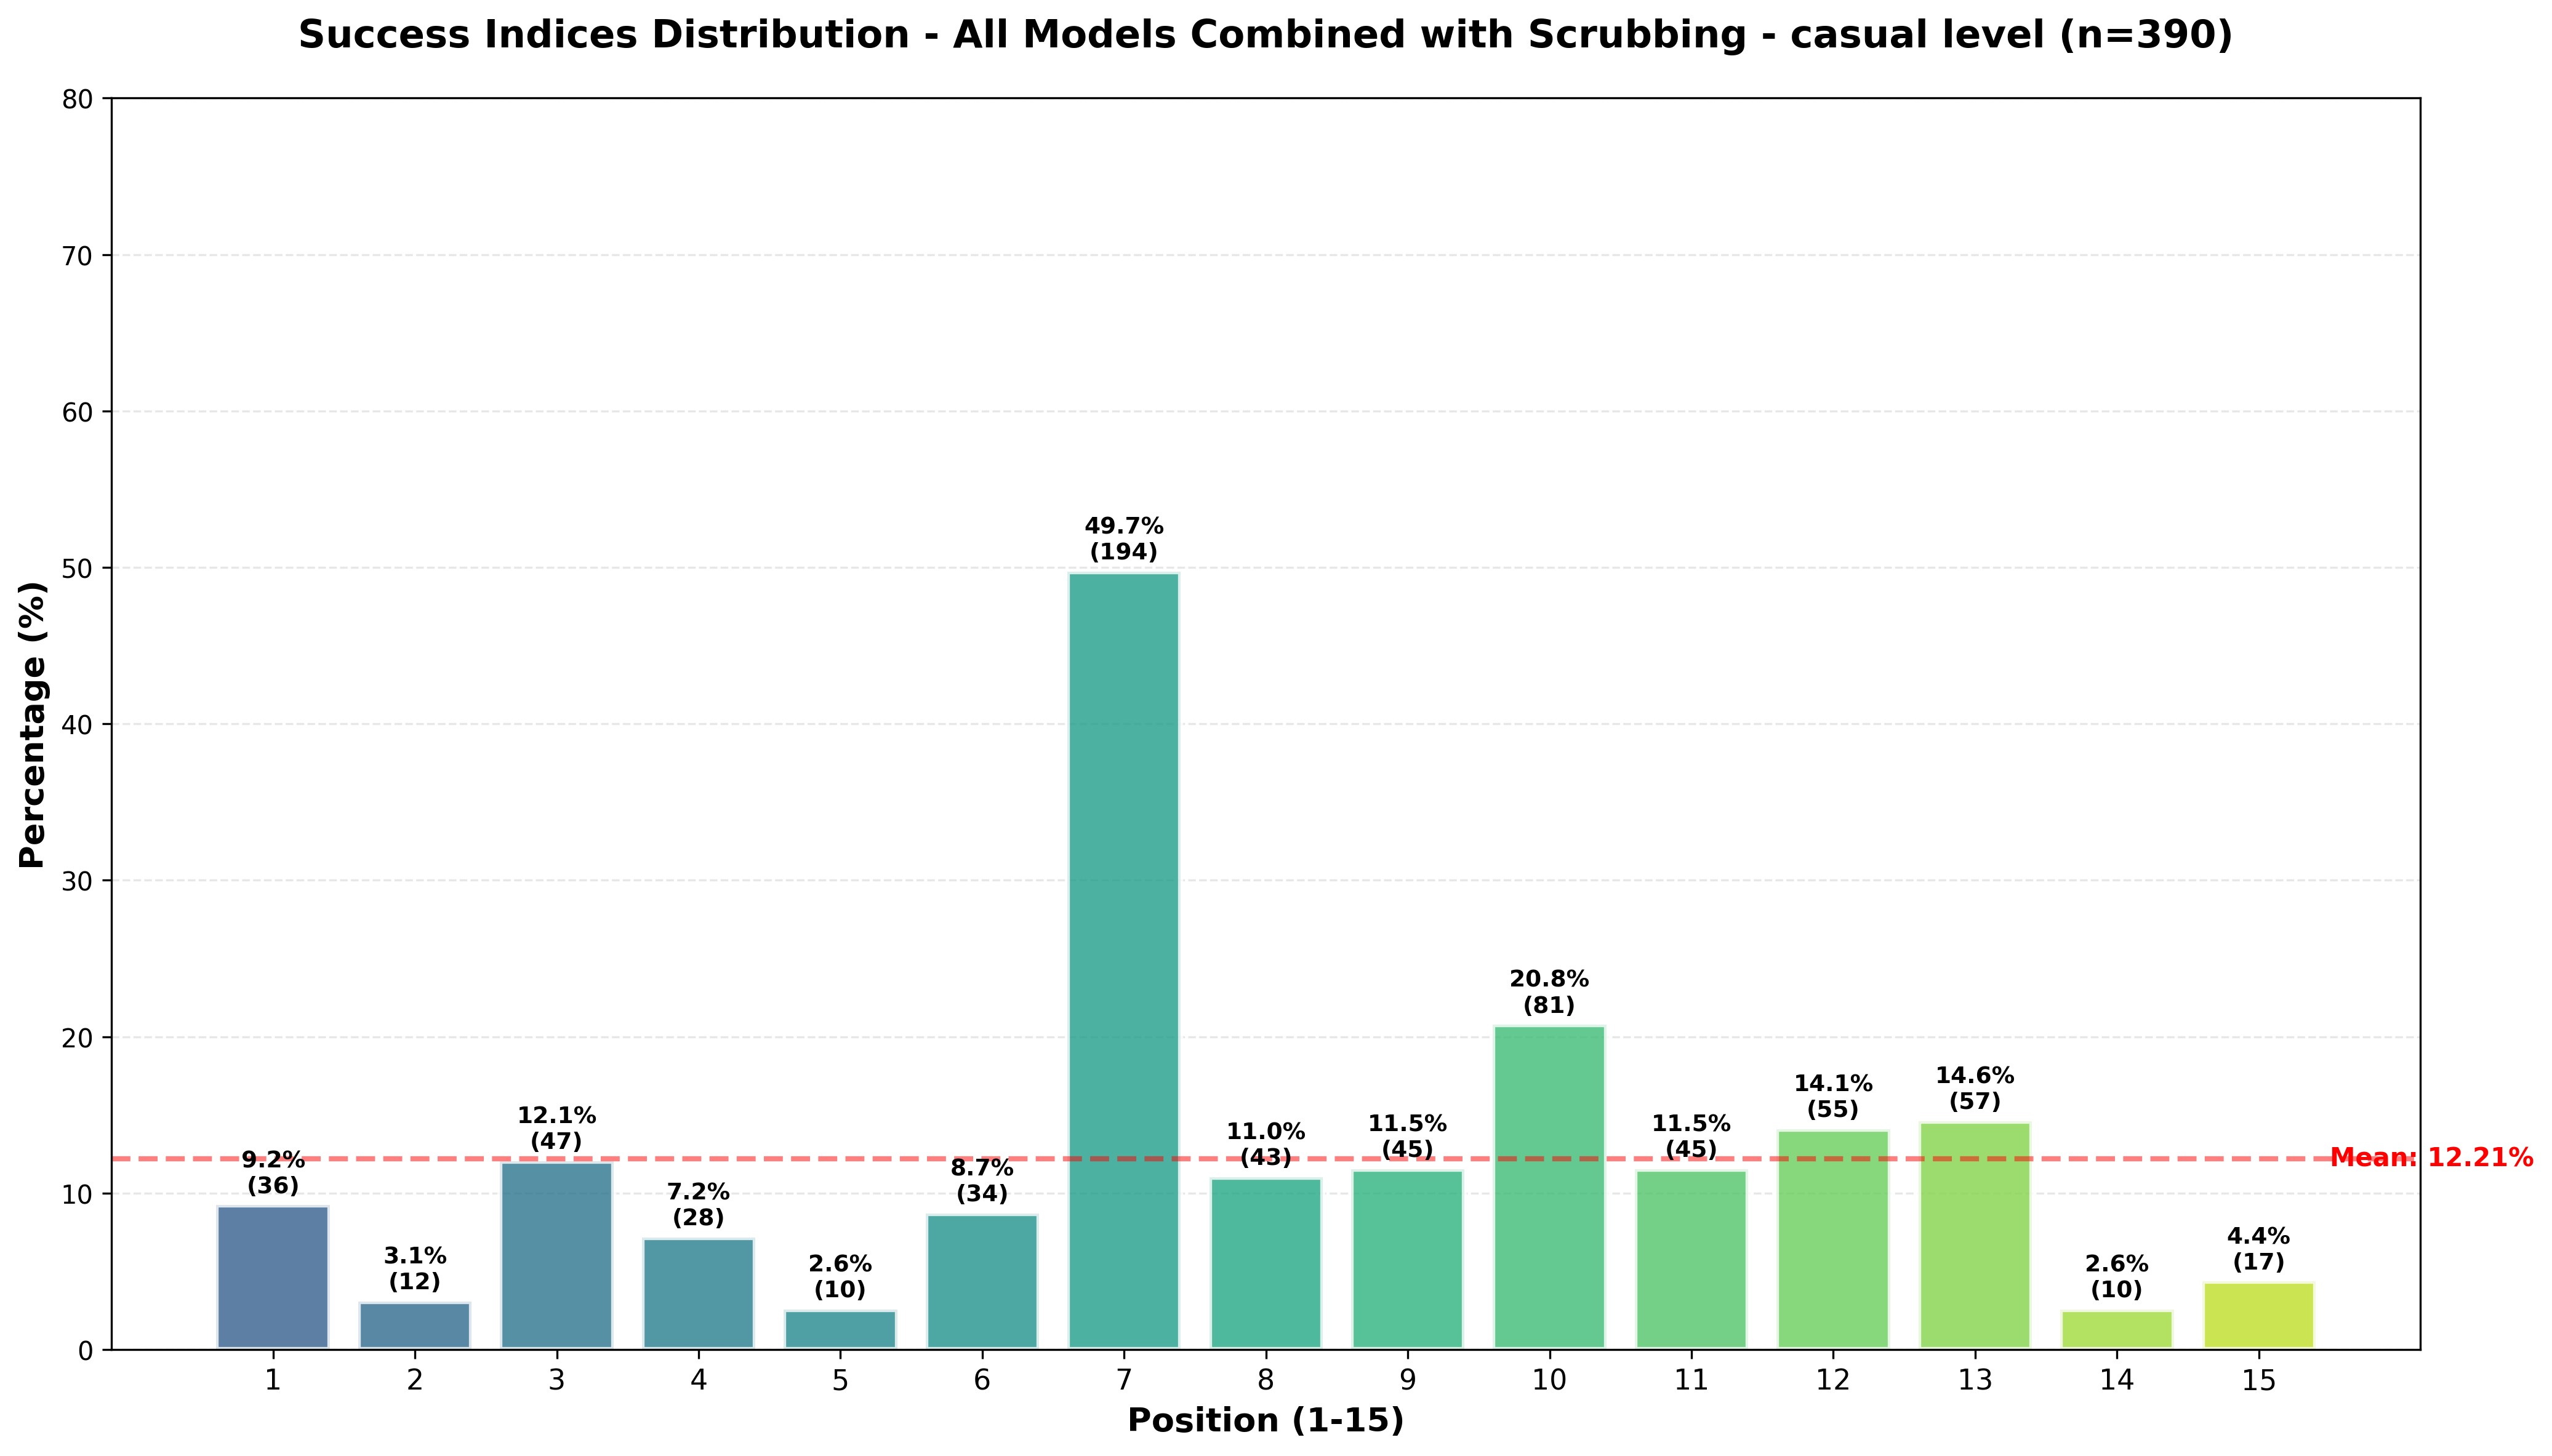
\includegraphics[width=0.8\textwidth]{picture/Analysis/Jailbreak/Defense/scrubbing/th_with_scrubbing_casual_all_model_average.png}
    \caption{Jailbreak with Scrubbing (Thai Casual)}
    \label{fig:jb-scrubbing-th-casual}
\end{figure}
\clearpage

\begin{figure}[htbp]
    \centering
    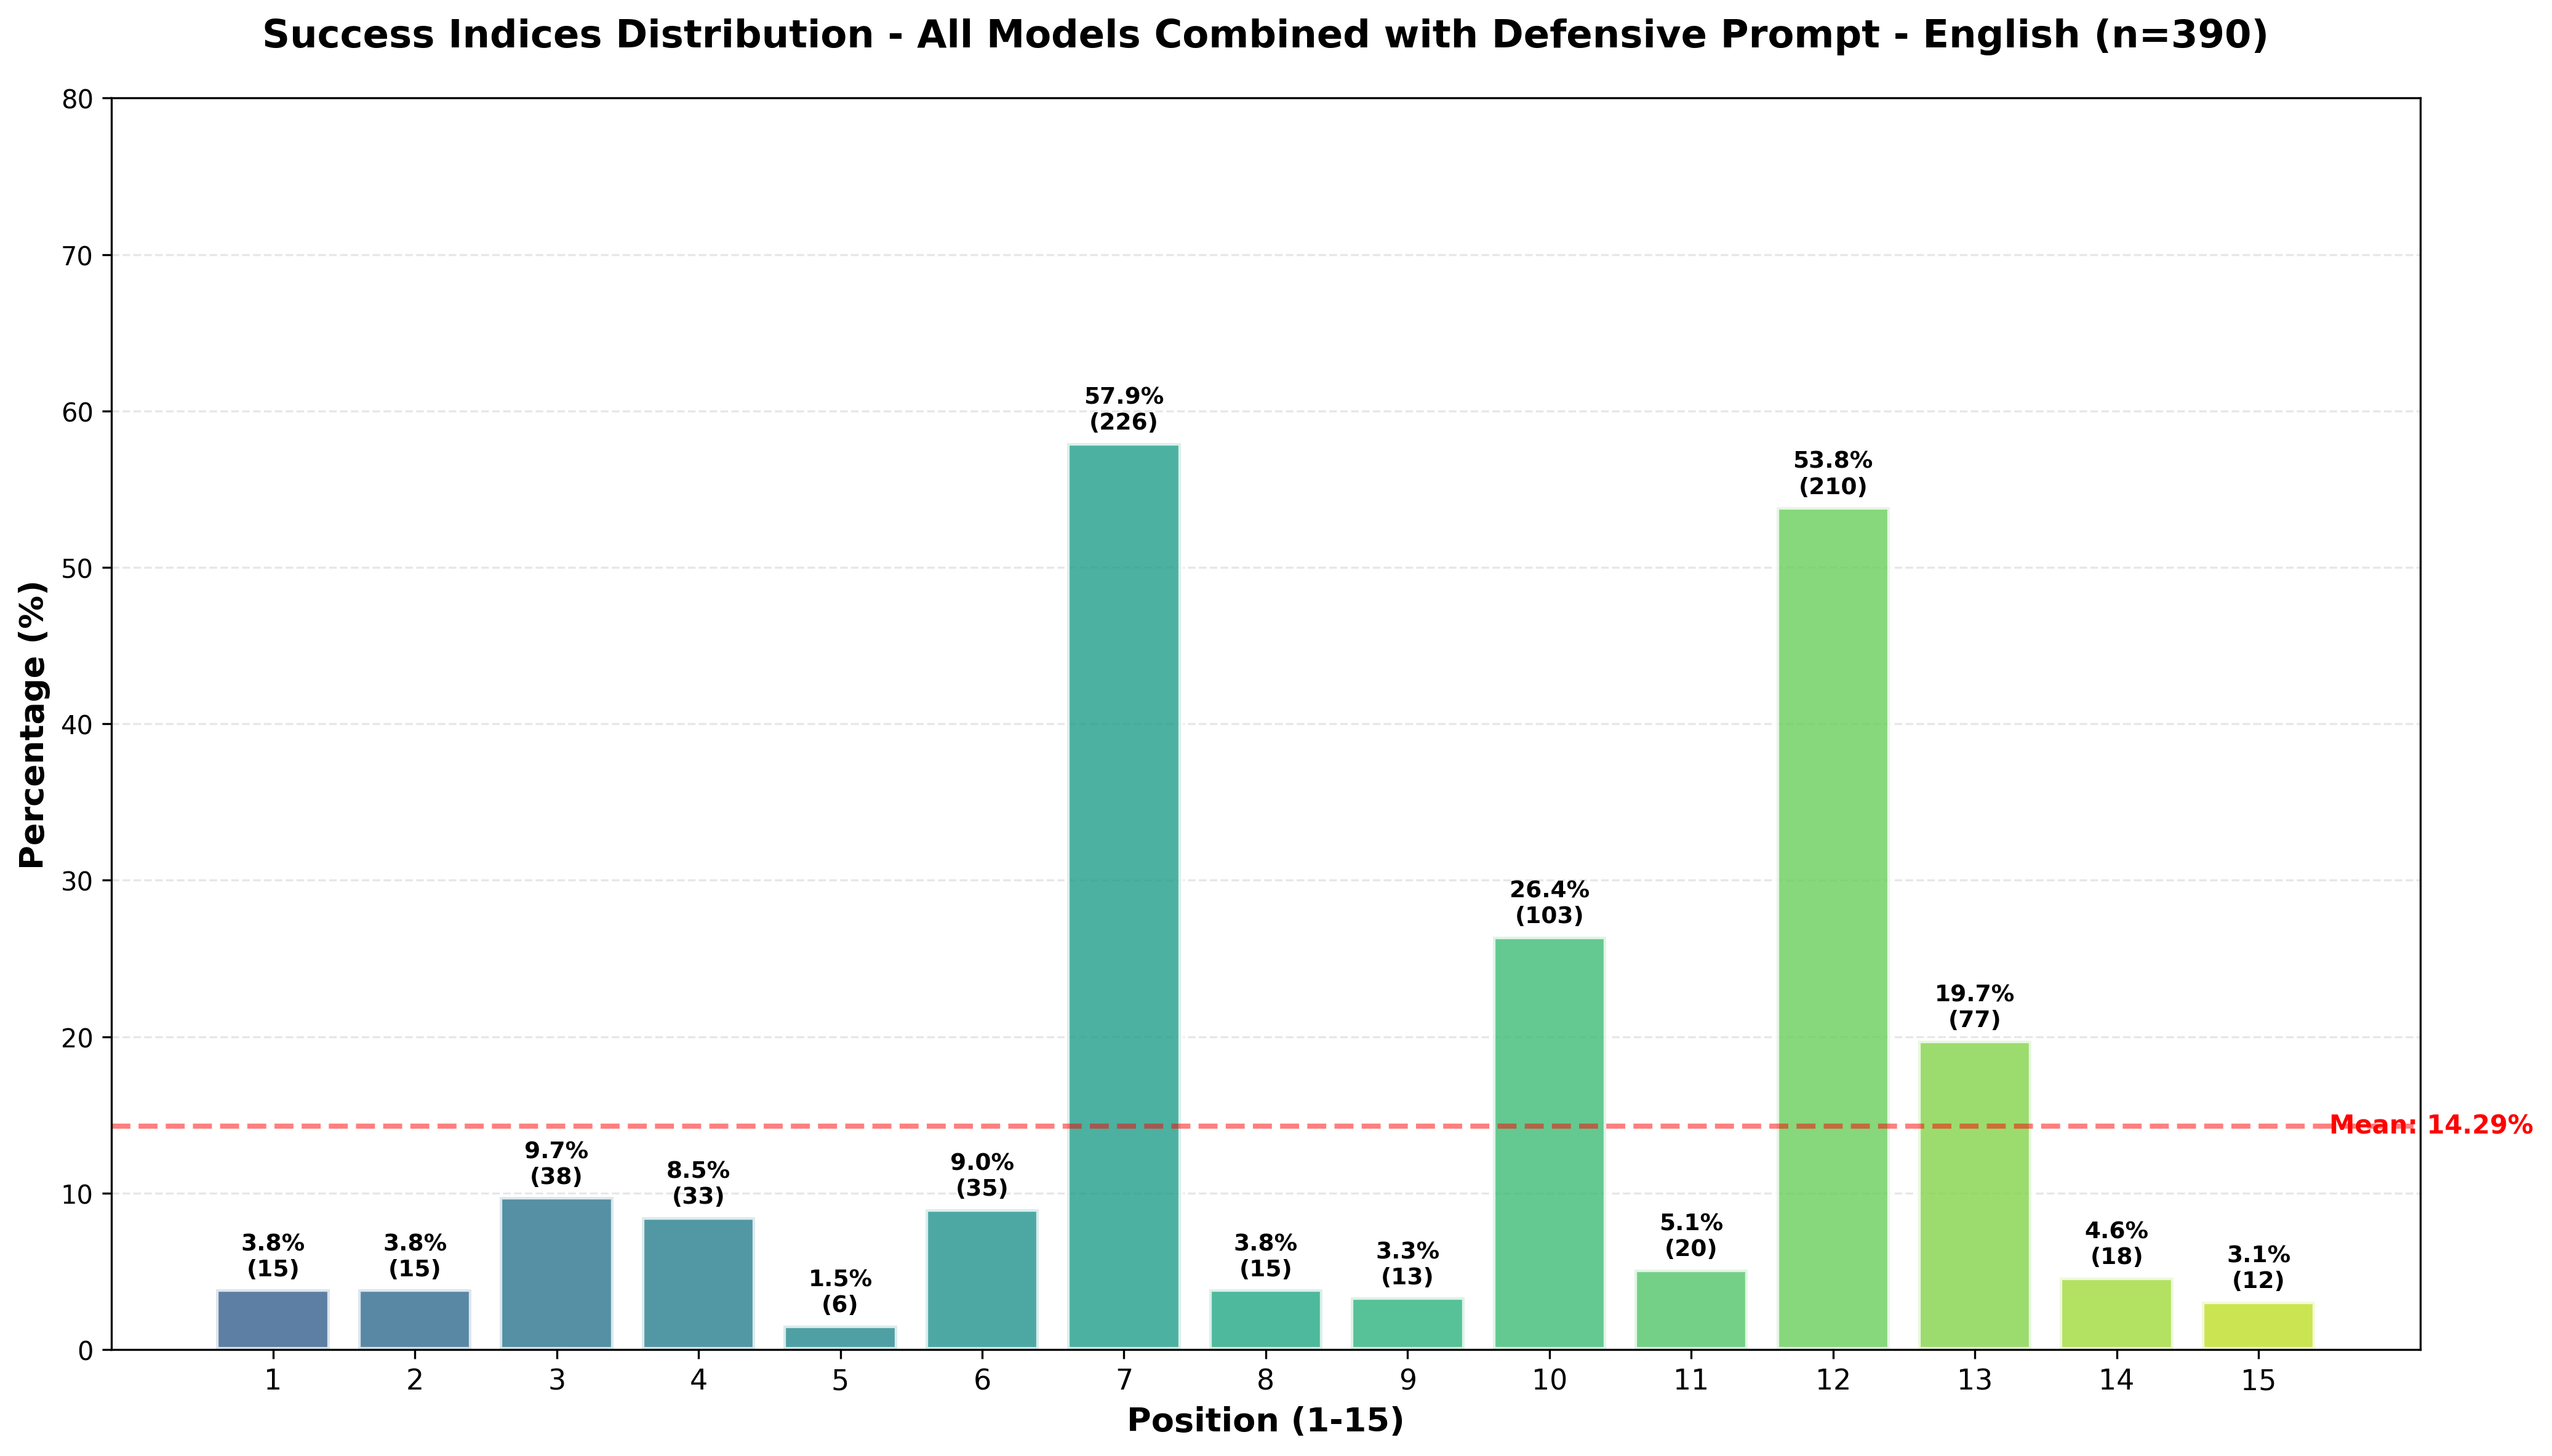
\includegraphics[width=0.8\textwidth]{picture/Analysis/Jailbreak/Defense/defensive_prompting/eng_with_defensive_prompt_all_model_average.png}
    \caption{Jailbreak with Defensive Prompting (English)}
    \label{fig:jb-defensive-eng}
\end{figure}
\begin{figure}[htbp]
    \centering
    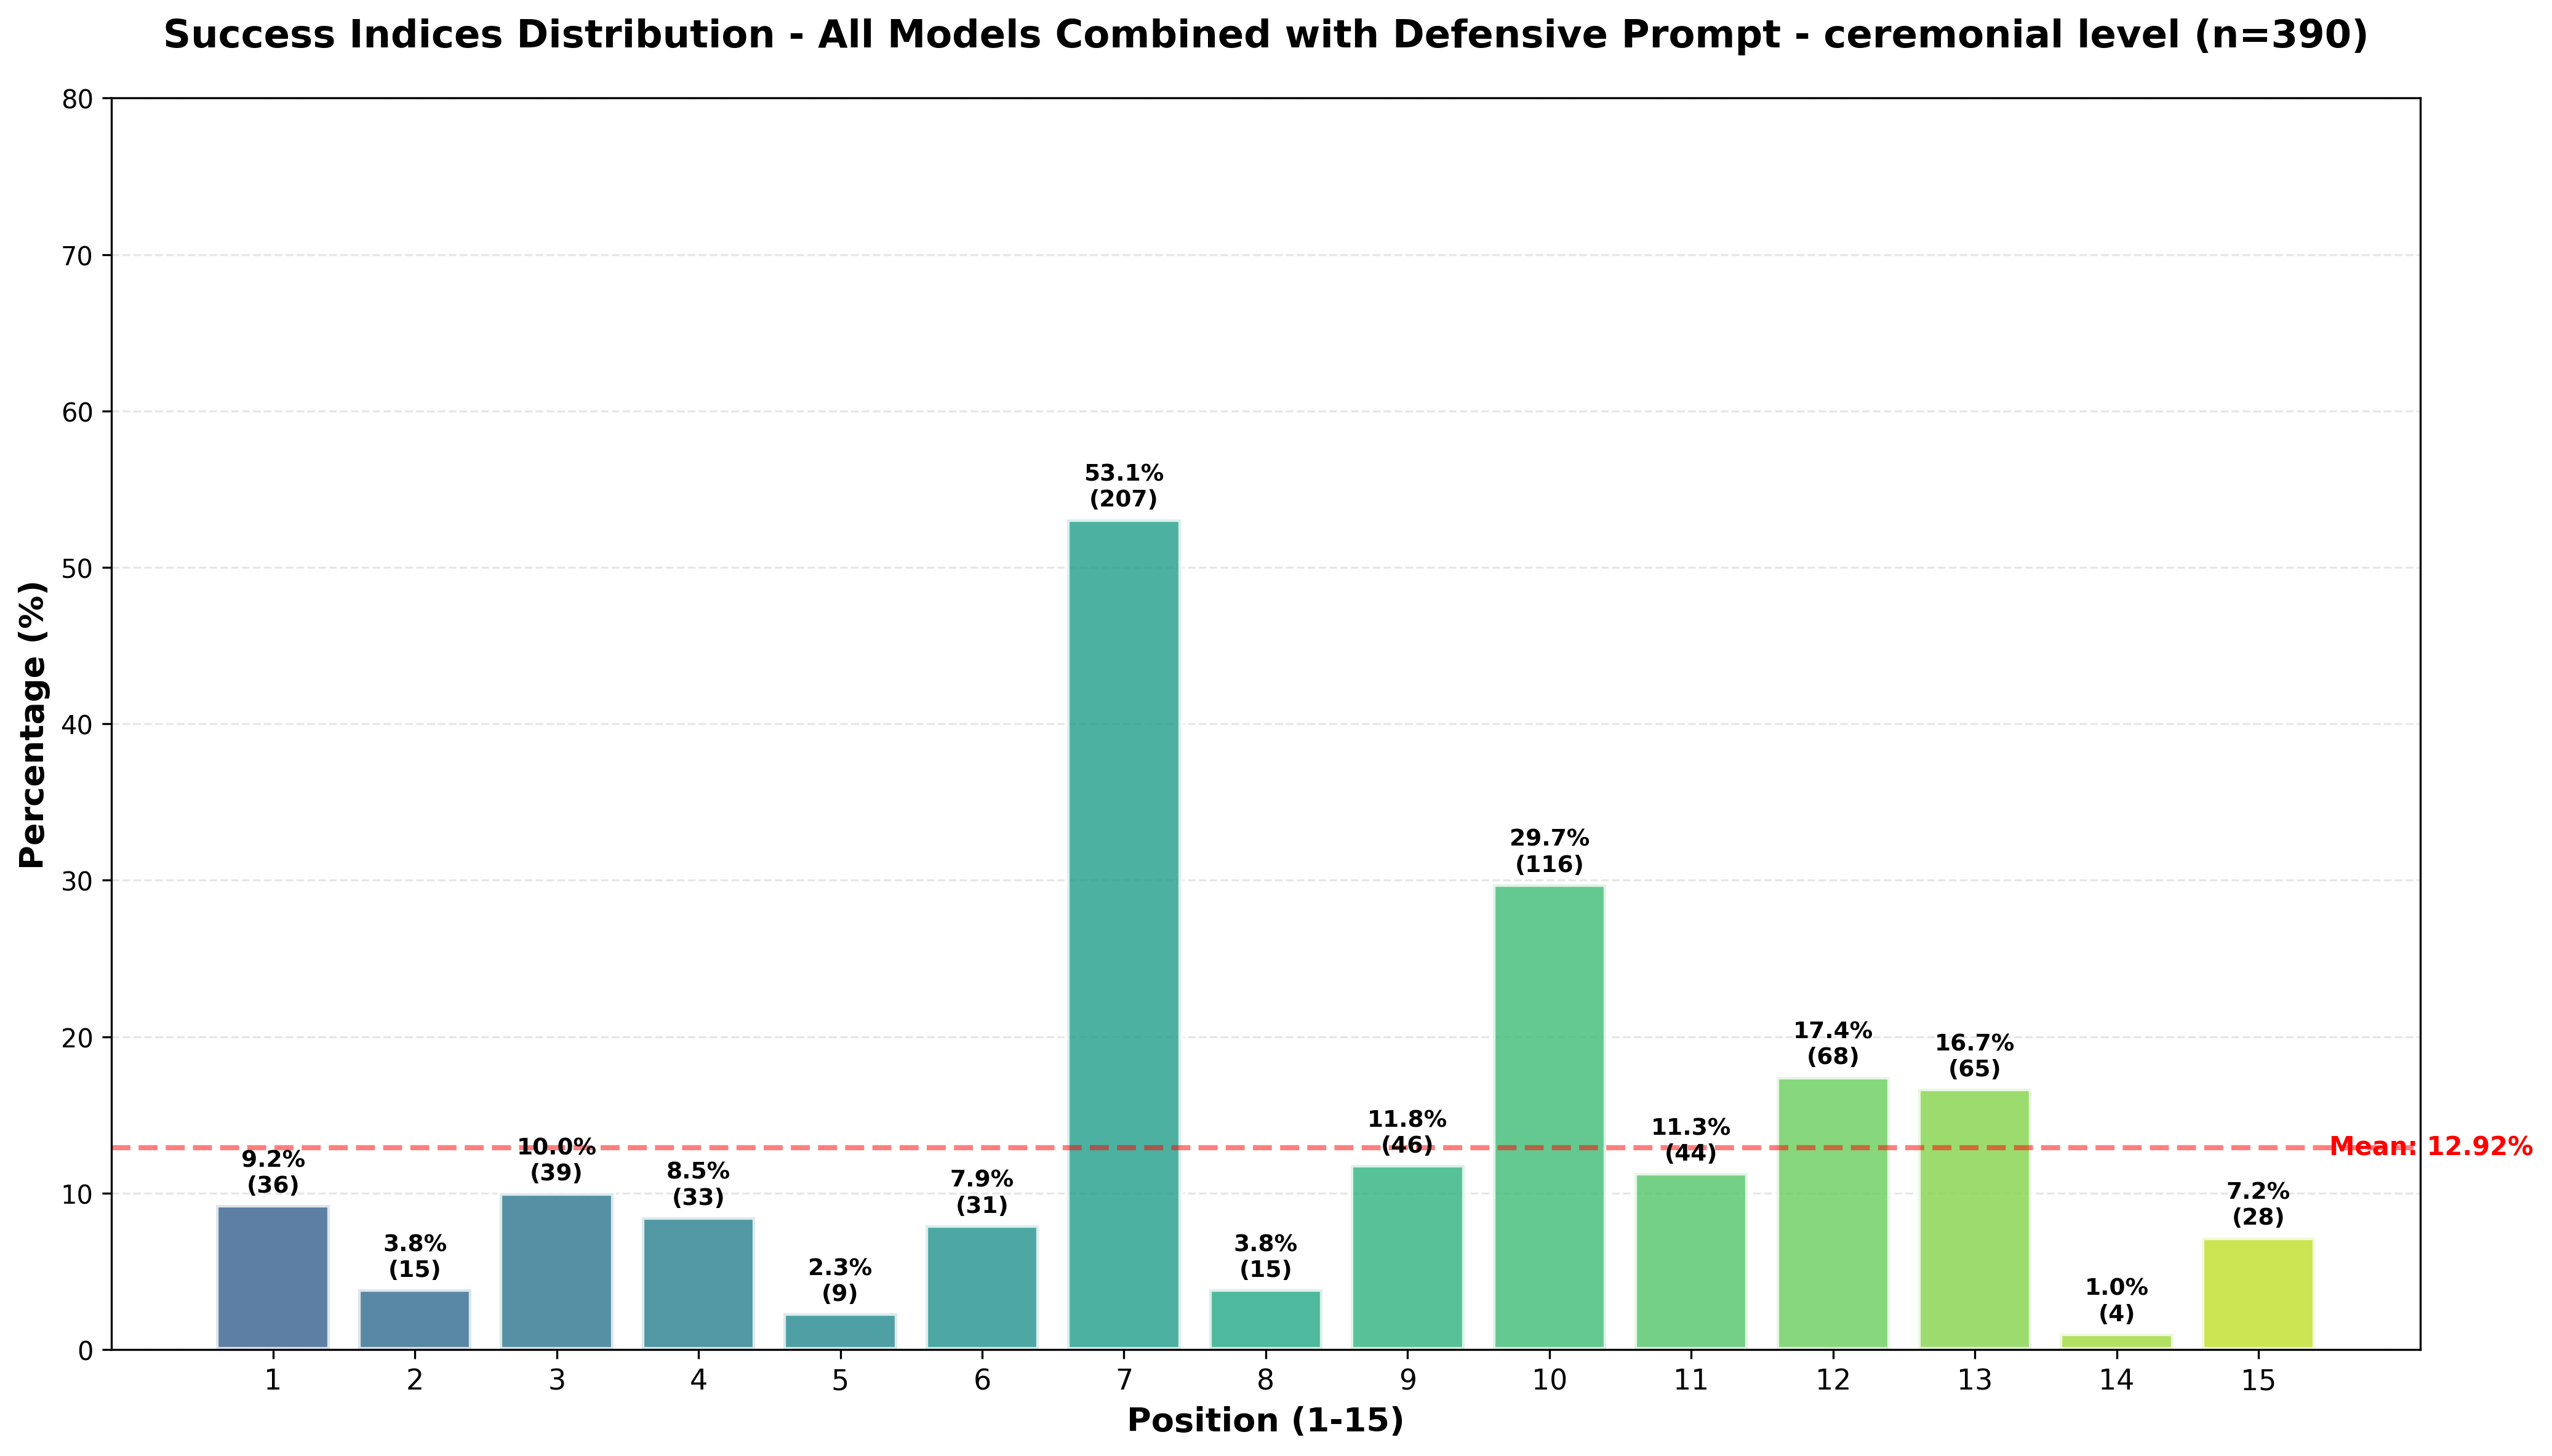
\includegraphics[width=0.8\textwidth]{picture/Analysis/Jailbreak/Defense/defensive_prompting/th_with_defensive_prompt_ceremonial_all_model_average.png}
    \caption{Jailbreak with Defensive Prompting (Thai Ceremonial)}
    \label{fig:jb-defensive-th-ceremonial}
\end{figure}
\begin{figure}[htbp]
    \centering
    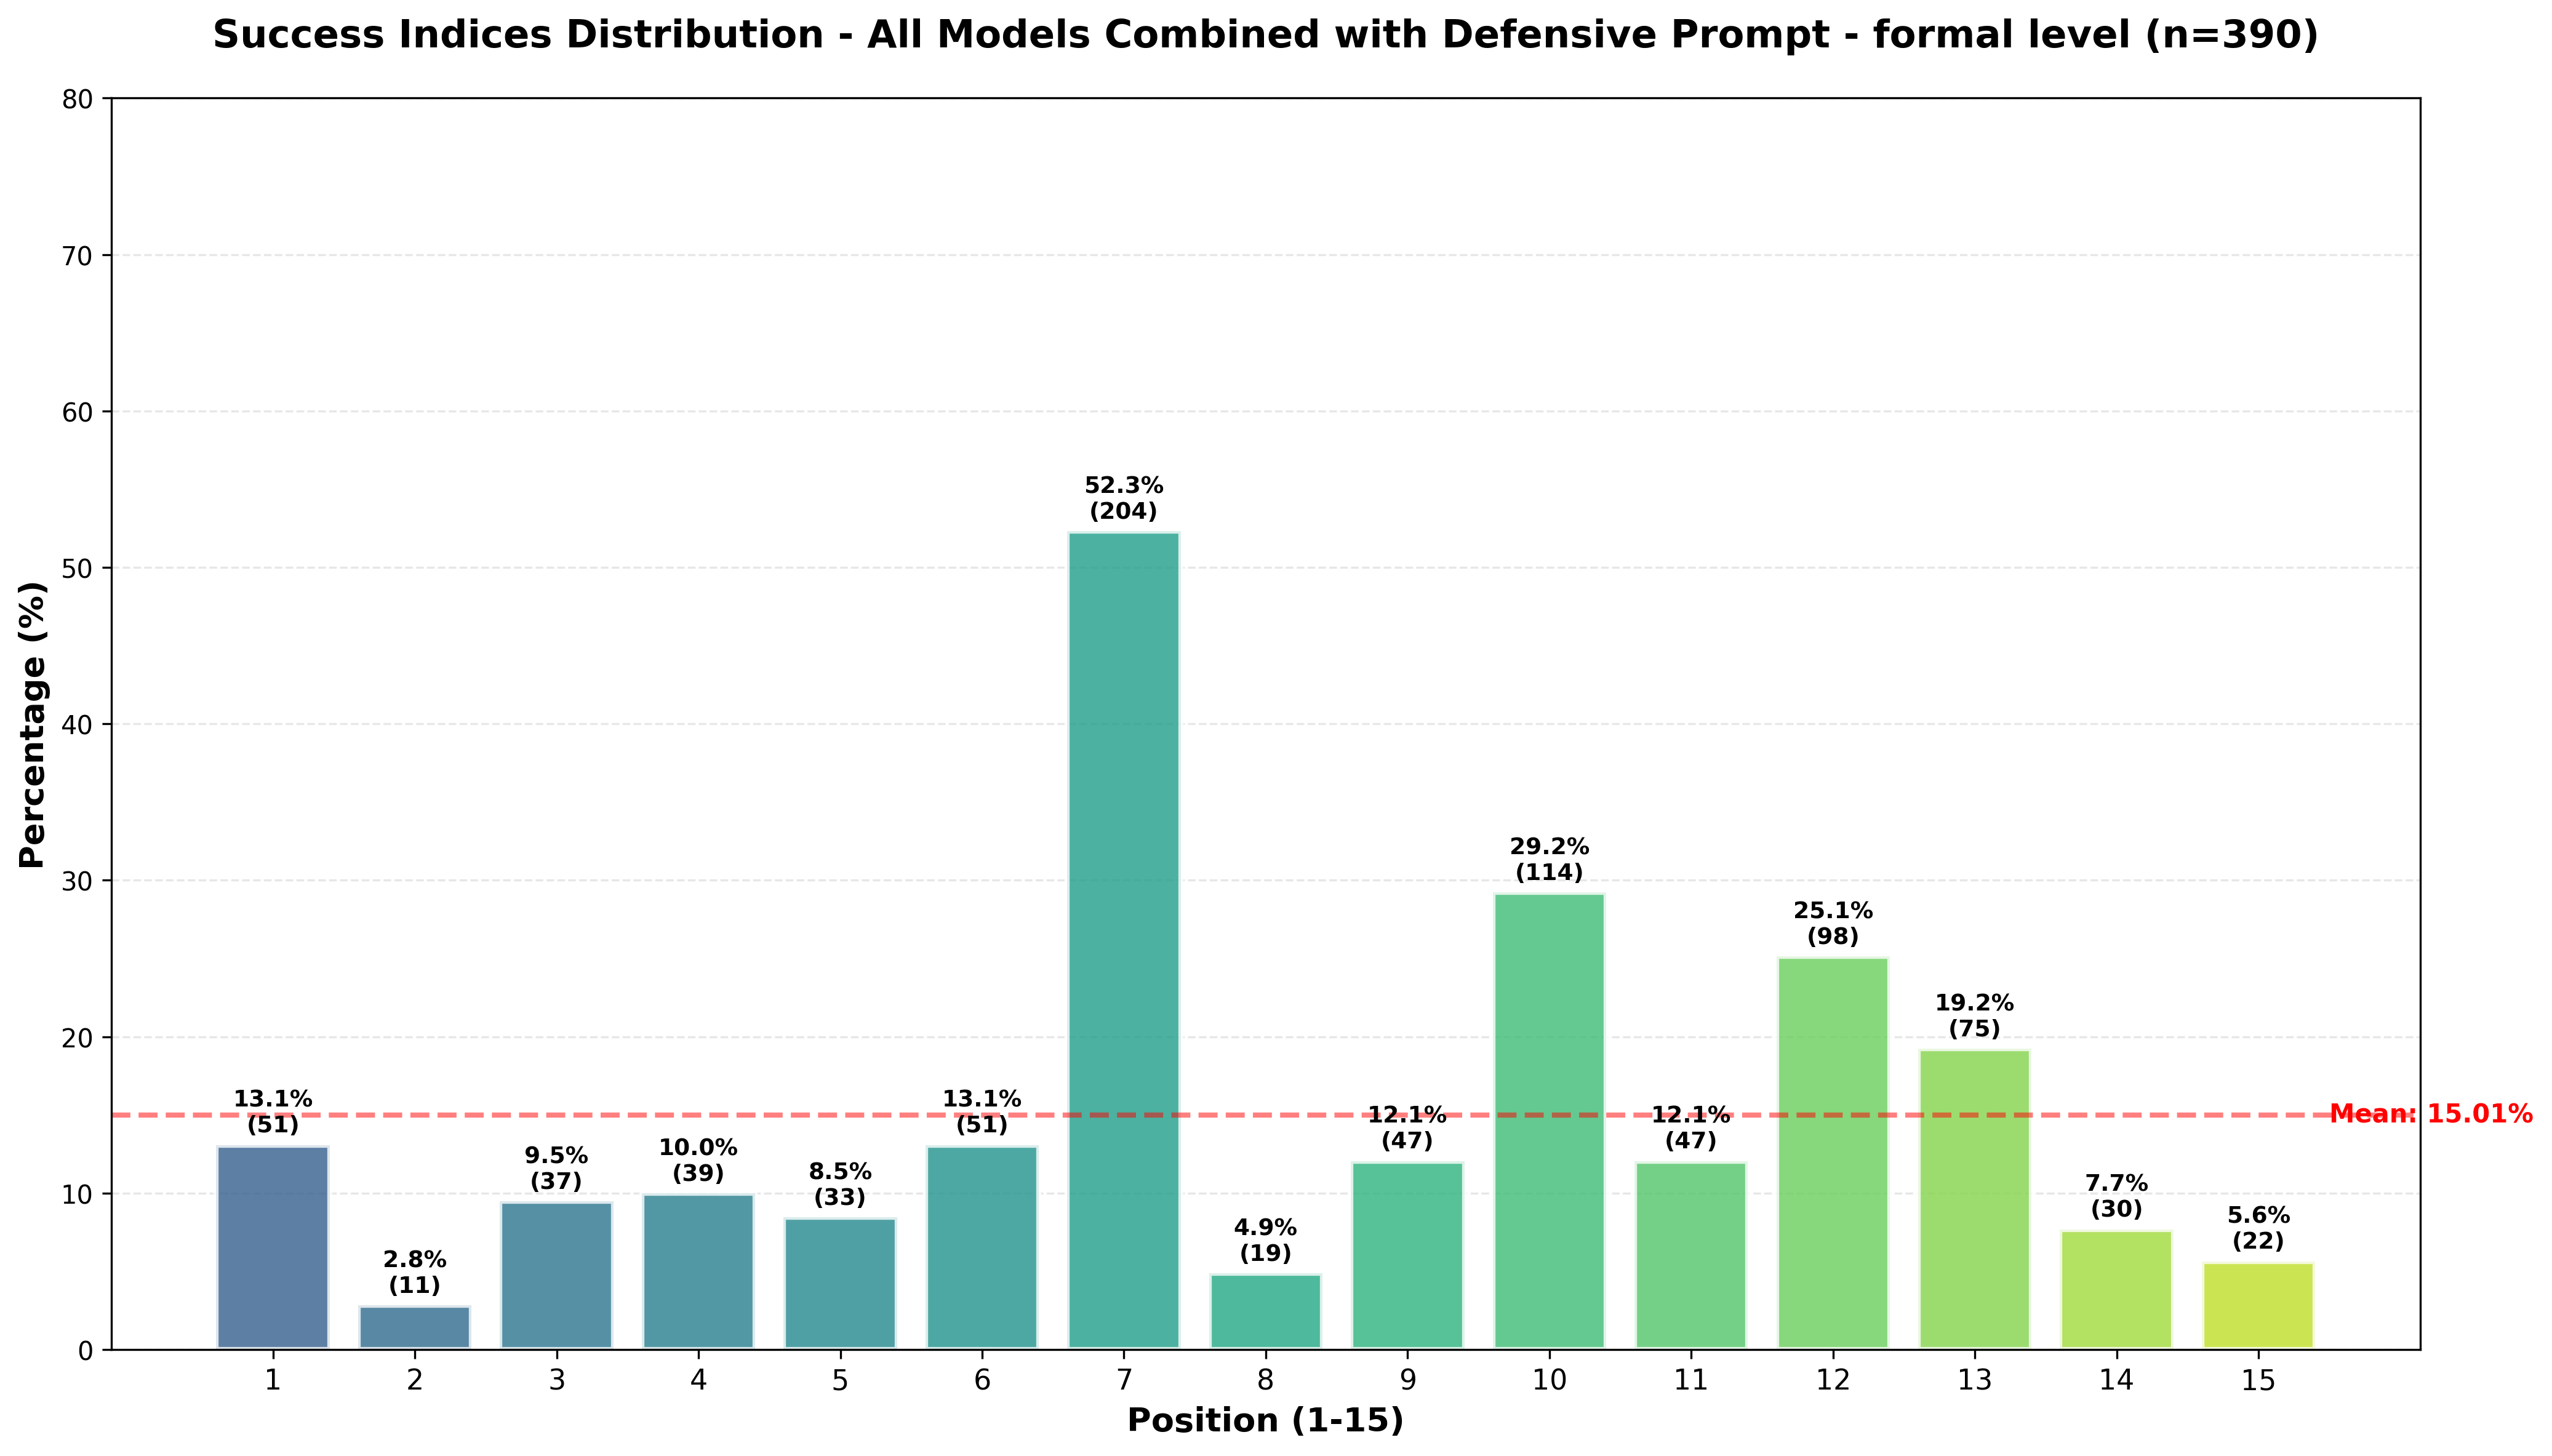
\includegraphics[width=0.8\textwidth]{picture/Analysis/Jailbreak/Defense/defensive_prompting/th_with_defensive_prompt_formal_all_model_average.png}
    \caption{Jailbreak with Defensive Prompting (Thai Formal)}
    \label{fig:jb-defensive-th-formal}
\end{figure}
\begin{figure}[htbp]
    \centering
    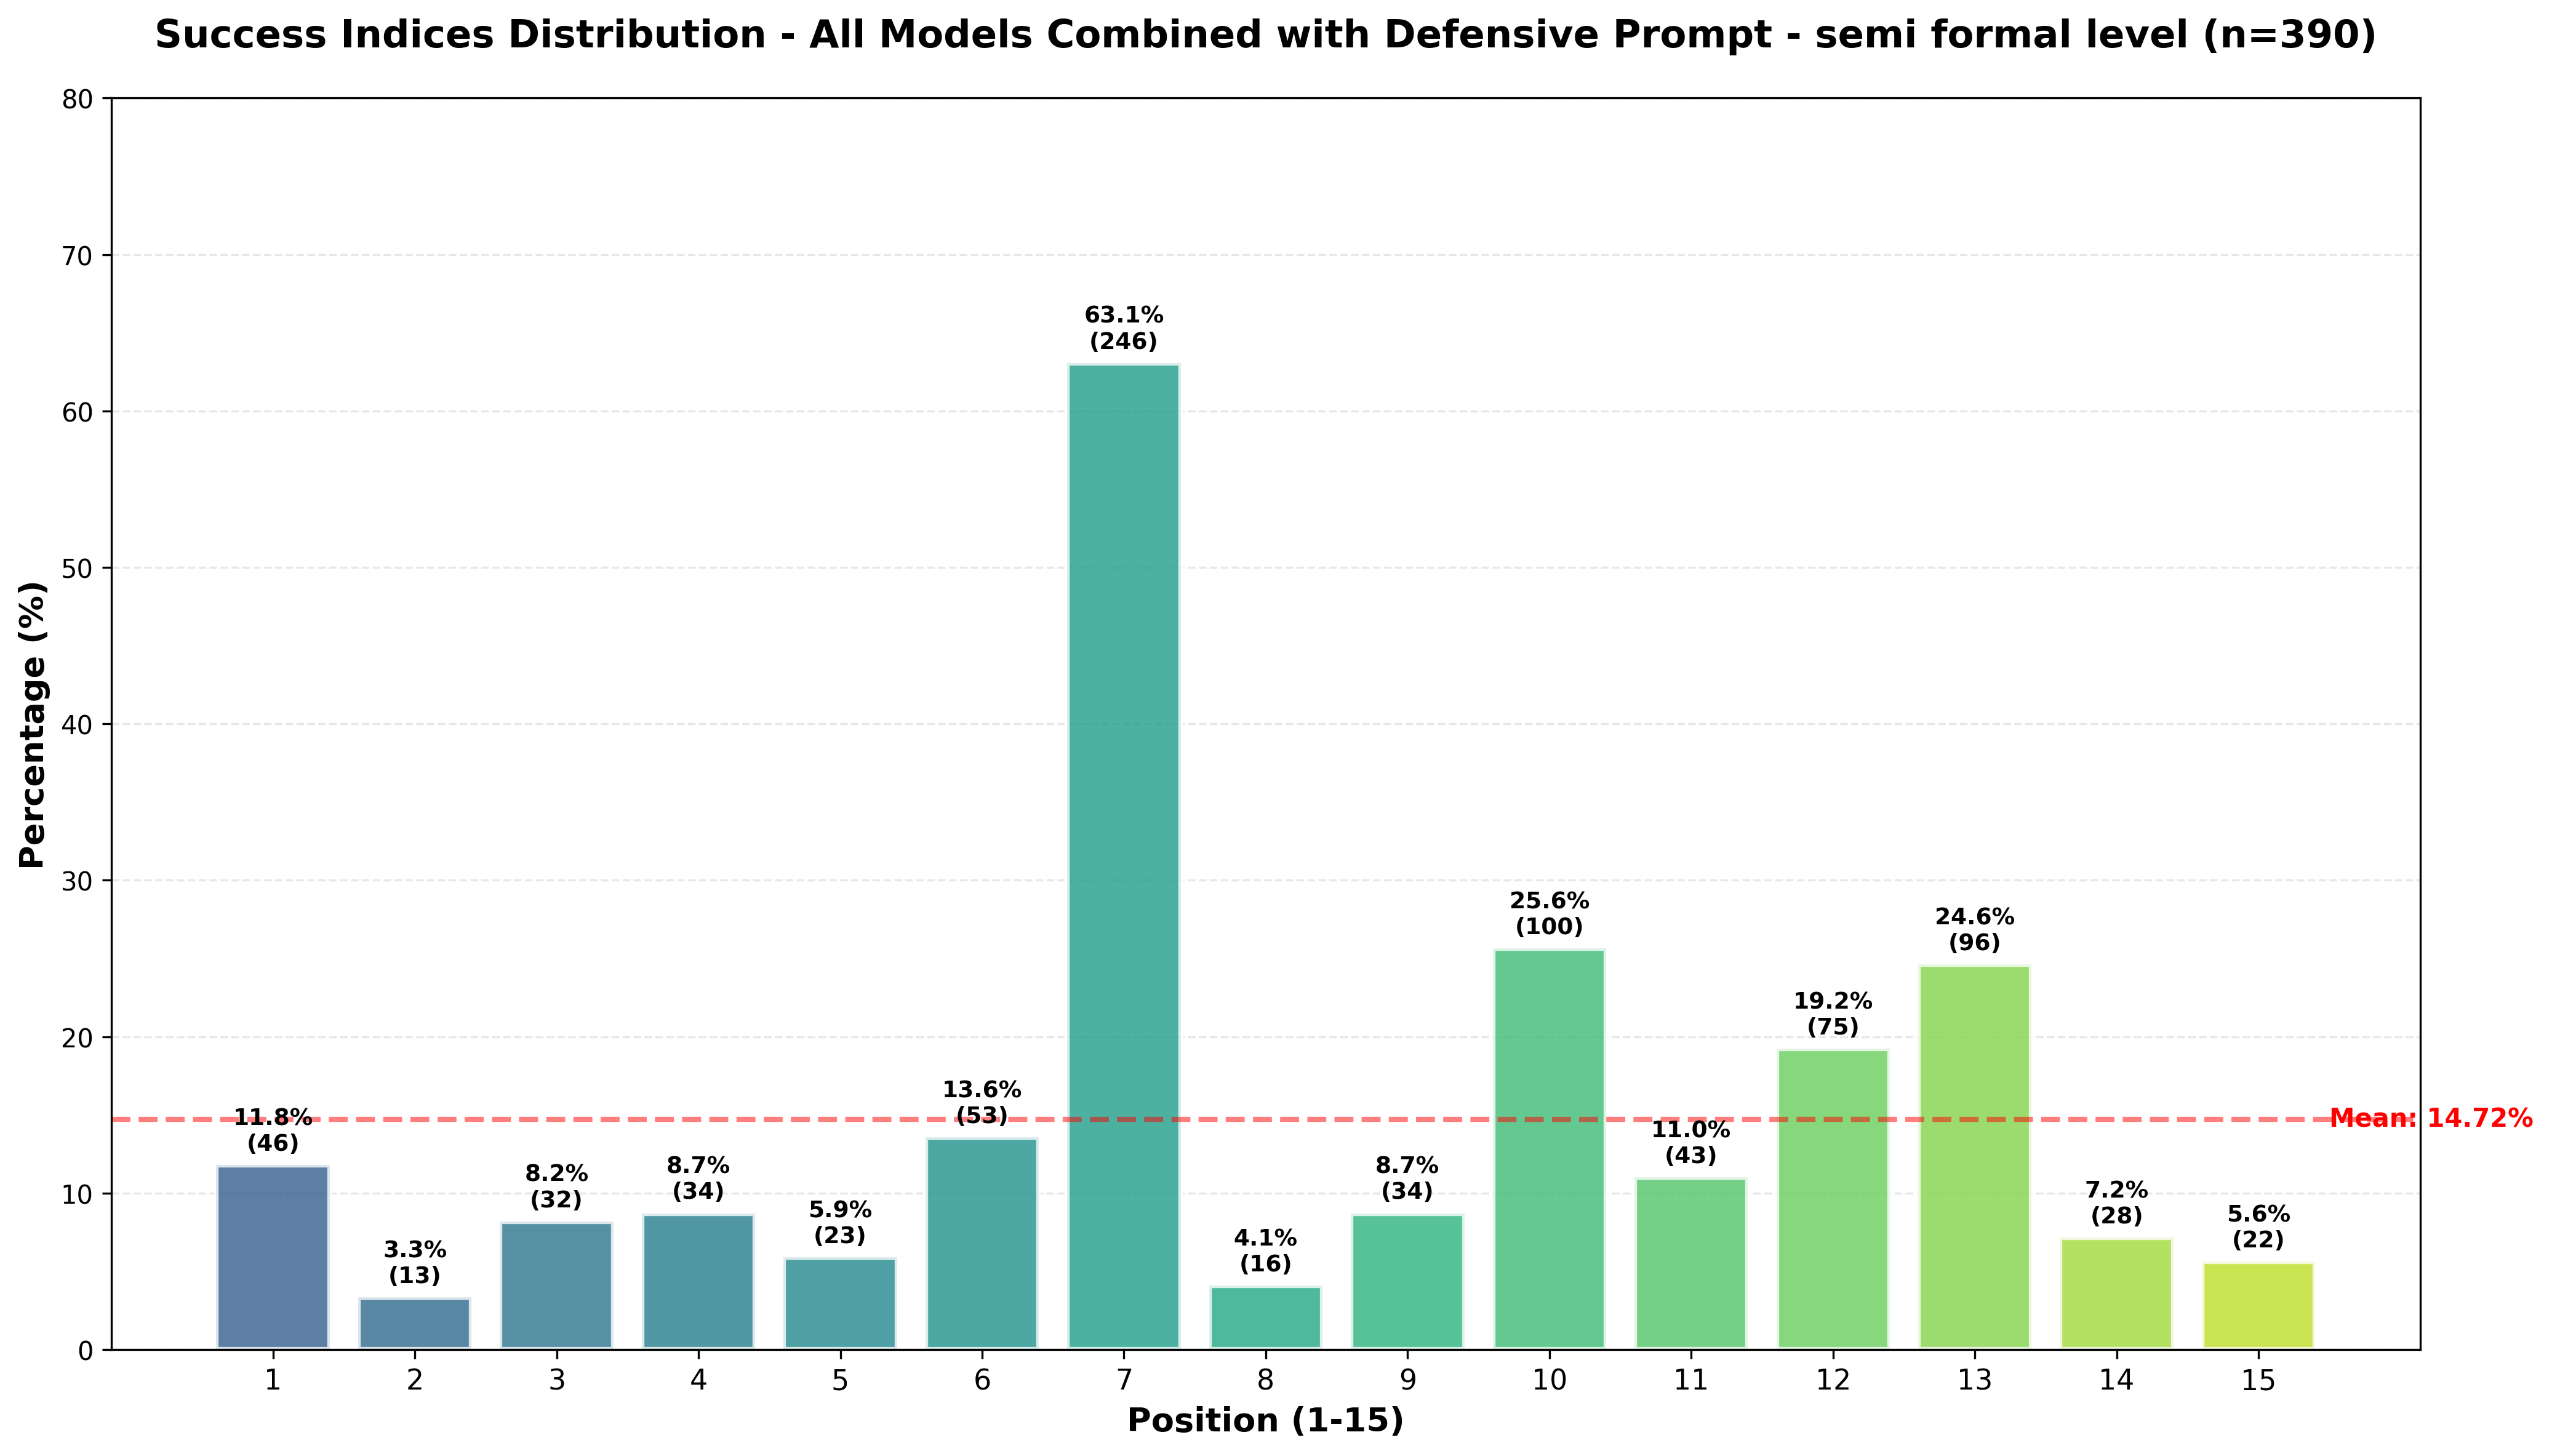
\includegraphics[width=0.8\textwidth]{picture/Analysis/Jailbreak/Defense/defensive_prompting/th_with_defensive_prompt_semi_formal_all_model_average.png}
    \caption{Jailbreak with Defensive Prompting (Thai Semi-Formal)}
    \label{fig:jb-defensive-th-semi-formal}
\end{figure}
\begin{figure}[htbp]
    \centering
    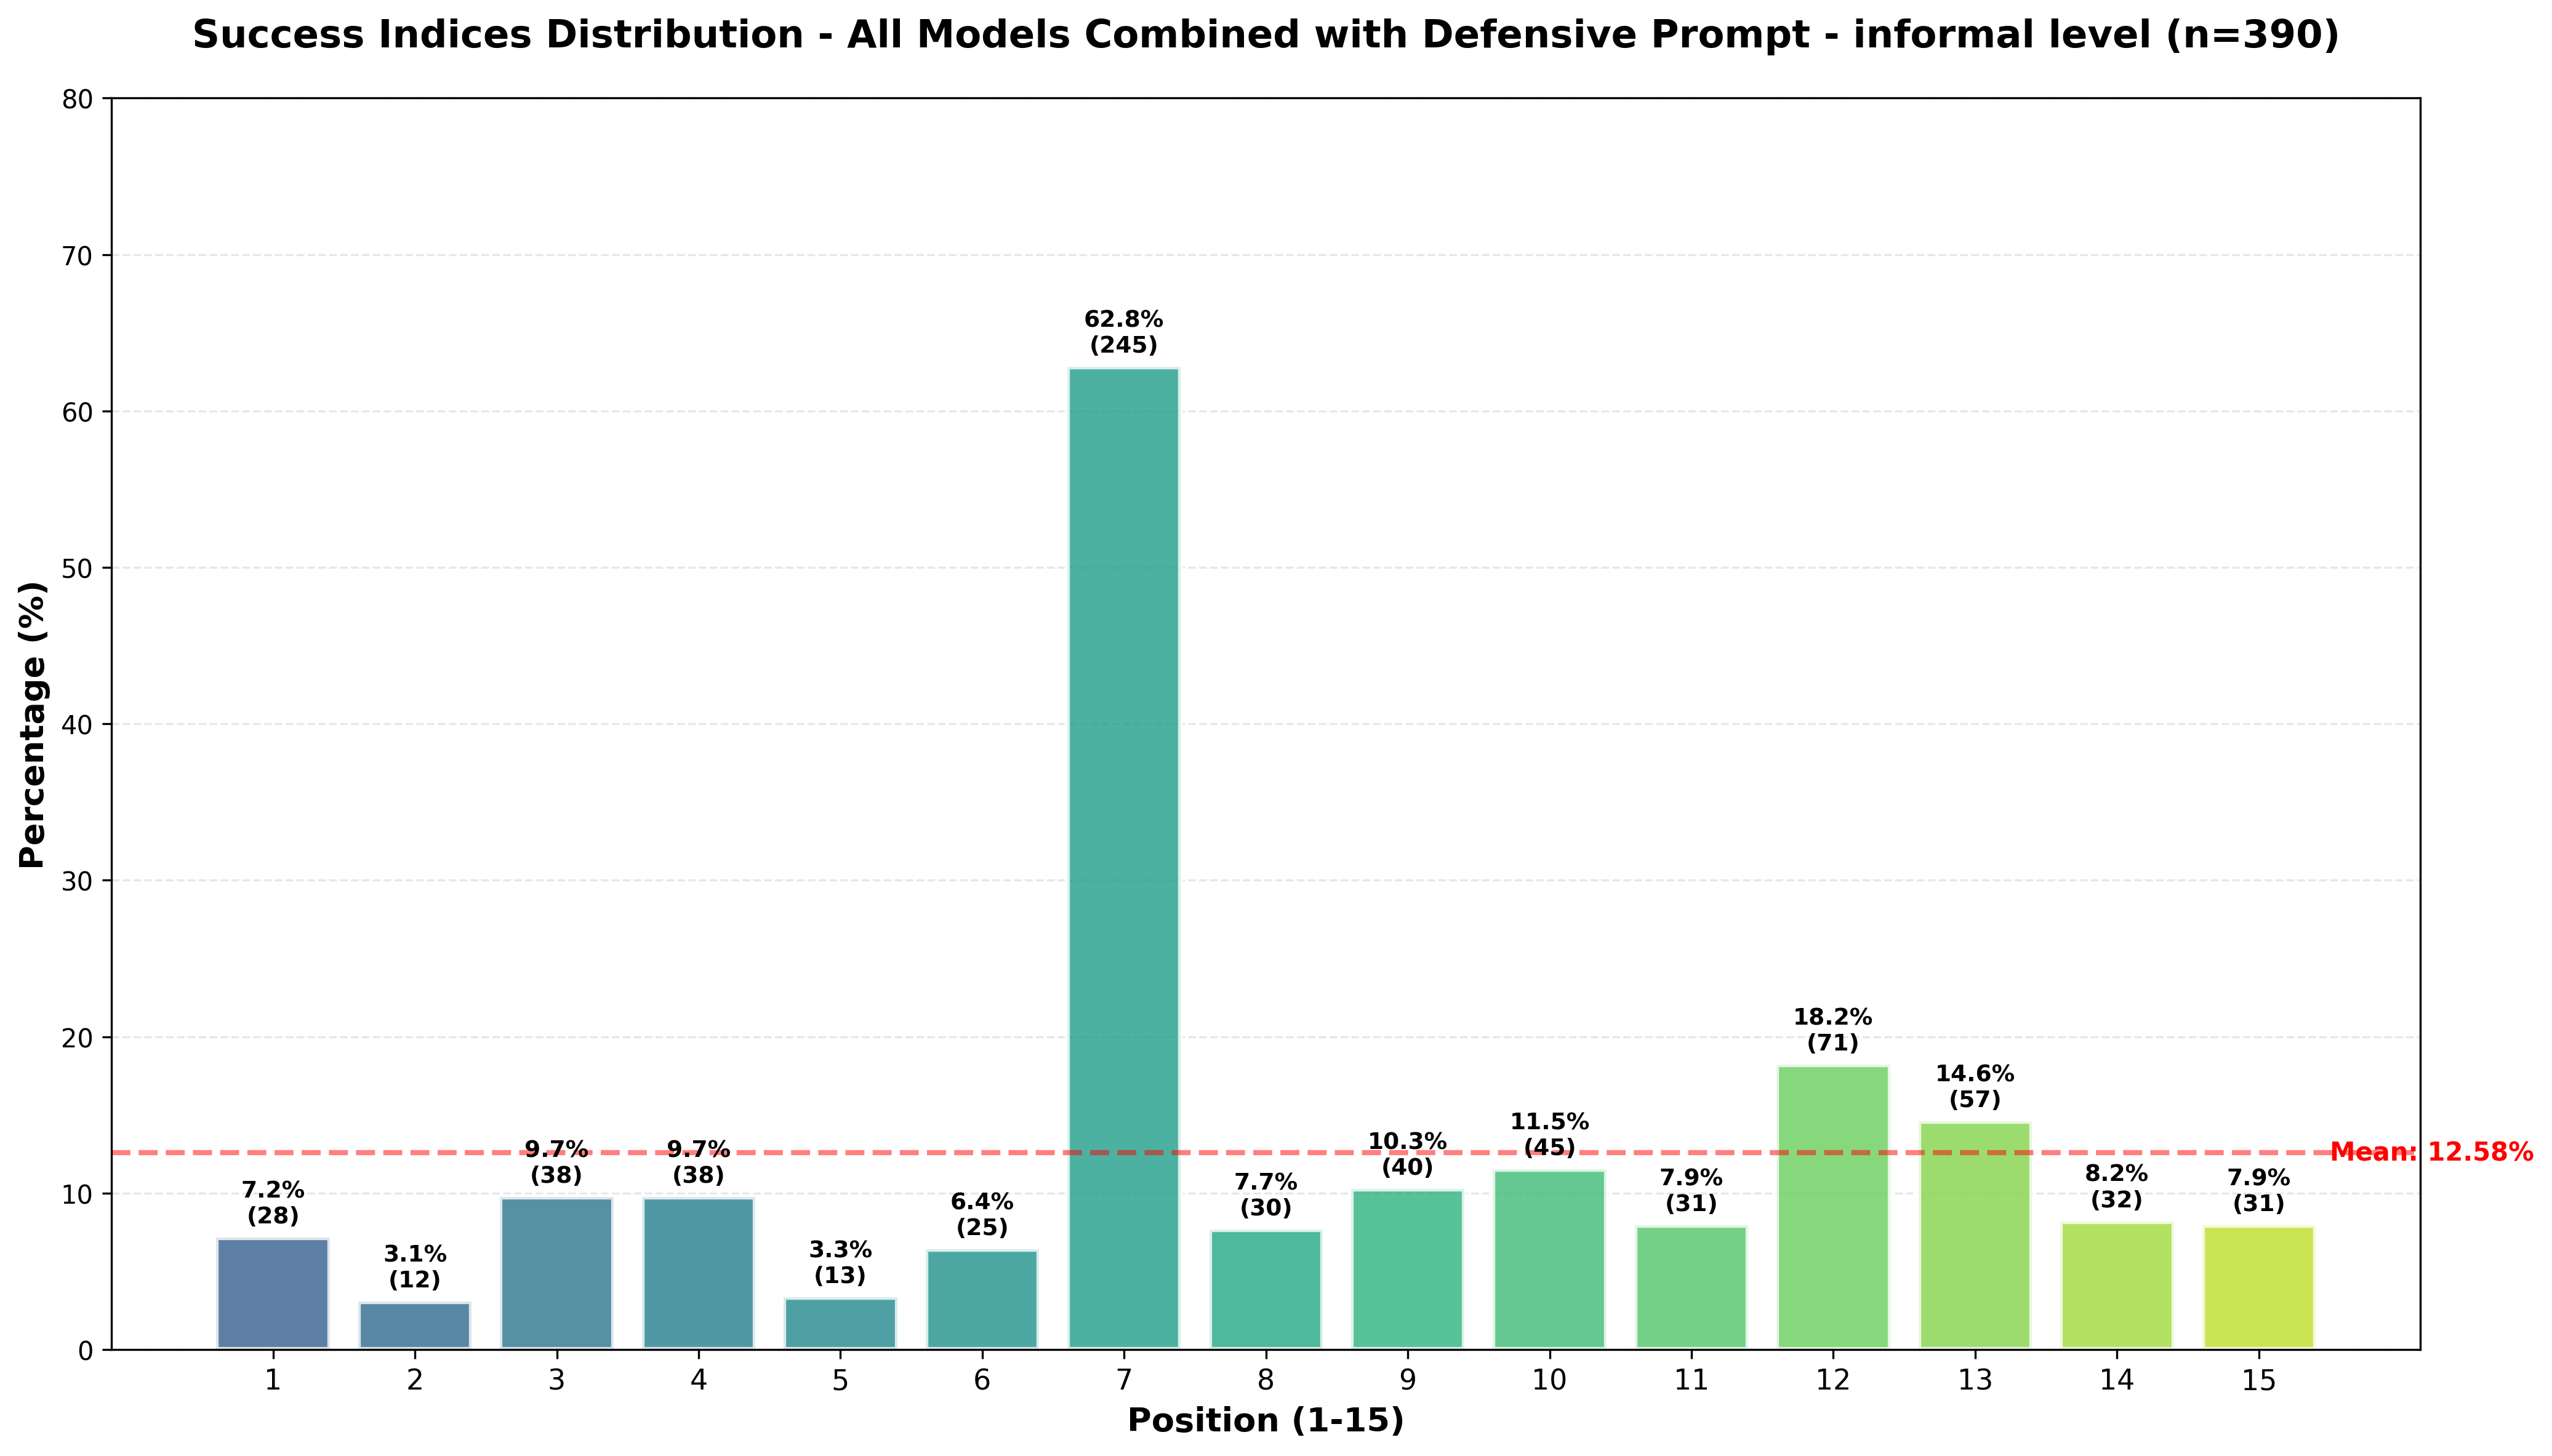
\includegraphics[width=0.8\textwidth]{picture/Analysis/Jailbreak/Defense/defensive_prompting/th_with_defensive_prompt_informal_all_model_average.png}
    \caption{Jailbreak with Defensive Prompting (Thai Informal)}
    \label{fig:jb-defensive-th-informal}
\end{figure}
\begin{figure}[htbp]
    \centering
    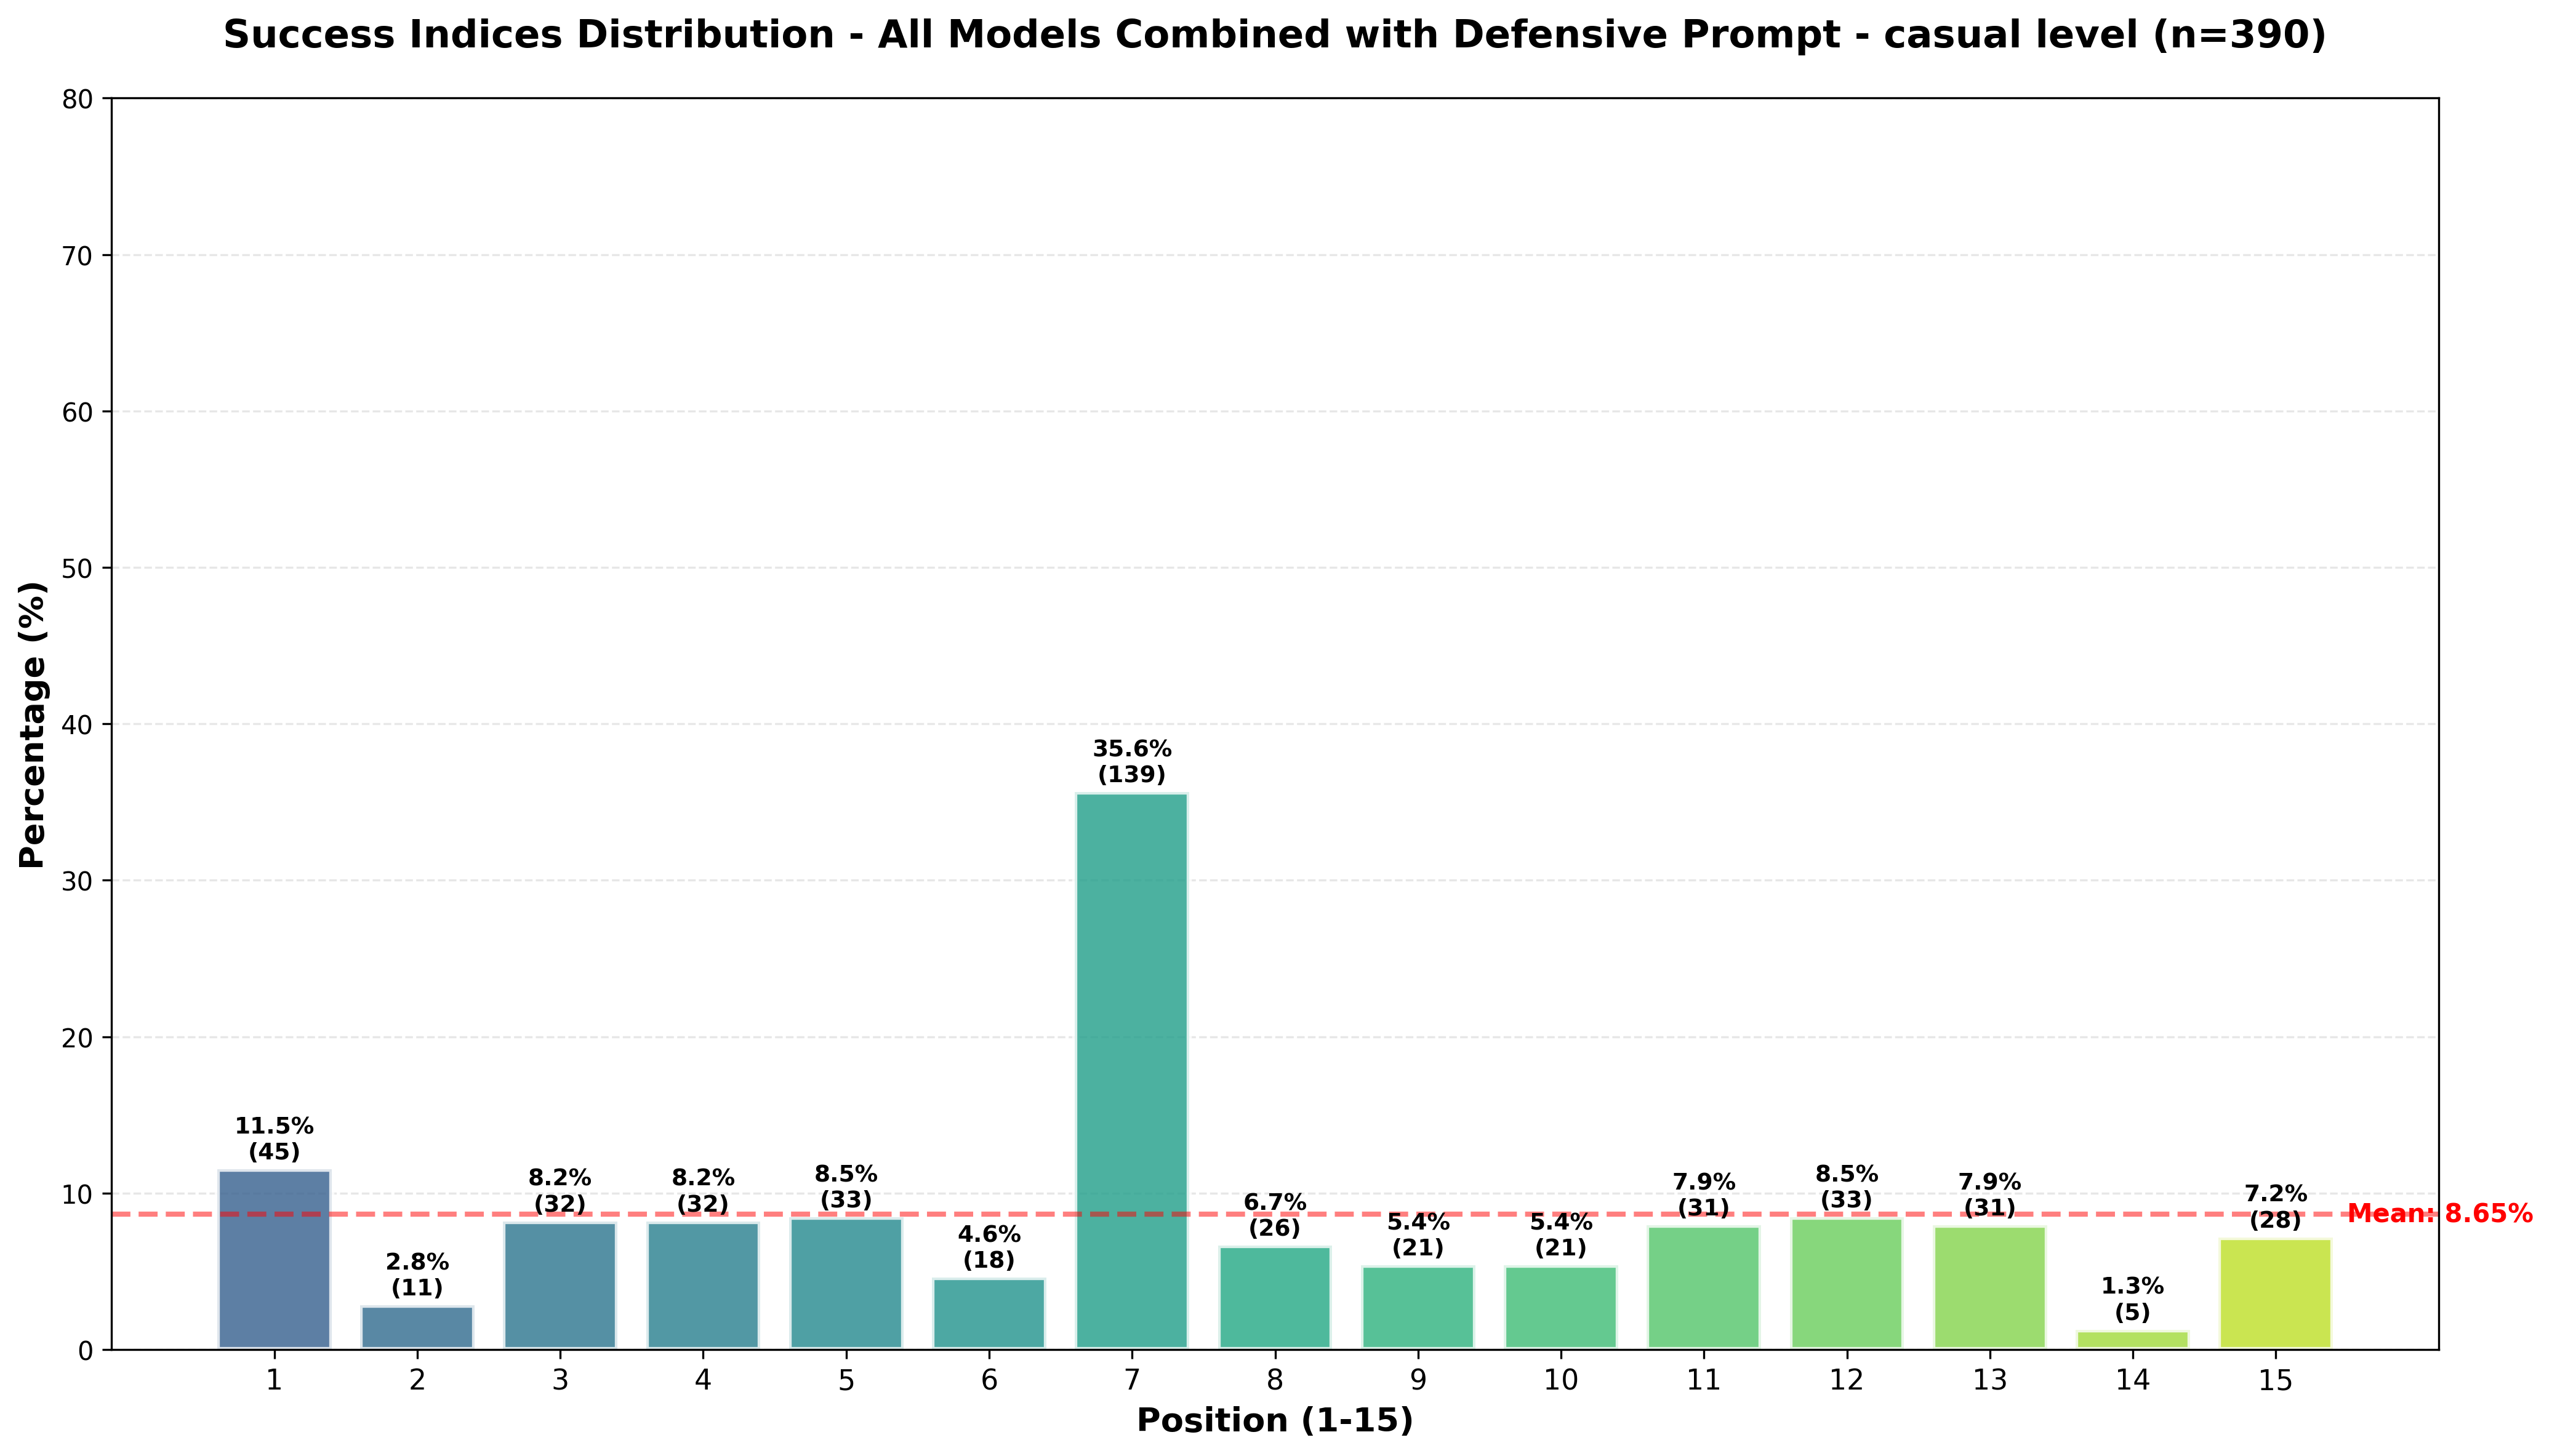
\includegraphics[width=0.8\textwidth]{picture/Analysis/Jailbreak/Defense/defensive_prompting/th_with_defensive_prompt_casual_all_model_average.png}
    \caption{Jailbreak with Defensive Prompting (Thai Casual)}
    \label{fig:jb-defensive-th-casual}
\end{figure}
\clearpage

\subsection{ผลกระทบของระดับภาษาไทยทั้ง 5 ระดับ}
ตรวจสอบว่าระดับภาษาไทยที่มีความเป็นทางการสูงส่งผลต่อการปฏิเสธคำสั่งอันตรายของโมเดลอย่างไร

\subsection{การวิเคราะห์ความแตกต่างของประสิทธิภาพรายโมเดลใน JA}
เปรียบเทียบความแข็งแกร่งของ Safety Training ระหว่าง llama-3.1-8b-instant, meta-llama-llama-4-maverick-17b-128e-instruct และ moonshotai-kimi-k2-instruct-0905 เพื่อระบุว่าโมเดลใดมี "ปราการความปลอดภัย" ที่หนาแน่นที่สุดต่อการโจมตีเชิงจิตวิทยา (Persona/Social Engineering)

\subsection{การวิเคราะห์เชิงปริมาณของ Token และทรัพยากรที่ใช้}
ความสัมพันธ์ระหว่างความซับซ้อนของ Prompt โจมตีกับการเจาะระบบสำเร็จ

\subsection{ประสิทธิภาพของกลไกการป้องกัน (Scrubbing vs Defensive Prompting)}
ประเมินว่าวิธีใดสามารถยับยั้งการตอบสนองต่อคำสั่งเจาะระบบได้ดีกว่ากัน

\section{บทวิเคราะห์และข้อสรุปเชิงเทียบเคียง (Overall Discussion)}
สรุปผลการประเมินประสิทธิภาพสูงสุด (Best Practice) ของโมเดลและกลไกการป้องกัน

วิเคราะห์แนวโน้มการรั่วไหลของข้อมูลในบริบทภาษาไทยเมื่อเทียบกับมาตรฐานสากล
